\documentclass[12pt]{report}
% Intended to be built with pdflatex.
% Labeling convention example: \label{ssec:acknowledge}.
%   Specifically, use (<=4)-letter class (e.g. chap, sec, ssec, fig, etc.),
%   followed by a colon, followed by a shortish underscore separated name
%   (e.g. intro, nu_energy_spectrum).

% packages
\usepackage{amssymb}              % for \gtrsim
\usepackage{amsmath}              % for \text, align, split ...
\usepackage{booktabs}             % for \toprule
\usepackage{graphicx}             % for \includegraphics
\usepackage{hyperref}             % for \url and \href
\usepackage{mbdeaton}             % include my special macros
\usepackage{natbib}               % allows me to define the citation style
\usepackage{setspace}             % for \doublespacing
\usepackage{subcaption}           % for subfigure
\usepackage{wsudissertation}      % definitions for WSU-specific formatting

% initializations
\doublespacing                    % use \begin{singlespace} ... \end{singlespace}
                                  % for stretches of monospace text
\bibliographystyle{abbrvnat}                 % set bibliography style
\setcitestyle{authoryear,open={(},close={)}} % set citation style not numeric

% *******************************************************************************
\begin{document}
\pagenumbering{roman}

% *******************************************************************************
\begin{titlepage}
  \begin{singlespace}
    \begin{center}
      {\uppercase{
          Neutrinos in Mergers of\\
          Neutron Stars with\\
          Black Holes}}\\
      \vspace{1.63in}
      By\\
      \bigskip
      \uppercase{Michael Brett Deaton}\\
      \vspace{2.65in}
      A dissertation submitted in partial fulfillment of\\
      the requirements for the degree of\\
      \bigskip
      \uppercase{Doctor of Philosophy}\\
      \bigskip \bigskip \bigskip
      \uppercase{Washington State University}\\
      Department of Physics and Astronomy\\
      \bigskip
      \uppercase{May 2015}\\
      \bigskip \bigskip
      $\copyright$ Copyright by MICHAEL BRETT DEATON, 2015\\
      All Rights Reserved
    \end{center}
  \end{singlespace}
\end{titlepage}
\newpage

% *******************************************************************************
\thispagestyle{empty} %\addtocounter{page}{-1}
\begin{center}
  \begin{singlespace}
    \null % necessary to get \vfill to work without initial text
    \vfill
    $\copyright$ Copyright by \uppercase{Michael Brett Deaton}, 2015\\
    All Rights Reserved
  \end{singlespace}
\end{center}
\newpage

% *******************************************************************************
\begin{singlespace}
  \noindent
  \vspace{1.5in}

  \noindent To the Faculty of Washington State University:\\
  
  The members of the Committee appointed to examine the dissertation of
  \uppercase{Michael Brett Deaton}
  find it satisfactory and recommend that it be accepted.
  
  \begin{flushright}
    \signhere{Matthew D.\ Duez, Ph.D., Chair}\\
    \signhere{Sukanta Bose, Ph.D.}\\
    \signhere{Guy Worthey, Ph.D.}
  \end{flushright}
\end{singlespace}
\newpage

% *******************************************************************************
\begin{center}
  \uppercase{Acknowledgements}
  \addcontentsline{toc}{section}{Acknowledgements} % insert into TOC
\end{center}

  \bigskip
  My advisor, Matt Duez, wrote the core of the general relativistic hydrodynamics
  code that I used to evolve the models in this work. I am grateful for his
  mentorship in research and teaching. His reasoning is always clear and
  enlivening. My colleague Francois Foucart is the co-author of that code.
  Without the robust simulation tool they developed, I could not have done this
  work. In addition, Matt, Francois and another colleague, Evan O'Connor, passed
  on their knowledge of hydrodynamics, thermodynamics, and radiation transport
  through discussions, emails, video conferences, and during my visit to the
  University of Toronto. My colleague, Andy Bohn, wrote the ray-tracing code our
  collaboration uses to find event horizons in arbitrary vacuum spacetimes. His
  clear coding style and generous correspondence made it easy for me to co-opt
  large parts of his work for my own ray-tracing code. Many other colleagues gave
  me a bit of their time and knowledge: particularly Jeff Kaplan, Mark Scheel,
  B\'ela Szil\'agyi, Curran Muhlberger, and Daniel Hemberger.
  Christian Ott and Francois thoroughly read and commented on each draft of
  \citealt{deat2013-leakage} (Chap.~\ref{chap:leakage} of this thesis), and
  my writing grew in stature and wisdom and in favor with God and man.

  My colleague and friend Fatemeh Hossein-Nouri helped in countless debugging
  sessions, shared her relativistic intuition, and introduced me to Hafiz.
  My friends Dan Helms, Ryan Niemeyer, Dusty Vaughn, Phillip Jacobs, and Riley
  Rex were the most excellent friends.
  My friend Joseph Halbert sent me a timely reminder to keep pumping my legs.
  My mom and dad, Mike and JoEtta, were early and late guides.
  One of my favorite undergraduate professors, Mike Sadler, crossed paths with me
  at every April APS Meeting. Once, after one of my talks,
  he told me directly and gently, ``I didn't understand how your findings could
  be tested,'' and I've taken that to heart.

  Finally, my wife and companion, Darci, has lit up the last half of my graduate
  studies with her own probing intellect and love. This work bears the imprint
  of some of her questions.

\newpage

% *******************************************************************************
\begin{center}
  \begin{singlespace}
    \addcontentsline{toc}{section}{Abstract} % insert into TOC
    \label{ssec:abstract}

    {\uppercase{
        Neutrinos in Mergers of\\
        Neutron Stars with\\
        Black Holes}}\\
    \bigskip
    Abstract\\
    \bigskip \bigskip \bigskip
    by Michael Brett Deaton, Ph.D.\\
    Washington State University\\
    May 2015\\
    \bigskip \bigskip \bigskip
    Chair: Matthew D.\ Duez
  \end{singlespace}
\end{center}
  
Mergers of a neutron star and a black hole are interesting because of the dual
complexity of strong gravity and nuclear-density fluid. In this dissertation,
I present a model of such a merger and its remnant accretion disk, useful in
teaching us about the role of neutrinos in these events.
\newpage

\tableofcontents
\newpage

\listoftables
\addcontentsline{toc}{section}{List of Tables} % insert into TOC
\newpage

\listoffigures
\addcontentsline{toc}{section}{List of Figures} % insert into TOC
\newpage

\begin{center}
  \null
  \vspace{2.7in}
  \bigskip
  To my dad, Mike Deaton.\\
  For love and curiosity.
  \newpage
\end{center}
\pagenumbering{arabic}

% Overview
\chapter{Overview}
\label{chap:overview}

Neutron stars and stellar-mass black holes form out of massive stars when they
exhaust their nuclear fuel. White dwarfs form in the same way, but from less
massive stars, with $M\lesssim 8\,M_{\odot}$, like our sun.
For stars of $M\gtrsim 8\,M_{\odot}$, generally the more massive
($M\gtrsim 20\,M_{\odot}$) end up as black holes, and the less massive
($M\lesssim 20\,M_{\odot}$) end up as neutron stars
\citep{woos2002-review_stellar_evolution}.

Unlike main-sequence stars, which are supported against gravitational collapse
by thermal pressure due to nuclear burning, neutron stars and white dwarfs
don't burn fuel; their composition is fixed.
Their resistance to collapse, in the language of quantum mechanics, is due
to degeneracy pressure, a physical manifestation of the uncertainty principle.
Neutron stars are supported by degenerate neutrons, while white dwarfs are
supported by degenerate electrons. In contrast to both of these, black holes
are the unique objects which, in equilibrium, are not supported against
collapse. They are so compact that gravity overwhelms all of Nature's repulsive
forces, and their surfaces fall inside a causal horizon. After this, gravity
enforces a one-way flow of matter and radiation inward.

Both neutron stars and white dwarfs are limited by a maximum mass above which
gravitational pressure overwhelms degeneracy pressure. Neutron stars with masses
greater than $\sym2\,M_\odot$, or white dwarfs with masses greater than
$\sym1.4\,M_\odot$, cannot exist in equilibrium: they are unstable against
collapse to a black hole.

Neutron stars and black holes are called compact objects because their enclosed
mass per surface radius, or compactness $\mathcal{C}\equiv G M/c^2 R$, is very
large:
$\mathcal{C}_{\rm BH}=0.5$ and
$\mathcal{C}_{\rm NS}\sim0.15$,
whereas $\mathcal{C}_{\rm WD}\sim10^{-4}$, and $\mathcal{C}_{\odot}\sim10^{-6}$.
\todo{check $\mathcal{C}_{\rm WD}$ and $\mathcal{C}_{\odot}$}
Because gravity plays a greater role at lesser distances from a massive object,
a body's compactness is a measure of the significance of gravity
in explaining changes to that body and its immediate environment.
For neutron stars and black holes, gravity is very important.

Binaries of compact objects may form by two evolutionary channels: from the
double supernovae of a pair of main sequence stars already in binary orbit,
or from dynamical capture in dense stellar regions, like globular clusters,
where near-flybys are common.
\todo{cite ... maybe Stephens+}
In either case, when two compact objects orbit each other closely, gravitational
theory predicts \citep{eins1916-integrate_field_eqns,eins1918-grav_waves}
and observations confirm \citep{will2014-review}
that their orbit slowly shrinks. Orbital energy and angular momentum
are transported away from the system by gravitational waves.

Compact binaries come in three combinations: black hole--black hole \bhbh,
neutron star--black hole \nsbh, and neutron star--neutron star \nsns.
At the writing of this thesis,
the only known compact binary systems are ten neutron star--neutron star
\nsns binaries \citep{post2014-evolution_compact_binaries}; no compact binaries
involving a black hole have yet been discovered.
Becuase all the known systems comprise neutron stars---which are radio-visible as
pulsars, blinking at exquisitely regular intervals---excellent orbital timing
information is available for them.

In fact, we can watch the gravitational drain of orbital energy in many
cases, the most famous being the Hulse-Taylor neutron star--neutron star \nsns
binary \citep{huls1975-discovery}.
Since radio astronomers began tracking it in 1974, its 7.75~hr orbit has
shortened by a few milliseconds \citep{weis2010-hulse_taylor_timing}.
% Estimate based on orbital params on 52984.0 MJD (12.11.03):
% \Delta P = P_b*\dot{P_b}*24*3600 [= 70 ns per orbit]
% N        = 365.24/P_b            [= 1130 orbits per yr at end 20th Cent]
% \Delta T = N*40*\Delta P         [= -3 ms per 40 yrs at end 20th Cent]
At this rate, the two neutron stars will touch in $\sym$300~million years,
% from simple integration:
% T_merge  = P_b/\Delta T          [= 300 Myrs]
at which time the quiescent binary will go through a number of violent changes.
This is called merger.

\section{Are Neutron Star--Black Hole Mergers Common?}
\label{sec:how_common}

Astrophysicists use the small collection of known neutron star--neutron star
binaries \nsns to predict the merger rate of such systems in the local universe.
From the ? known systems at the time of publication, Kalogera et al.\
\citeyearpar{kalo2004-bns_merger_rate, kalo2004-erratum} extrapolated ?
\todo{fill in}
mergers per Milky-Way-equivalent-galaxy per million years.
Neither black hole--black hole \bhbh nor neutron star--black hole \nsbh
merger rates can be extrapolated from observations.

However, at least one possible progenitor to a neutron star--black hole \nsbh
binary is known: Cygnus X-1. Cygnus X-1 (discovered by ?)
\todo{citealt Bowyer+ 1965}
is an x-ray source whose energetic and rapidly-flickering emission
is well-modeled as a $\sym15\,M_\odot$ black hole orbiting a $\sym20\,M_\odot$
main-sequence companion.
\todo{cite Wong+ 2012}
Several evolution scenarios are possible, with a small probability of forming
a compact binary that could merge.
\citet{belc2011-cyg_x1}
explore these scenarios, and from their relative likelihoods, draw conclusions
about the rate of neutron star--black hole \nsbh mergers in our galaxy.
In ? million years,
\todo{check}
the companion star will exhaust its nuclear fuel and its core will collapse,
triggering a supernova. It may form a neutron star, which, if the asymmetry of
the explosion isn't so great as to gravitationally unbind it from the black hole,
will yield a neutron star--black hole \nsbh binary. In less than 1\% of the possible
scenarios, the compact binary forms close enough to merge within the age of the
Universe. If the only formation channel is through
binaries like the one that formed the Cygnus X-1 system, there must be very few
neutron star--black hole \nsbh binaries in our galaxy, and the merger rate observable
by Advanced LIGO is 1 detection every 30-250~years.
\todo{check}
\todo{introduce LIGO}

%\subsubsection{Theoretical Answers}
%\label{sssc:theory}
Theoretical astrophysicists have pursued a more comprehensive approach to this
calculation through population synthesis studies: the modeling of large numbers
of stars representative of populations observed in our own and nearby galaxies.
The models attempt to capture the particular nuclear effects, gravitational
interactions, stellar evolutions, and supernova dynamics of millions of binaries,
to reach an ultimate conclusion about the compact remnants in each system:
binary or no? and if yes, is the binary orbiting closely enough to merge in
$10^{10}$~yrs, the age of our Universe?
Population synthesis models are attended by large uncertainties
(see especially \citealt{domi2012-merger_rates_part1}).
But one attempt to bracket these uncertainties
has revealed that at the current age of the Universe,
field populations of neutron star--black hole \nsbh binaries are probably
merging at a rate between $\ll1$ and $\sym10$
per year per Gpc$^3$, with the most likely rates near 1~yr$^{-1}$~Gpc$^{-3}$
\citep[Figs.~3 and~5]{domi2013-merger_rates_part2}.
According to this study, and with good agreement between a range of models,
the local neutron star--black hole merger rate peaked long ago,
around $z\sim3$, as high as $50\text{--}100$~yr$^{-1}$~Gpc$^{-3}$.
\todo{compared to \nsns, much more common in low-z galaxies}
This range of rates gives us a theoretical answer to the question,
``how common are neutron star--black hole mergers?''.

%\subsubsection{Observational Answers}
%\label{sssc:observation}
These theoretical predictions may be complemented or challenged by observations.
In the next few years, astronomers expect to record the final seconds to minutes
\todo{check}
of the gravitational wave signal emitted by a compact binary
as it merges, using gravitational wave interferometers like LIGO, Virgo, and Geo.
\todo{cite AdvLIGO white paper}
Or if matter is at hand, that is, if one or both of the objects is a neutron
star, they may observe electromagnetic or neutrino signals. Let's discuss
electromagnetic signals here; in Sec.~\ref{ssec:neutrino_roles}, we will
turn to neutrinos.

A diverse family of electromagnetic signals is possible from a neutron
star--neutron star \nsns or neutron star--black hole merger \nsbh:
\begin{itemize}
  \item Kilonova: Some of the neutron star material may be ejected and escape
    from the system. As this neutron-rich matter expands and cools, exotic heavy
    nuclei form like ice crystals in a winter pond. These nuclei only form in a
    low-energy bath of free neutrons via rapid neutron capture, the r-process.
    Days later, these unstable nuclei decay and, like a nuclear power reactor,
    heat the ejecta, causing it to emit photons with a
    thermal spectrum, at optical or infrared frequencies.
    \citep{
      li1998-transients,
      robe2011-transients,
      metz2012-most_promising,
      kase2013-opacities}.

    Recently space-based infrared telescopes observed a short glow that
    fit these theoretical predictions
    \citep{berg2013-130603B,tanv2013-130603B}. This excited the astronomical
    community because it was days after and at the same sky position as a gamma
    ray burst, described below.
  \item Late radio afterglow: The distant neighborhood of the merger, the
    circumburst medium, is often denser than the binary's immediate environment.
    \todo{often?}
    The circumburst medium may be simply the interstellar medium.
    \todo{what else?}
    If any mildly-relativistic unbound material (e.g.\ neutrino- or
    electromagnetic-driven winds) interacts with this denser medium, it
    experiences hydrodynamic shocks, amplifying any seed magnetic fields, and
    causing the plasma to emit radio-frequency synchrotron radiation.
    This signal could persist for weeks after the merger
    \citep{naka2011-radio}.

    No observations of such a signal have been found, but this is not surprising
    because of the weakness of the signal, which may be detectable out to
    $z\sim0.1$ \citep{naka2011-radio}.
  \item X-rays emission: If the progenitor is a neutron star--neutron
    star binary \nsns, the immediate product of the merger may be
    a supramassive neutron star,
    \todo{cite}
    more massive than the fundamental
    limit discussed above ($M\lesssim2\,M_\odot$), but nevertheless quasi-stable
    because it is rotating rapidly.
    If so, the supramassive neutron star may emit winds that shock
    into each other and emit thermal x-ray radiation \citep{rezz2015-two_winds}.
    Afterglows have been detected \citep{fong2012-xray_afterglow}, and in fact,
    so have x-ray precursors \citep{troj2010-sgrb_precursors}, which are
    not well-understood. One possible source for an x-ray precursor from either
    neutron star--neutron star \nsns or neutron star--black hole \nsbh mergers is
    the shattering of the neutron star's crust due to tidal forces
    \citep{tsan2012-shattering}.
  \item Gamma ray burst: If an accretion disk forms---either after the
    spin-down of the supramassive neutron star, or because a black hole forms
    immediately after merger, or because the progenitor is a neutron star--black
    hole \nsbh binary---some combination of magnetic and neutrino heating
    could drive an ultrarelativistic jet. The jet, when it shocks into the
    circumburst medium, or shocks internally, will emit high energy gamma ray
    photons, highly beamed in the direction of the jet, due to its relativistic
    motion \citep{eich1989-grb_bns,nara1992-grbs_nsns_bhns}.
    The burst of gamma ray emission lasts as long as the accretion is
    active enough to drive the jet, about a second.

    Many gamma ray bursts have been observed, following the first reports by
    \citet{kleb1973-first_report_grb}, and they fall roughly into two categories,
    long and short, with durations falling to either side of $\sym2$~s.
    The observed short gamma ray bursts have
    properties that are well-modeled by this merger--disk--jet scenario.
    One strong connection between these observations and the model proposed here
    is that short gamma ray bursts predominantly originate from galaxies with
    old stellar populations, precisely the galaxies in which we expect the most
    compact binaries.
\end{itemize}
Some of these electromagnetic signals are strong---in particular gamma ray
bursts---and our observing horizon is well past a gigaparsec.\footnote{
According to \citet{naka2007-review_sgrb} the population of short gamma ray
bursts with redshift measurements exhibit a median $z\approx0.25$, corresponding
to a comoving distance of $\sym1$~Gpc.}
During BATSE's operation (a NASA gamma-ray telescope aboard the CGRO satellite,
in orbit from 1991--2000), it detected a short gamma ray burst about once every
four days \citep{naka2007-review_sgrb}.
In an indirect sense, this rate gives us an observational answer to the question,
``how common are neutron star--black hole mergers?''.

But in the next few years a much more direct answer will be possible, as the
advanced generation gravitational wave interferometers, Advanced LIGO and Virgo,
begin to record and search gravitational strain data for the signature chirps of
compact binary mergers. Unless astrophysicsists are fundamentally
mistaken about the formation of compact binaries, the three-detector network of
Advanced LIGO's two instruments plus Advanced Virgo, when operating at design
sensitivity, will likely detect neutron star--black hole \nsbh mergers at a
rate of 0.1--10~yr$^{-1}$
\citep[Tables~2 and~3]{domi2014-merger_rates_part3}.\footnote{
I report here the most significant figure of the brackets given by their range
of models, assuming only inspiral waveforms are used in matched filter searches,
and that the network signal-to-noise ratio is set to a threshold of 10.
Their predictions for neutron star--neutron star \nsns
and black hole--black hole \bhbh merger detections are
2--7~yr$^{-1}$ and 4--2000~yr$^{-1}$.}
\footnote{
These results are unpublished at the writing of this thesis.
However, traditionally, estimates of merger rates have been reported from the
\citet{abad2010-rates} review, which drew heavily on less-sophisticated versions
of the population synthesis models used by \citet{domi2014-merger_rates_part3}.}

Of course it is possible the astrophysics community is mistaken.
The physical processes linking compact binary mergers to these
signals are not fully understood, an ignorance that partly motivates this thesis.
In fact, until astronomers observe one of these electromagnetic signals in
coincidence with a gravitational wave signal, it's possible (though very hard
for this physicist to imagine) that the short
gamma ray burst rate---providing the observational answer to our question
above---has nothing to do with mergers of compact binaries of any kind.

Though much in the next sections is applicable to any type of merger involving
a neutron star, let us focus in on neutron star--black hole \nsbh
mergers, the topic of this thesis. Sec.~\ref{sec:why_this_model} defends this
focus more extensively than here.
But briefly: in this study, we are interested in systems involving the
strongest gravitational effects and nuclear matter. The first interest leads us
to black holes, and the second interest leads us to neutron stars.
We won't pursue neutron star--neutron star
\nsns or black hole--black hole \bhbh binaries past this section.

\section{What Roles May Neutrinos Play?}
\label{sec:neutrino_roles}
Some neutron star--black hole mergers produce stellar mass accretion disks.
As matter in the disk flows from large distances to the
inner edge of the disk, where it plunges into the black hole, it loses
gravitational energy and gains kinetic and thermal energy, which escapes
as radiation. This energy transfer is immense. The velocity of gas in circular
Kepplerian orbit around mass $M_{\rm BH}$ at radius $r$
(easy to remember by the 1-2-3 rule: $GM_{\rm BH}^1=\Omega^2r^3$) is
\begin{equation}
  v = \Omega r  = (GM_{\rm BH}/r)^{1/2}, \nonumber
\end{equation}
where $G$ is Newton's gravitational constant.
Its specific energy is therefore
\begin{align}
  e &= \frac{1}{2}v^2-\frac{GM_{\rm BH}}{r} \nonumber \\
  &= -\frac{GM_{\rm BH}}{2r}. \nonumber
\end{align}
Because the gas velocity varies with $r$, the disk shears against itself. If the
fluid is viscous (which is likely, due to turbulence, magnetic fields, or even
radiative stresses),
\todo{cite each of these}
the fast inner regions slow down, and the slow outer regions speed up. The net
effect is that gas in the inner disk moves a little closer to the black hole,
increasing its specific energy:
\begin{equation}
  \Delta e = \frac{GM_{\rm BH}}{2}
  \left(\frac{1}{r_{\rm final}}-\frac{1}{r_{\rm initial}}\right). \nonumber
\end{equation}
This process transports gas inward until it plunges into the black hole.
If most of the disk accretes, the total increase in the energy of the gas
is $E_{\rm acc}\sim M_{\rm disk} \Delta e$. How much is that?

We may estimate $r_{\rm initial}$ by the radius of the disk. Simulations give
\todo{cite}
characteristic scales of:
\begin{align}
  R_{\rm disk} &\sim 100\,{\rm km} \nonumber \\
  M_{\rm disk} &\sim 0.01\text{--}0.5\,M_\odot. \nonumber
\end{align}
And we may estimate the inner edge of the disk by
\begin{eqnarray}
  r_{\rm final} &\sim& 1\text{--}9 \times \frac{GM_{\rm BH}}{c^2} \nonumber \\
  &\sim& 1.5\text{--}13.5 \,{\rm km}\times \left(\frac{M_{\rm BH}}{M_\odot}\right), \nonumber
\end{eqnarray}
the radius of last stable circular orbit around the black hole. The range of this
radius represents its dependence on the black hole's spin: the higher the spin
in the direction of the disk's rotation, the closer may the gas approach before it
plunges into the black hole.
Thus the gravitational energy released by a stellar-mass accretion disk is
\begin{equation}
  E_{\rm acc} \sim 10^{51\text{--}54} \,{\rm erg}. \nonumber
\end{equation}
This energy is initially transferred into the bulk motion of the gas, as it
spirals in toward the black hole. But turbulence and viscosity transfer it to
smaller scales: ordered kinetic energy becomes disordered thermal energy.
The disk heats up and radiates this energy at a supernova-scale luminosity:
\begin{equation}
  \label{eqn:L_order_mag}
  L \sim \frac{E_{\rm acc}}{100\,{\rm ms}}
  \sim 10^{52\text{--}55}
  \,{\rm erg \, s}^{-1},
\end{equation}
where we have used an accretion timescale of 100~ms, as determined by simulations.
\todo{cite}
Surprisingly, unlike most hot objects in the universe, the enormous energy output
of an accretion disk is not carried away by photons.
\todo{mention significance of compactness in this analysis}

\subsubsection{Radiative Energy Transport}
\label{sssc:nu_E_transport}
Photons scatter off of free ions and over a characteristic length of
$\lambda_\gamma\sim(2Y_e n_b\sigma_{\rm T})^{-1}$, where $2Y_e$ is the local
number ratio of ions to baryons, $n_b$ is the baryon number density, and
$\sigma_{\rm T}=6.6\times10^{-25}\,{\rm cm}^2$ is the cross section
for photons scattering elastically off of electrons. The disk being
neutron-rich, $Y_e$ is in the range of 0.1. And typical densities are a
few orders of magnitude less than the central density of a neutron star,
or $\rho\sim10^{11}\,{\rm g\,cm}^{-3}$,
so that $n_b=\rho/m_U\approx10^{-4}\,{\rm fm}^{-3}$.
A disk's photon optical depth (that is, the square root of the number of times
a photon scatters before it leaves the disk) is of order
\begin{align}
  \tau_\gamma &\sim \frac{R_{\rm disk}}{\lambda_\gamma} \nonumber \\
  &\approx (10^7\,{\rm cm})(0.1)(10^{35}\,{\rm cm}^{-3})(10^{-24}\,{\rm cm}^2)
  \approx 10^{17}, \nonumber
\end{align}
(where we have disregarded factors close to 1)
and the timescale for a photon to escape is
$T_{\gamma,\rm esc}\sim\tau_\gamma^2\lambda_\gamma/c\approx1$~million years, or
ten trillion times longer than the lifetime of the disk.
Photons can't carry away the thermal energy of the disk: they're trapped in it.

But neutrinos can. Neutrinos are freely produced in the neutron-rich matter.
The dominant weak interactions contributing to their scattering
are proportional (times a numerical factor close to 1)
\todo{too simplistic}
to the weak scattering cross section:
\begin{equation}
  \sigma_0
  \equiv \frac{4}{\pi}\left(\frac{\hbar}{m_e c}\right)^{-4}
  \left(\frac{G_F}{m_e c^2}\right)^2
  \approx 1.8 \times 10^{-44} \,\, {\rm cm}^2, \nonumber
\end{equation}
and scale with neutrino energy like $(\varepsilon_\nu/m_e c^2)^2$
\citep{tubb1975-neutrino_opacities,shap1983-bh_wd_ns}.
Neutrinos scatter primarily off of the free nucleons in the disk, so their
characteristic scattering length is $\lambda_\nu\sim(n_b\sigma_0)^{-1}$,
where $Y_e$ is the local number ratio of electrons to baryons.
A disk's typical neutrino optical depth is therefore
\begin{align}
  \tau_\nu
  &\sim \tau_\gamma \frac{\sigma_0}{\sigma_T} \left(\frac{\varepsilon_\nu}{m_e c^2}\right)^2 \nonumber \\
  &\approx 0.01\times\left(\frac{\varepsilon_\nu}{\rm MeV}\right)^2. \nonumber
\end{align}
In the post-merger accretion disk, fluid temperatures are $\sym10$~MeV (which
gives us the name `nuclear' accretion disk, since temperatures are comparable to
nuclear binding energies), and $\tau_\nu\sim1$.
Neutrinos are neither totally trapped nor totally free: they play a
significant role in energy transport in the disk.
In fact, simulations of nuclear accretion disks, with realistic neutrino
treatments (see Sec.~\ref{sec:history} and Chap.~\ref{chap:leakage}) yield neutrino
luminosities comparable to the power estimate from Eqn.~\ref{eqn:L_order_mag},
indicating that neutrinos serve to drain the gravitational energy released by
accretion.

\subsubsection{Composition Changes}
\label{sssc:composition}
But neutrinos don't just transport energy in and away from the accretion disk.
Because they carry lepton charge, neutrino absorptions change fluid composition
via the charged-current reactions:
\begin{align}
  \label{eqn:beta_n_to_p}
  \nu_e \, n \rightarrow e^{-} \, p       & \qquad {\rm increasing}\,Y_e, \\
  \label{eqn:beta_p_to_n}
  \bar{\nu}_e \, p \rightarrow e^{+} \, n & \qquad {\rm decreasing}\,Y_e.
\end{align}
where $\nu_e$ and $\bar{\nu}_e$ are electron-type neutrino and antineutrino,
$e^{-}$ and $e^{+}$ are electron and positron, and $n$ and $p$
are neutron and proton, respectively.
And neutrino emission, via the reverse reactions, also changes composition.
As $Y_e$ changes, the thermodynamic properties of the fluid change.
\todo{add discussion of first law}

If the fluid is hot, both neutrino and antineutrino luminosities are high,
and near the emission surface, they will annihilate at high enough efficiencies
(via $\nu\,\bar{\nu}\rightarrow e^{-}\,e^{+}$) to create a lepton pair plasma.
Neutrino annihilation heating is one process by which accretion may
power an ultrarelativistic jet, forming a gamma ray burst, as described in
Sec.~\ref{ssec:how_common}, and explored in our model in
Sec.~\ref{sec:q_this_case}.
\todo{cite early Piran paper}

\subsubsection{Neutrino Oscillations}
\label{sssc:neutrino_osc}
Also, when neutrino number densities are high,
\todo{necessary in vacuum oscillations?}
neutrinos can interact in a more subtle way: converting from one flavor into
another, by a process called neutrino oscillation.
(The Standard Model of particle physics predicts three neutrino flavors,
corresponding to the three generations of leptons: electrons, muons, and tauons.
\todo{`generations'?}
Each neutrino has a corresponding antineutrino, yielding six distinct neutrino
species: $\nu_e$, $\bar{\nu}_e$, $\nu_\mu$, $\bar{\nu}_\mu$, $\nu_\tau$,
and $\bar{\nu}_\tau$.)
\todo{mass$\neq$flavor eigenstates}
Neutrino flavor oscillations were first proposed in 197?
\todo{find/cite}
and were later found to explain the long-standing solar physics problem in which
neutrino observatories measured an otherwise unexplainable deart of $\nu_?$-type
\todo{which $\nu$?}
neutrinos from the Sun. Further theoretical explorations in the context of
supernovae have revealed that
\todo{cite}
the presence of matter can significantly amplify the oscillation likelihood.
Another amplification of the electron-type oscillation can arise if the
$\bar{\nu}_e$ self-interaction potential is greater than the $\nu_e$ potential.
\todo{cite Malkus+2014}
(The self-interaction potential at any given point in space is a function of
neutrino energies, number densities, and the angular spread of incoming
neutrinos.) All of these conditions may obtain in and around a post-merger
nuclear accretion disk. Collective oscillations would change the neutrino
signal detected from a nearby merger, and could suppress or amplify neutrino
interactions with nearby matter, for example the nucleosynthesis processes
described below.

\subsubsection{Nucleosynthesis}
\label{sssc:nucleosynthesis}
The eventual fate of matter in a neutron star--black hole merger is to drain
across the one-way boundary of the horizon. From then on, its only effect on
the universe outside the black hole is a gravitational effect.
However, in some mergers, depending on the intrinsic sizes and spins of the
two bodies, and on the eccentricity of their final orbits, some fraction of the
neutron star matter may be ejected and escape, as mentioned in
Sec.~\ref{sec:how_common} \citep{latt1974-bhns_ejecta}.
Matter may become gravitationally unbound from the central bodies by dynamical
ejection or by radiation pressure, or by plasma interactions with magnetic
fields.
Such matter, originally free baryons and leptons, will go through a change of
composition as it leaves the merger environment, expanding and cooling.
Heavier nuclei will form from its free nucleon and light-nuclei constituents.
This process, called nucleosynthesis, can be dramatically modified by neutrino
irradiation, both heating up the escaping fluid, and changing its composition.
For example, with simplifying assumptions for their accretion disk model,
Surman et al.\ 2014
\todo{fix cite}
showed in one case, that $\nu_e$ radiation dominated over $\bar{\nu}_e$
unexpectedly, causing large amounts of $^{}56$Ni to form, instead of the
heavier lanthanides expected when $\bar{\nu}_e$ dominates.

\subsubsection{Direct Detection}
\label{sssc:nu_detection}
Finally, neutrinos emitted during merger and accretion could be detected by
existing and future neutrino observatories. Neutrinos, as we showed earlier,
carry away most of the thermal energy generated in a neutron star--neutron star
\nsns or neutron star--black hole \nsbh merger, because photons are trapped in
the dense matter. And neutrinos are produced copiously in nuclear matter at
temperatures above $\sym1$~MeV.
\todo{check/cite}
Neutrino luminosities are of the order $10^{53}\,{\rm erg\,s}^{-1}$. Even
though neutrinos interact very weakly with matter, detectors are in operation
that could detect a neutrino signal this strong from a merger in the
Milky Way Galaxy.
\todo{cite Caballero/McGlaughlin 2009}.

\section{How Long Does it Take?}
\label{sec:timescales}
The main timescale of a neutron star--black hole merger is the dynamical
timescale. This is the time over which gravity causes changes to the fluid.
As we will see, it is essentially unchanging throughout the merger.
This is an astonishing fact, since at the beginning, the fluid is essentially
static in the neutron star, and at the end it is highly dynamical, in the disk.
The dynamical timescales associated with these two fluid configurations are:
\begin{align}
  T_{\rm dyn,star} &\approx (G\rho)^{-1/2} \nonumber \\
  T_{\rm dyn,disk} &\approx 2\pi/\Omega. \nonumber
\end{align}
where $G$ is Newton's gravitational constant, $\rho$ the star's density,
and $\Omega$ the angular frequency of the disk.
Before merger, the neutron star's central density is
$\rho\sim10^{14}\,{\rm g\,cm}^{-3}$---thus $T_{\rm dyn,star}\approx0.5$~ms.
After merger, the bulk of the disk orbits the black hole at a distance of
a few horizon radii, where the Kepplerian orbital angular frequency for a black
hole of a few solar masses is
$\Omega\sim1000\,{\rm rad\,s^{-1}}$---thus $T_{\rm dyn,disk}\approx0.5$~ms.

(As an aside, we can see the correspondence between these two dynamical
timescales by using Keppler's law, $GM=\Omega^2 R^3$, from
Sec.~\ref{sec:neutrino_roles},
to write $\Omega^{-1}=(R^3/GM)^{1/2}=(G\rho)^{-1/2}$.
In this sense, the fact that $T_{\rm dyn}$ doesn't change over the different
epochs of the merger is not so surprising, since the fundamental gravitational
scales of the problem, mass and length, are basically of order $1\,M_\odot$
and $10$~km throughout.)

So the main timescale of a neutron star--black hole merger is of order
$T\sim1$~ms.
For a physical description of the changes occuring in a complex system---like
the one at hand, involving gravity, electromagnetism, nuclear interactions, and
radiation---timescales guide us in making powerful simplifications.
If a particular subset of physics has a timescale
$T_{\rm slow\, process}\gg T$, we can ignore it:
its related physical quantities may be fixed at their initial level.
If some other subset of physics has a timescale
$T_{\rm fast\, process}\ll T$, we can also ignore it:
its related physical quantities may be averaged over a cycle (if the process
is periodic) or set at some quasi-equilibrium value (if the process is secular).

\subsubsection{Gravitational Radiation}
The gravitational radiation timescale is how long it takes for gravitational
waves to change the system. We may also think of it as the time till merger.
The relativistic dynamics of the merger
are nonlinear, and when the binary is in close orbit, this timescale can only
be computed numerically. However, at large separations, when the bodies are
moving much slower than the speed of light, $v/c\ll1$, a linear approximation
\todo{PN? what order?}
can be made (see for example, \citealt[Sec.~16.4]{shap1983-bh_wd_ns}):
\begin{equation}
  T_{\rm grav} \approx \frac{5}{256}\frac{c^5}{G^3}\frac{R^4}{M^2\mu},
\end{equation}
where $M=m_1+m_2$, and $\mu \equiv m_1 m_2/(m_1+m_2)$, and $a$ is the semi-major
axis of the orbit, $R$ for extreme mass ratio binaries, and $2R$ for equal mass
binaries.
\todo{is that right?}
Even when the binary is in close orbit, this approximation is correct to order
of magnitude.
\todo{calculate for our system}

Gravitational radiation is, therefore, an important process to consider in the
merger.

\subsubsection{Particle Interactions}
Strong nuclear forces act on a timescale of $10^{-21}\,{\rm s}$ at the high
\todo{check/cite}
densities of the neutron star, and the high temperatures and densities of the
merger. This is the timescale over which
nuclei form and dissociate. It is so small compared to the main timescale of
of the merger, that we may consider the nuclear reactions to be in equilibrium.
This is the nuclear statistical equilibrium assumption, by which the fluid's
composition of relative particle species may be entirely parameterized by a
single parameter, the electron fraction $Y_e$.

But the weak force is much...weaker.
The weak timescale, or how long it takes $Y_e$ to change due to the charged
current reactions (Eqns.~\ref{eqn:beta_n_to_p} and~\ref{eqn:beta_p_to_n} and
their reverse processes) is
\begin{equation}
  T_{\rm weak} \approx \frac{M}{m_U} \frac{\langle Y_e \rangle}{R_\nu},
\end{equation}
where $M$ is the total fluid mass, $m_U$ the average nucleonic mass,
$\langle Y_e \rangle$ the average electron fraction, and
$R_\nu \equiv R_{\nu_e}-R_{\bar{\nu}_e}$ the net lepton number carried
away by neutrinos.
Simulations, like the one presented in this thesis (see
Fig.~\ref{fig:neutrinos_by_species}, have shown that
$R_\nu\gtrsim10^{57}\,{\rm s}^{-1}$.
For a fraction of a solar mass of material, $M/m_U\sim10^{56}$~baryons.
The electron fraction of a neutron star is very low, and we may estimate
$\langle Y_e \rangle\sim0.1$. Thus $T_{\rm weak}\sim10$~ms. Of course, to
compute this estimate, we assume the disk changes homogeneously; in fact,
some regions radiate neutrinos more luminously than others, and the weak
timescale in more luminous regions is much shorter.
Weak processes, then, are important to consider in the merger.

%\subsubsection{Radiation}
%The radiation timescale is the time over which the radiation field responds
%to changes in the matter. If the matter is transparent, that is the neutrino
%mean free path $\lambda_\nu$ is larger than the length scale of fluid variations
%$L$, neutrinos emitted from one side travel to the other side in
%a light-crossing time,
%\begin{equation}
%  T_{\rm rad,\, free} \approx \frac{L}{c}.
%\end{equation}
%If, however, the matter is opaque, that is the neutrino mean free path is
%smaller than fluid length scales, neutrinos emitted from deep within the fluid
%experience many scatterings before escaping to the outer reaches. The radiation
%field changes on a diffusion timescale,
%\begin{equation}
%  T_{\rm rad,\,diff} \approx \frac{\lambda_\nu}{c}.
%\end{equation}

\section{What's the History Behind this Study?}
\label{sec:history}
As we found in the previous sections, neutrinos are interesting and important
players in neutron star--black hole mergers.
What has the astrophysics community already learned about them
in this context?\footnote{
some of this section is reproduced from \citealt[Sec.~1]{deat2013-leakage}}

Because the accretion disk spans neutrino-opaque and neutrino-transparent regimes
(see Sec.~\ref{sec:neutrino_roles}), a full six-dimensional evolution of the
neutrino fields (1 energetic + 3 spatial + 2 angular dimensions) is needed
to completely describe the coupling between radiation and matter.
This is impossible with current computational resources. Fortunately, many of
the essential features of the radiation can be captured using a simple
leakage scheme. Rather than performing actual radiation transport, leakage
schemes remove energy and alter lepton number at rates based on the local
free-emission and diffusion rates. Leakage certainly neglects some arguably
important effects (for example, neutrino-driven winds), but it captures
the basic energetics and composition drift of the post-merger system.
For an analysis of the limitations of this approximation in the context of
core-collapse supernova simulations, see \citet{ott2013-cc_leakage}.
\todo{indicate following review is mostly about leakage}

Neutrino leakage simulations have been used to build models of neutron
star--neutron star \nsns mergers since the late 1990s
\citep{
ruff1996-leakage_part1,
ross2002-leakage_part1}.
\citet{jank1999-leakage_bhns} and \citet{ross2004-leakage_bhns} developed models
of neutron star--black hole \nsbh mergers using Newtonian gravity, with
phenomenological treatments of relativistic effects like the back reaction of
gravitational waves on the fluid, and the orbital instability at radii close to
the black hole.
These models predict neutrino luminosities of $10^{51\text{--}53}\rm\,erg\,s^{-1}$.

Leakage techniques have recently been incorporated into general relativistic
simulations of stellar core collapse
\citep{seki2011-cc_leakage, ott2013-cc_leakage}
and neutron star--neutron star \nsns mergers
\citep{seki2011-nsns_leakage,kiuc2012-nsns_leakage_hyperons}.
But the first relativistic neutron star--black hole simulations with a
nuclear treatment of the fluid and neutrino feedback were presented in
\cite{deat2013-leakage}, reproduced in Chap.~\ref{chap:leakage}.

\section{Why this Particular Model?}
\label{sec:why_this_model}
In this thesis, I focus our attention on neutron star--black hole mergers, and in
particular, on one model of such a merger, with a specific set of initial
parameters. In this section, I explain that narrow focus.

Neutron star--neutron star \nsns and neutron star--black hole \nsbh mergers are
similar in many respects. They both evolve through an epoch dominated by
gravitational wave emission: inspiral, during which their orbits rapidly decay.
In both types of mergers, the neutron stars experience strong tidal forces,
distorting them into oblate spheres, and finally disrupting them.
And except for very low mass neutron star--neutron star \nsns binaries, with
total masses not exceeding the maximum neutron star mass, $\sym2\,M_\odot$,
all instances of both types of merger end up finally in the same state, a
single black hole with no matter nearby.

But the epoch between neutron star disruption and final black hole quiescence
may be quite distinct between these two classes of mergers. Generally, neutron
star--neutron star \nsns mergers yield a rapidly spinning blob of more than
$2\,M_\odot$ of matter, a supramassive neutron star,
supported against collapse, briefly, by centrifugal effects.
On the other hand, neutron star--black hole \nsbh mergers transition directly
to the disk stage, or else the neutron star is swallowed whole immediately upon
disrupting, and no disk forms.

In this work I focus on neutron star--black hole mergers \nsbh, where the
accretion epoch plays a central role. Furthermore, though both classes of
merger can disperse nuclear matter into the interstellar medium via winds and
dynamical ejection, the latter effect can be much more significant
in neutron star--black hole
mergers because of the greater compactness of the black hole, and therefore
stronger tidal forces experienced by the neutron star.
In this and future work, I am especially
interested in this dynamical ejecta, its role in galactic nucleosynthesis,
and its potential to emit a detectable flash of light. Also, though by most
predictions neutron star--black hole mergers are the least likely compact
binary merger to be detected by gravitational wave interferometers
(see Sec.~\ref{sec:how_common}),
they are detectable at a greater distance than are neutron star--neutron star
\nsns mergers. This is because the
strength of the peak gravitational wave signal scales with the total mass,
and the average stellar mass black hole is likely many times as massive as the
average neutron star ($10\,M_\odot$ vs.\ $2\,M_\odot$; see, for example,
up-to-date tables of observed compact object masses
at \url{http://stellarcollapse.org}).

In this work I present one model of a neutron star--black hole merger,
with a high black hole dimensionless spin of
$a^* \equiv J_{\rm BH}c/GM_{\rm BH}^2 =0.9$ aligned with the binary's orbital
angular momentum,
component masses of $M_{\rm BH}=5.6\,M_\odot$ and
$M_{\rm NS}=1.4\,M_\odot$,
and a neutron star radius of 12.7~km,
so that the mass ratio is $q \equiv M_{\rm BH}/M_{\rm NS}=4$,
and the neutron star compactness is
$\mathcal{C}_{\rm NS} \equiv G M_{\rm NS}/R_{\rm NS}c^2=0.16$.
We are particularly interested in these binary parameters because such a system
yields a massive accretion disk.

Heuristically it makes sense that $a*$, $q$, $M_{\rm BH}$, and
$\mathcal{C}_{\rm NS}$ have an effect on the amount of matter remaining outside
the black hole after tidal forces cause the neutron star to disrupt.
Tidal forces behave approximately as $M_{\rm BH} R_{\rm NS}/r^3$,
which can be evaluated at the radius of the last stable circular orbit,
inside of which the neutron star plunges, 
\begin{equation}
  \label{eqn:tidal_forces}
  F_{\rm tidal} \propto
  \left(q \,\mathcal{C}_{\rm NS}\, M_{\rm BH} \,f(a^*)^3\right)^{-1},
\end{equation}
where $f(a^*) \equiv M_{\rm BH}/r_{\rm ISCO}(a^*)$ decreases monotonically with increasing
prograde spin, and $r_{\rm ISCO}$ is the radius of the last (a.k.a\ inner-most)
stable circular orbit. Even this simple relationship indicates that
tidal disruption forces at the last stable circular orbit are greater for smaller
$q$, smaller $C_{\rm NS}$, smaller $M_{\rm BH}$, and larger $a^*$.
Simulations across the parameter space confirm these trends
\citep{pann2010-disk_mass,fouc2012-disk_mass}.

In fact, these four parameters are not independent. Since the compactness of a
cold neutron star is completely specified by its mass\footnote{we are
assuming the equation of state of neutron star matter is known}, we can write
Eqn.~\ref{eqn:tidal_forces} as
\begin{equation}
  F_{\rm tidal} \propto
  \left(q^2 \,\mathcal{C}_{\rm NS}(M_{\rm NS})\, M_{\rm NS}\, f(a^*)^3\right)^{-1},
\end{equation}
which describes a three-dimensional parameter space of possible mergers:
$\{q,M_{\rm NS},a^*\}$.
Furthermore, these parameters are constrained by observed populations. We
choose to study $M_{\rm NS}=1.4\,M_{\odot}$, a canonical neutron star mass, near
the center of the observed masses.\footnote{see
\url{http://stellarcollapse.org/nsmasses}}
This choice fixes the compactness of the star, and leaves $q$ and $a^*$
independently specifiable.
Field populations of black holes are observed to lie roughly in the mass range
5--20~$M_\odot$\footnote{see \url{http://stellarcollapse.org/bhmasses}},
but the spin range is poorly constrained.
\todo{find obs spin review}
To maximize disk mass we choose a black hole mass toward the bottom of this
range, $M_{\rm BH}=5.6\,M_\odot$, and a black hole spin toward the top of this
range, $a^*=0.9$.
\todo{use foucart model to predict $M_{\rm disk}$}

\section{What's the Scope and Trajectory of this Thesis?}
\label{sec:scope}

At the heart of this thesis, I present a model of a neutron star--black hole merger,
accounting in an approximate way for the major effects of neutrinos on the
post-merger accretion disk (Chap.~\ref{chap:leakage}).
This model then provides a starting point from which to examine the properties of
the radiation, in particular the spatial, energy, and angular distribution of the
escaping neutrinos
(Chap.~\ref{chap:ray_tracing}, Secs.~\ref{sec:f_algorithm}--\ref{sec:f_this_case}).
Finally, I use the neutrino distributions inferred from the model to investigate
the energetics of a very important astrophysical process: the formation of a
neutrino-driven jet which could power a short gamma ray burst
(Chap.~\ref{chap:ray_tracing}, Secs.~\ref{sec:q_algorithm}--\ref{sec:q_this_case}).

In addition to a reference section on conventions (Sec.~\ref{sec:conventions}),
Chap.~\ref{chap:intro} provides a technical introduction to the two physical
frameworks for the model presented here:
fluid dynamics (Sec.~\ref{sec:gr_hydro}) and
radiation transport (Sec.~\ref{sec:rad_transport})
in strong gravity.

I have aimed the preceding chapter in a general direction, toward students from
other fields than physics; the remainder is aimed squarely at physicists.


% Introduction
\chapter{Technical Introduction}
\label{chap:intro}

% Notation Conventions
% Brett Deaton -- Spring 2015

\section{Conventions}
\label{sec:conventions}

I adopt the standard general relativists metric signature convention
$(-,+,+,+)$.
In Chap.~\ref{chap:leakage}, I use natural geometric units
in which Newton's gravitational constant $G$, and the speed of light $c$, have unit
value; In the other chapters, I make $G$ and $c$ explicit.

I use abstract tensor notation in general: a tensor typeset with its indeces
represents the geometric object in all of its coordinate freedom. In other words
$T^{\alpha \beta}$ is identical to $T$, and is not $T$'s $\alpha\beta$-th
component.
In some equations, I use coordinate index notation accompanied with a warning.
Spatial tensors are given indices from the Latin alphabet ($a,b...$);
they exist on a 3-dimensional manifold. Spacetime tensors are given indices from
the Greek alphabet ($\alpha,\beta...$); they exist on a 4-dimensional manifold.
In instances of coordinate index notation, it follows naturally that
$\alpha,\beta...\in\{1,2,3\}$ and $a,b...\in\{0,1,2,3\}$.

Of course some symbols have labels other than their tensor indeces.
In particular, I use subscript labels before tensor indeces (e.g.\ the
momentum of a neutrino is $p_{\nu \alpha}$). I allow context to clarify when
an index ranges over some set other than dimension (e.g.\ the momentum of the
i-th flavor of neutrino is $p_{\nu_i \alpha}$). The subscript $\nu$ is always
used as a label, not as a tensor index.

\begin{table}
  \centering
  \begin{tabular}{rll}
    \textbf{Symbol}       & \textbf{Object}           & \\%\textbf{Additional Notes} \\
    $n_b$                 & baryon number density     & \\
    $\rho$                & rest density              & $\rho \equiv m_U n_b $ \\
    $\epsilon$            & specific internal energy  & not including the mass energy \\
    $h$                   & specific enthalpy         & $h=1+\epsilon+P/\rho$\\
    $P$                   & pressure                  & \\
    $T$                   & temperature               & \\
    $T^{\alpha \beta}$    & stress-energy tensor      & \\
    $Y_e$                 & electron fraction         & $Y_e=n_e/n_b$\\
    $\rho_*$              & density evolution variable& $\rho_*=\sqrt{g}W\rho$ \\
    $\tilde\tau$          & energy evolution variable & $\tilde\tau=\rho_*(hW-1)-\sqrt{g}P$ \\
    $\tilde S$            & momentum evolution variable & $\tilde S=\rho_*hu_i$\\
    $v^i$                 & Lagrangian velocity       & a.k.a.\ transport velocity, $v^i=u^i/u^t$ \\
    $u^\alpha$            & fluid four-velocity       & $u^a=dx^a/d\tau$ \\
    $U^\alpha$            & observer four-velocity    & used if we want to distinguish from $u^\alpha$ \\
    $d\tau$               & spacetime interval        & $d\tau=-dx^a dx^b \psi_{ab}$ \\
    $W$                   & Lorentz factor            & $\alpha u^t$ (if no gravity $W=1/\sqrt{1-v^2}$) \\
    $\tau$                & optical depth             & \\
    $Q_\nu$               & local energy emission rate& \\
    $R_\nu$               & local lepton number rate  & \\
    $\mu$                 & chemical potential        & $\mu=T\eta$ \\
    $p_\alpha$            & momentum 1-form           & \\
    $\varepsilon$         & neutrino energy           & used for asymptotic and local \\
    $\psi_{\alpha\beta}$  & spacetime metric          & \\
    $g_{ij}$              & spatial metric            & \\
    $\beta^i$             & shift                     & where $\beta_i = \beta^j g_{ij}$ \\
    $\alpha$              & lapse                     & \\
  \end{tabular}
  \caption[Symbols used in the text]{
    Some symbols used in this text.
    Indices are used in the ``Symbol'' column in an abstract sense, and in the
    ``Additional Notes'' column in a component sense.
  }
  \label{tab:conventions}
\end{table}

\begin{table}
  \centering
  \begin{tabular}{rlll}
    \textbf{Symbol} & \textbf{Value}       & \textbf{Units}           & \textbf{Description} \\
    $G$             & $6.67\times10^{-8}$  & cm$^3$ g$^{-1}$ s$^{-2}$ & Newton's gravitational constant \\
    $c$             & $3.00\times10^{10}$  & cm s$^{-1}$              & speed of light in vacuum \\
    $k_{\rm B}$     & $8.62\times10^{-11}$ & MeV K$^{-1}$             & Boltzmann's constant \\
    $G_{\rm F}$     & $2.3\times10^{-22}$  & cm MeV$^{-1}$            & Fermi coupling constant \\
    $G_{\rm F}/(\hbar c)^3$ & $1.17\times10^{-11}$ & MeV$^{-2}$       & ", naturalized units, $\hbar=c=1$ \\
    $\sin^2\theta_w$& 0.231                &                          & weak-mixing angle \\
    $m_e$           & 0.511                & MeV c$^{-2}$             & mass of electron \\
    $m_U$           & 939                  & MeV c$^{-2}$             & average nucleon mass, $(m_n+m_p)/2$ \\
    $M_\odot$       & $2.00\times10^{33}$  & g                        & solar mass \\
    $\hbar$         & $6.58\times10^{-22}$ & MeV s                    & reduced Planck's constant, $h/2\pi$ \\
  \end{tabular}
  \caption[Physical constants used in the text]{
    Some physical constants used in this text. Taken from the Particle Data
    Group, Particle Physics Booklet \citep{oliv2014-pdg}.
    I am only interested in scales, so I use three significant figures here.
    Note, the conversion factor between $G_{\rm F}$ in cgs and
    naturalized units is the naturalized length scale,
    $\hbar c/\varepsilon=1.97\times10^{-11}/(\varepsilon/{\rm MeV})$~cm.
  }
  \label{tab:constants}
\end{table}


\section{General Relativistic Hydrodynamics}
\label{sec:gr_hydro}
Here we introduce the equations describing the transport of particle number,
momentum, and energy by massive particles in the continuum limit, that is
\todo{specify ``continuum limit''}
a fluid.

Fluid dynamics are described in curved spacetime by the general relativistic
hydrodynamics equations:
\begin{align}
  \label{eqn:hydro_mass}
  \nabla_\alpha \rho u^\alpha &= 0 \\
  \label{eqn:hydro_mom}
  \nabla_\alpha T^{\alpha\beta} &= 0,
\end{align}
where $\nabla_\alpha$ is the covariant derivative,
$\rho$ the rest mass density,
$u^\alpha$ the four-velocity,
and $T^{\alpha\beta}$ the stress-energy tensor:
\begin{equation}
  \label{eqn:stress_energy}
  T^{\alpha\beta} = \rho h u^\alpha u^\beta + P \psi^{\alpha\beta},
\end{equation}
Here we have used $h=1+\epsilon+P/\rho c^2$ the specific enthalpy,
$\epsilon$ the specific energy,
$P$ the pressure, and
$\psi^{\alpha\beta}$ the inverse of the spacetime metric.
Eqns.~\ref{eqn:hydro_mass} and~\ref{eqn:hydro_mom} elegantly express the
conservation of mass and energy-momentum respectively.
\todo{add: ``in fact, familiar hydro in flat space in disguise...''}
Additionally, fluid composition changes by the charged-current interactions
(Eqns.~\ref{eqn:beta_n_to_p} and~\ref{eqn:beta_p_to_n} and their inverse processes),
and the corresponding lepton number conservation is expressed as an additional
conservation equation (Eqn.~\ref{eqn:conservation_equations}).
We reserve discussion of the composition equation for Sec.~\ref{sec:leakage}

Using the foliation of spacetime presented in Sec.~\ref{ssec:adm_metric}, we may
write these equations in conservative hyperbolic form,
using coordinate derivatives:
\begin{align}
  \label{eqn:adm_hydro_mass}
  \partial_t \rho_* + \partial_j \rho_* v^j &= 0 \\
  \label{eqn:adm_hydro_mom}
  \partial_t \tilde{S}_i + \partial_j(\alpha\sqrt{g}T^j_i) &=
  \frac{1}{2}\alpha\sqrt{g}T^{\mu\gamma}\partial_i\psi_{\mu\gamma} \\
  \label{eqn:adm_hydro_ener}
  \partial_t \tilde{\tau} + \partial_j(\alpha^2\sqrt{g}T^{0j}-\rho_*v^j) &=
  -\alpha\sqrt{g}T^{\mu\gamma}\nabla_\mu n_\gamma,
\end{align}
which express conservation of mass, momentum, and energy on the spatial slice.
In this form, we have introduced the conservative variables
\begin{align}
  \label{eqn:rhostar}
  \rho_*       &\equiv -\sqrt{g} n_\mu u^\mu \rho &&= \sqrt{g}W\rho \\
  \label{eqn:tildeS}
  \tilde{S_i}  &\equiv -\sqrt{g} n_\mu T^\mu_i    &&= \rho_* h u_i \\
  \label{eqn:tildetau}
  \tilde{\tau} &\equiv  \sqrt{g} n_\mu n_\gamma T^{\mu\gamma} - \rho_*
  &&= \rho_*(u^t h-1)-\sqrt{g}P,
\end{align}
where $W=\alpha u^t$ is the general relativistic Lorentz factor.

These are the hydrodynamic equations we solve to determine the evolution of
our model.
\todo{describe numerical solution}
\todo{add metric ev}

\section{General Relativistic Radiation Transport}
\label{sec:rad_transport}
Here we introduce the equations describing the transport of particle number,
momentum, and energy by massless particles in the continuum limit, that is,
\todo{specify ``continuum limit''}
by a field.

We begin with the familiar equations in flat spacetime, and then extend this
to a covariant formulation appropriate to situations with strong gravity.
We follow closely the treatment by \citet{miha1999-foundations}.

\subsection{Flat Spacetime}
The basic quantity of radiation is the specific intensity,
\begin{equation}
  \mathcal{I}(t,x^j;\nu,\Omega_k) \qquad \qquad
  {\rm erg}\,{\rm str}^{-1}\,{\rm cm}^{-2}\,{\rm Hz}^{-1}\,{\rm s}^{-1}, \nonumber
\end{equation}
where $\{t,x^j\}$ is the time and position of interest,
$\nu=c/\lambda$ the frequency\footnote{not the neutrino symbol as elsewhere},
related to the energy by Planck's constant $\varepsilon=h\nu$, and
$\Omega_k$ a normalized direction vector. Though a three-vector, $\Omega_k$
has only two degrees of freedom, which may be made explicit by parameterizing
in two angles; for example in cartesian components
$\Omega_k:=(\sin\alpha\cos\beta,\sin\alpha\sin\beta,\cos\alpha)$.

$\mathcal{I}$ is a time-dependent scalar field on a six-dimensional manifold,
$\{x^j,p_k\}$, with $p_k\equiv\frac{h\nu}{c}\Omega_k$.
We may visualize this space as an infinite bundle of rays---actually the
cotangent bundle $T^*M$ to the three-dimensional
spatial manifold $M^3:\{x^j\}$---and $\mathcal{I}$
assigns a weight to each ray, telling us how much of the radiation field has
momentum $p_k$ at point $x^j$. A ray is an element of $T^*M$,
and a beam is a subset of $T^*M$.

How much energy is in a beam?
The energy transported by a beam at $x^j$,
in a direction $\Omega_k$,
spread across a solid angle $\diff\Omega=\cos\alpha\,\diff\alpha\,\diff\beta$,
passing through a surface $\diff a$
oriented by normalized direction vector $a^i$,
within a frequency band $\diff \nu$ centered on $\nu$,
over a time $\diff t$ centered on $t$ is
\begin{align}
  \label{eqn:beam_energy_I_nu}
  \diff E &= \mathcal{I}(t,x^j;\nu,\Omega_k)\,
  \mu\, \diff\Omega\, \diff a\, \diff\nu\, \diff t \\
  \label{eqn:beam_energy_I_eps}
  &= \frac{1}{h} \mathcal{I}(t,x^j;p_k)\,
  \mu\, \diff\Omega\, \diff a\, \diff\varepsilon\, \diff t,
\end{align}
where $\mu\equiv a^i\Omega_i$ is the cosine of the angle between $a^i$ and
$\Omega^i$, and in Euclidean space $\Omega_i=\Omega^i$.
\todo{add schematic}

\subsubsection{The Particle Picture}
Much of what follows borrows from the particle picture of the radiation field.
By quantizing our cotangent bundle $T^*M$ into states (in other words,
quantum phase space), we may arrive at a particle formulation that is completely
analogous to the continuum picture.

The basic quantity of radiation in the particle picture is the distribution
function, $f(t,x^j;p_k)$, the number of particles per state in phase space.
Since each neutrino quantum state has a volume $h^{-3}$, where $h$ is Planck's
constant\footnote{the volume would be $2h^{-3}$ for photons, which exhibit two
distinct helicities},
the number of particles per phase space volume $\diff^3x\,\diff^3p$ is
\begin{equation}
  \label{eqn:dN_flatspace}
  \diff N = \frac{1}{h^3} f \,\diff^3 x\, \diff^3p.
\end{equation}
Because $h$ has units length$\times$momentum, we can see that $f$ is
dimensionless.

How much energy is in the radiation occupying a particular phase space volume?
The energy carried by $\diff N$ particles centered on $\{x^j,p_k\}$
is $\varepsilon\,\diff N$,
where $\varepsilon=pc$ and $p\equiv (p_ip^i)^{-1/2}$.
In spherical polar coordinates we may write
$\diff^3p=p^2\,\diff p\,\diff\Omega=\frac{\varepsilon^2}{c^3}\,\diff\varepsilon\,\diff\Omega$.
And we may identify $\diff^3x$
with the spatial volume occupied by a beam of particles
moving in direction $\Omega_k$,
passing through a surface $\diff a$
oriented by $a^i$,
over a time $\diff t$ centered on $t$,
so that $\diff^3x=c\,\diff t\,\mu\,\diff a$.
\todo{add schematic}
So in the particle picture, we have
\begin{equation}
  \label{eqn:beam_energy_f}
  \diff E = \frac{\varepsilon^3}{h^3c^2} f(t,x^j;p_k)\,
  \diff t\,\mu\,\diff a\, \diff\varepsilon\,\diff\Omega.
\end{equation}
Comparing Eqn.~\ref{eqn:beam_energy_I_eps} to Eqn.~\ref{eqn:beam_energy_f},
it's clear that
\begin{equation}
  \mathcal{I}=\frac{\varepsilon^3}{(hc)^2}f. \nonumber
\end{equation}
Below, we stick to the particle picture, formulating everything in terms of $f$.

\subsubsection{How $f$ Changes}
According to Liouville's Theorem,
absent any particle interactions with each other or with the medium, the density
of particles in phase space is constant along streamlines, $\Omega_k$. This may be
expressed as a continuity equation for the distribution function,
the advection equation:
\begin{align}
  \frac{1}{c}\partial_t f + \Omega^k\nabla_k f &= 0 \\
  \label{eqn:f_advection}
  p^\alpha\nabla_\alpha f &= 0,
\end{align}
where we have used the four-momentum in the second form.
\todo{confirm/rederive}
In flat space, we may write it $p^\alpha:=(\varepsilon/c,p^k)$.

When particles interact with the medium, we can describe the changes to $f$ with
source and sink terms.
Let $k(\varepsilon,f)$ be the opacity, or cross section per unit mass of the
medium, so that $k\rho f$ is the number of particles of energy
$\varepsilon$ absorbed or scattered per length traversed by the ray.
\todo{clarify 'ray' in particle picture}
And let $\eta(\varepsilon,f)$ be the emissivity, so that
$\eta/\varepsilon$ is the number of particles emitted per
unit volume at energy $\varepsilon$.
Opacity and emissivity are functions of $\varepsilon$ for obvious reasons, and
functions of $f$ because the processes of emission and absorption that these
objects describe may be stimulated by the radiation field.
Our equation of continuity, Eqn.~\ref{eqn:f_advection},
with source and sink terms is now
\begin{equation}
  \label{eqn:f_boltzmann}
  p^\alpha\nabla_\alpha f = \frac{1}{c}
  \left( \left(\frac{hc}{\varepsilon}\right)^2\eta - \varepsilon k \rho f\right).
\end{equation}
In cgs, $k$ is measured in cm$^2$~g$^{-1}$ and $\eta$ is measured in
erg~cm$^{-3}$. This is the Boltzmann equation of transport.

We may think of $k$ in terms of the cross-sections of absorption and scattering
processes; then we could write $\rho k = n(\sigma_{\rm abs}+\sigma_{\rm scatt})$,
where $n$ is the number density of the particles in the medium participating in
this process.
Also, note that we may analyze $k$ and $\eta$ by individual processes causing the
absorption, scattering, or emission; then these terms are sums.

We may find solutions by integrating this equation along rays using the length
parameterization $\diff s=c\,\diff t$, so that
$\Omega^i\nabla_i f=\diff f/\diff s$, with the rays defined by
the geodesic equations in Euclidean space:
\begin{equation}
  \label{eqn:geo_straight_ray}
  \frac{\diff x^j}{\diff s}=p^j, \qquad {\rm and} \qquad
  \frac{\diff p_k}{\diff s}=0.
\end{equation}
With this parameterization, Eqn.~\ref{eqn:f_boltzmann} becomes
\begin{equation}
  \label{eqn:f_boltzmann_ray}
  \frac{1}{c} \partial_t f + \frac{\diff}{\diff s} f =
  \frac{(hc)^2}{\varepsilon^3}\eta - \rho k f,
\end{equation}
\todo{derive rendering equation}

\subsubsection{Optical Depth}
A ray of radiation passing through a medium will attenuate due to scattering and
absorption. If there is no emission, and $f$ is changing quickly with respect to
fluid changes ($\lambda/c \ll T_{\rm dyn}$, in our context, where
$\lambda=(\rho k)^{-1}$ is the mean free path, and $T_{\rm dyn}$ is the timescale
of fluid changes presented in Sec.~\ref{sec:timescales})
Eqn.~\ref{eqn:f_boltzmann_ray} simplifies to
\begin{equation}
  \left(\frac{\diff}{\diff s} - \chi\right)f=0.
\end{equation}
where we have used $\chi\equiv\rho k$.
This is a linear first-order differential equation, which we may solve by
assuming an integrating factor $u(s)$ such that $u\chi=\diff u/\diff s$.
\todo{clarify}
We find that $u(s)=\exp\left(-\tau(A,B)\right)$, where
\begin{equation}
  \label{eqn:tau_flatspace}
  \Omega^j\nabla_j \tau = \chi, \qquad {\rm or} \qquad
  \tau \equiv \int_A^B \diff s\, \chi.
\end{equation}
While traveling from A to B, the number of particles in the beam attenuates by
the factor $\exp(-\tau)$.

\subsection{Curved Spacetime}
The preceding formalism may be extended to curved spacetimes by a suitable
covariant reformulation. Following \citet{lind1966-gr_boltzmann}\footnote{with
two slight modifications in that 1) we use the covariant four-momentum $p_\alpha$
to construct a more natural phase space volume element $\diff V\,\diff P$ below,
and 2) we include the projection of the momentum onto the observer's worldline,
$-p_\mu U^\mu$, in Eqn.~\ref{eqn:covariant_dV} where it seems to fit more
naturally},
and also drawing on \citet{ipse1968-gr_boltzmann},
we extend our manifold to four-dimensional spacetime
$M^4:\{x^\alpha\}$. The cotangent bundle, or phase space, is now
$T^*M:\{x^\alpha,p_\beta\}$.
We imagine an observer in this spacetime with four-velocity $U^\lambda$.

Our observer measures a spatial
volume $\diff V$ spanned by the three spacelike vectors
$\diff_1x^\alpha$, $\diff_2x^\beta$, $\diff_3x^\gamma$
(not differentials, but with names that look suggestively like differentials)
at $x^\mu$:
\begin{align}
  \label{eqn:covariant_dV}
  -U_\lambda\,\diff V &= \sqrt{-\psi} \, \epsilon_{\alpha\beta\gamma\lambda}\,
  \diff_1x^\alpha\, \diff_2x^\beta\, \diff_3x^\gamma (-p_\mu U^\mu) \\
  \label{eqn:dV}
  \diff V       &= \sqrt{-\psi} \, U^t \diff x\,\diff y\,\diff z\, (-p_\mu U^\mu),
\end{align}
where in the first equation, $\epsilon_{\alpha\beta\gamma\lambda}$ is the
totally antisymmetric tensor, and in the second equation we have
chosen to use the three cartesian basis vectors to span the volume.
$U^t \diff x\,\diff y\,\diff z$ is a scalar,
as are $\sqrt{-\psi}$ and the scalar product, which confirms that we have
constructed a Lorentz invariant spatial volume.

Our observer
measures a momentum volume $\diff P$ spanned by three timelike 1-forms
$\diff_1p_\alpha$, $\diff_2p_\beta$, $\diff_3p_\gamma$ at $p_\mu$
\begin{align}
  \label{eqn:covariant_dP}
  p^\lambda\, \diff P &= \frac{1}{\sqrt{-\psi}} \, \epsilon^{\alpha\beta\gamma\lambda}\,
  \diff_1p_\alpha\, \diff_2p_\beta\, \diff_3p_\gamma \\
  \label{eqn:dP}
  \diff P &= \frac{1}{\sqrt{-\psi}} \, \frac{1}{p^t} \diff p_x\, \diff p_y\, \diff p_z,
\end{align}
where again, in the second equation we have chosen to use the cartesian momentum
basis 1-forms.
Again $\diff p_x\, \diff p_y\, \diff p_z/p^t$ is a scalar,
which confirms that we have
constructed a Lorentz invariant momentum volume.

Then the invariant distribution function is the number of particle worldlines
passing through the invariant six-volume $\diff V\,\diff P$, scaled to a quantum
state by $h^3$:
\begin{align}
  \label{eqn:dN_covariant}
  \diff N &= \frac{1}{h^3} f\, \diff V \, \diff P\\
  \label{eqn:dN}
  &= \frac{1}{h^3} f\,
  \diff x\,\diff y\,\diff z\, \diff p_x\, \diff p_y\, \diff p_z\,
  \frac{U^t}{p^t} (-p_\mu U^\mu),
\end{align}
which is the covariant form of Eqn.~\ref{eqn:dN_flatspace}. The correspondence
may be seen by evaluating Eqn.~\ref{eqn:dN} in the locally flat Lorentz frame of
the observer, for whom $U^\alpha:=(1,0,0,0)$, and
$p_\mu U^\mu=p_tU^t=p_t=-p^t$.

\subsubsection{How $f$ Changes}
The covariant Boltzmann transport equation still takes the form of
Eqn.~\ref{eqn:f_boltzmann}, but $\nabla_\alpha$ now indicates covariant
differentiation (which, in the case of a scalar $f$, is simply
$\partial_\alpha$). But we may write the source and sink terms as
manifestly covariant objects:
\begin{equation}
  \label{eqn:f_boltzmann_covariant}
  p^\alpha \nabla_\alpha f = c \mathcal{E} - \frac{h}{c} \mathcal{A} f
\end{equation}
where the invariant spontaneous emission rate per rest mass of the medium is
$\mathcal{E}\equiv h^2\eta/\varepsilon^2$, measured in erg~s$^2$~cm$^{-3}$,
and the invariant opacity is
$\mathcal{A}\equiv \varepsilon k \rho/h$, measured in cm$^{-1}$~s$^{-1}$.

We may integrate this equation along rays using the length parameterization
$\diff\lambda=c\,\diff t/p^t$ with the rays defined by the geodesic equations in
curved spacetime:
\begin{equation}
  \label{eqn:geo_curved_ray}
  \frac{\diff x^\alpha}{\diff \lambda}=p^\alpha, \qquad {\rm and} \qquad
  \frac{\diff p_\beta}{\diff \lambda} =-\psi_{\alpha\beta}\Gamma^\alpha_{\mu\gamma} p^\mu p^\gamma,
\end{equation}
where $\Gamma^\alpha_{\mu\gamma}$ are the standard connection coefficients,
defined in Eqn.~\ref{eqn:christoffel}.

\subsubsection{Optical Depth}
The optical depth equation, Eqn.~\ref{eqn:tau_flatspace}, becomes
\begin{equation}
  \label{eqn:tau_covariant}
  p^\alpha\nabla_\alpha \tau = \frac{h}{c} \mathcal{A}, \qquad {\rm or} \qquad
  \tau \equiv \frac{h}{c} \int_A^B \diff \lambda\, \mathcal{A}.
\end{equation}


% Leakage
\chapter{Effect of Neutrino Emission on the Accretion Disk}
\label{chap:leakage}

This chapter is reproduced from Secs.~2-8 of \citet{deat2013-leakage}.
I have changed some of the notation, changed section titles, and grouped
the original Secs.~5-7 into Sec.~\ref{sec:accretion} in this paper to make this
chapter flow within the larger thesis.

In this chapter, unless a different average is specified, angle brackets around
thermodynamic quantities indicate a density-weighted average
(e.g.\ $\langle Y_e \rangle \equiv \int Y_e \rho\, d^3x/ \int \rho\, d^3x$).

\section{Numerical Methods for Neutrino Leakage}
\label{sec:Methods}

We evolve the coupled general relativistic--hydrodyamics system using
the Spectral Einstein Code (SpEC).
We employ our standard two-grid pseudospectral/finite difference approach,
described in detail in earlier papers
\citep{sche2006-dual_frames,duez2008-first_spec_bhns,hemb2012-dynamical_excision,fouc2013-compactness_and_spin}
and briefly summarized here. The spacetime is described by the four-metric and
its time derivative, which we evolve in the generalized harmonic formulation using a multidomain
pseudospectral algorithm \citep{lind2007-gen_harmonic}.
The coordinates are evolved by enforcing the `frozen' gauge condition described
in Appendix~A.1 of \cite{fouc2013-compactness_and_spin}.
The fluid is described by the hydrodynamic fields,
which we evolve in conservative form using shock-capturing finite-difference
methods.  The metric and fluid are evolved on separate computational domains;
fluid source terms for the metric evolution and metric source terms for the
fluid evolution are acquired by interpolation between domains.  The fluid
domain is a uniform Cartesian grid covering the non-vacuum upper hemisphere,
with the lower hemisphere fluid quantities set by an assumed equatorial
symmetry. The black hole singularity is handled by excising
a region inside the apparent horizon, i.e.\ by not placing colocation points
there.  The fluid grid does have points inside the excised region, but the fields
at these points are not evolved, and one-sided stencils are used to evolve points next
to the excision boundary.

The fluid is described by the baryonic rest mass density $\rho$, temperature $T$,
electron fraction (electrons per baryon) $Y_e$, and 3-velocity $v^i$.  The
pressure $P$ and specific internal energy $\epsilon$ are computed from
$\rho$, $T$, and $Y_e$ using an EOS table (see
Section~\ref{sec:EOS} below).  From these, one can compute the specific
enthalpy $h=1+\epsilon+P/\rho$.  From $v^i$, one can compute the Lorentz
factor $W=\alpha u^t$, $\alpha$ being the lapse and $u^t$ being the time
component of the four-velocity.  The hydrodynamic evolution equations take
the form of conservation laws for a set of `conservative' variables.  These
include a density variable, $\rho_*=\sqrt{g}W\rho$, an energy variable,
$\tilde\tau=\rho_*(hW-1)-\sqrt{g}P$, a momentum variable
$\tilde S_i=\rho_*hu_i$, and a composition variable $\rho_*Y_e$, where
$\gamma$ is the determinant of the three-metric, and $u_i$ are the covariant
components of the four-velocity.  Note that we do not include neutrino
pressure or energy in the definitions of $\tilde\tau$ and $\tilde S_i$;
the neutrino radiation field appears only through source terms in the
evolution equations (see Section~\ref{sec:leakage}).

To carry out a timestep, we begin by computing the conservative variable
fluxes on cell faces using 5th-order WENO reconstruction \citep{liu1994-weno,
jian1996-efficient_weno} of $\rho$, $T$, and $u_i$ and an HLL approximate Riemann solver
\citep{hart1983-hll}.  From these
cell boundary fluxes, the conservative variables are advanced forward in time. 
From the evolved conservative variables, the `primitive' variables $\rho$,
$T$, and $v^i$ must then be recovered.  This amounts to a two-dimensional
root-finding problem to find the values of $W$ and $T$ that reproduce the
evolved conservative variables.  For some combinations of conservative
variables, no corresponding set of primitive variables exists.  For this
reason, relativistic
hydrodynamics codes often impose the condition 
$\tilde S^2 < \tilde\tau (\tilde\tau + 2\rho_*)$~\citep{etie2007-first_illinois_bhns}.
This inequality assumes $h\ge 1$ for all physical values of $\rho$ and $T$. 
One feature of nuclear-based EOSs is that the internal energy becomes
negative at sufficiently low densities and temperatures.  For an EOS
with a specific enthalpy minimum of $h_{\rm min}$, the invertibility condition
becomes
\begin{equation}
\tilde S^2 < \tilde S^2_{\rm max} = \tilde\tau (\tilde\tau + 2\rho_*)
+ (1-h^2_{\rm min})\ .
\end{equation}
To avoid divisions by zero, we impose a density floor of
$6 \times 10^3\rm\,g\,cm^{-3}$.
Gas near the surface of the matter, at points
with densities more than a few decades below the maximum, cannot
be expected to be evolved accurately; high temperatures and velocities tend
to develop there. We therefore impose a maximum value on
$T$ and $u^2 \equiv \gamma^{jk} u_j u_k$ in the low-density region outside the
star, tail, and disk (as in \citealt{fouc2013-compactness_and_spin}, but with modifications).
The ceiling on $T$ is the minimum temperature in the EOS table at densities below
$10^{-5}\rho^{\rm max}(t)$, where $\rho^{\rm max}(t)$ is the instantaneous maximum
density. We smoothly taper this treatment to densities 10 times larger than the lower
threshold by making the ceiling a linear function of density rising to 10~MeV.
Above $10^{-4}\rho^{\rm max}(t)$ no temperature modification is applied.
The ceiling on $u^2$ is 0 at densities below $10^{-7}\rho^{\rm max}(t)$,
and is smoothly tapered to 1000 at densities 100 times larger than the lower threshold.
Above $10^{-5}\rho^{\rm max}(t)$ no velocity modification is applied.
In addition, these density thresholds are increased by a factor of 100 in a region
very near the black hole. $Y_e$ evolution is not modified at any density.
By running segments of the evolution with different density
thresholds for the above treatments, we confirm that their main effect
is to reduce noise in the neutrino luminosity during tidal
disruption---noise that is dwarfed by the post-disruption signal anyway.

\subsection{Equation of State}
\label{sec:EOS}

In this work we describe the fluid with the Lattimer \& Swesty (hereafter LS) EOS.
This EOS is derived from a compressible
liquid-drop model with a Skyrme nuclear force and includes contributions
from free nucleons, alpha particles, and a single type of heavy nucleus \citep{latt1991-nuc_eos}.
We set the nuclear incompressibility parameter, $K_0$, to 220~MeV and the
symmetry energy $S_v$ to 29.3~MeV.
Electrons, positrons, and photons are
added using the routines of \cite{timm1999-nuc_eos}.

%We construct the maximum mass cold neutron star in neutrinoless $\beta$-equilibrium
%described by the LS EOS. It has gravitational mass in isolation of 2.04 $M_\odot$,
%baryon rest mass of 2.41 $M_\odot$, and radius in circumferential coordinates of 10.6 km.

We employ the LS EOS in our evolutions as a table of the following thermodynamic
and composition quantities: internal energy; pressure; sound speed;
neutron, proton, and electron chemical potentials;
and neutron, proton, alpha particle and characteristic heavy nucleus mass fractions
(along with the characteristic heavy nucleus's average mass and charge number).
We store the table with the following ranges and resolutions:
$\rho \in [10^{8},10^{16}]\rm\,g\,cm^{-3}$,
	$N=250$, log spacing;
$T \in [0.01,251]$~MeV,
	$N=120$, log spacing;
$Y_e \in [0.035,0.53]$,
	$N=100$, linear spacing.
As in \cite{ocon2010-gr1d} we perform tri-linear interpolations
for intermediate values. The original table and access routines
are available at \nolinkurl{http://www.stellarcollapse.org}.
Continuous extrapolations of $P$ and $\epsilon$ outside the tabular bounds
are defined for primitive variable recovery. Note, however, that if $T$ or $Y_e$ at a
fluid grid point evolves to a value outside the table bounds, it is reset to the minimum or maximum.
Thus, becaue of this resetting, the extrapolations used for these
variables cannot influence the evolution.
However $\rho$ is allowed to take any value above the floor density. 
For densities above the floor density and below the table minimum, we
set the (negligible) pressure using a polytropic law with constants chosen
for each $T$ and $Y_e$ to smoothly match the low-density bound of the table. 
Densities greater than those
covered by the LS table do not occur in our simulation.
%During the evolution,
%grid points may evolve to a state with $T$ or $Y_e$ below the table minimum. 
%For convenience in the primitive variable recovery process, we define
%fictitious values of $P$ and $\epsilon$ outside the table range: 
%$P(Y_e<Y_{\rm e min})=P(Y_{\rm e min})$, $\epsilon(Y_e<Y_{\rm e min})
%=\epsilon(Y_{\rm e min})$, $P(T<T_{\rm min}}=P(T_{\rm min})+C_P\rho(T-T_{\rm mi%n})$,
%$\epsilon(T<T_{\rm min}}=\epsilon(T_{\rm min})+C_{\epsilon}(T-T_{\rm min})$, with
%$C_P$, $C_{\epsilon}$ the fictitious ``heat capacities''.  Once primitive
%variables are recovered and reveal $Y_e$ ($T$) below the table minimum,
%$Y_e$ ($T$) is reset to the table minimum.

Just below nuclear saturation density a phase transition occurs
between nuclei at low densities and uniform nuclear matter at high densities.
The LS EOS captures this transition smoothly in free energy, but other parameters suffer from
jumps between the two phases. During the inversion from conservative to primitive variables,
we solve for temperature an equation involving enthalpy and pressure.
The inversion, therefore, is difficult
when either $h(T)$ or $P(T)$ are not smooth. We find that the sharp transition
is most disruptive to inversion at densities near $\rho \sim 10^{14}\rm\,g\,cm^{-3}$,
and temperatures near $T \sim 1$~MeV.
We resolve the issue by `polishing' the table in the temperature dimension,
applying a gaussian smoothing kernel of width 0.05~MeV to the stored values
of internal energy and pressure.

\subsection{Initial Data}
\label{sec:ID}

We choose initial parameters that we expect to yield a massive accretion disk,
and high accretion efficiencies, giving us an upper bound on energetics.
The binary is characterized by a low mass ratio of $q=4$,
a high prograde aligned spin of $a^{*}=0.9$,
and an initial orbital separation yielding 6 orbits of inspiral before disruption.
In addition, we set the star's initial temperature to 0.01~MeV, and choose
a $Y_e$ profile that enforces $\beta$-equilibrium with zero neutrino
chemical potentials ($\mu_{\nu_i}=0$).
The star's baryonic rest mass is $1.55\,M_\odot$.  In isolation, it
would have a gravitational mass of $1.40\,M_\odot$ and an areal radius
of $12.7$~km.

To compute initial data we solve the extended conformal thin sandwich equations
using multi-domain pseudospectral methods, as detailed in
\cite{fouc2008-nsbh_initial_data}, using the Spectral Elliptic Solver
\citep{pfei2003-bbh_initial_data,pfei2003-spells,pfei2004-initial_data}.
The numerical domain is decomposed into a set of touching but not overlapping
`subdomains', comprised of spherical shells, filled spheres, cylinders,
and distorted cubes, arranged to reflect the symmetries in the configuration.
We use the same method to represent
the metric in evolutions (see e.g.\ Figures~1 and 2 in~\citealt{fouc2013-compactness_and_spin}).
One difficulty arising within a spectral framework
is the spurious Gibbs oscillations that can occur at discontinuities,
for example at the surface of the star.
Thus, a critical technique in our method involves capturing the
surface at a subdomain boundary, where the abutting spectral domains
have no difficulty representing the non-smooth field.
For the polytropes used in our previous
work~\citep{duez2009-3d_eos_advection,fouc2010-nsbh_bh_spin,fouc2011-10msun_bh,fouc2012-disk_mass,fouc2013-compactness_and_spin}
the density profile is smooth and
easy to resolve.  However new difficulties present themselves
with the complexity of the stellar structure derived from the LS EOS.

Polytropes have density profiles that
fall off as $\rho \propto (r-r_{*})^n$ close to the surface~\citep{gund2009-star_surface_sound_waves},
where $r_{*}$ is the stellar radius, and
$n$ is related to the polytropic index by $\Gamma \equiv 1+1/n$.
Thus, density profiles of $\Gamma=2$ polytropes behave linearly at the surface.
To understand the effect of realistic EOSs on stellar surfaces
we may use the effective adiabatic index, defined
$\tilde{\Gamma} \equiv (d\log P/d\log \rho)_S$.
The LS EOS, at low temperature and $Y_e$ in $\mu_{\nu_i}=0$ $\beta$-equilibrium,
is extremely stiff near the central density of a $1.4\,M_{\odot}$ star, with
$\tilde{\Gamma} \sim 7/2$.
It begins to soften dramatically at $\sym10^{14}\,\text{g}\,\text{cm}^{-3}$,
to $\tilde{\Gamma} \sim 1/2$.
At even lower densities $\tilde{\Gamma}$
asymptotically approaches the adiabatic index of a relativistic
Fermi gas, $\tilde{\Gamma} \sim 4/3$.
These transitions occur very near the stellar surface,
at $r \gtrsim 0.95 r_{*}$ in our evolution coordinates.
The dramatic change in $\tilde{\Gamma}$ presents a kink in the density profile
that is difficult to resolve, especially with spectral methods.
Because the kink occurs over a range of radii,
it cannot be captured by a subdomain boundary,
as the well-defined surface of a polytrope can.

We can often improve the performance of our initial data solves
by manipulating the EOS minimally.
We find we can bypass most of the non-smoothness of the stellar profile
by appending a simple polytrope to the low-density portion of the cold EOS.
This makes the initial star more amenable to spectral representation.
Specifically, we use $P(\rho)=\kappa_0 \rho^{\Gamma_0}$
to describe pressures and
\begin{equation}
\epsilon(\rho) = \frac{\kappa_0}{\Gamma_0-1} \rho^{\Gamma_0-1} + \epsilon_{\rm shift} \nonumber
\end{equation}
to describe energies below $\rho_{\rm break}$.
$\rho_{\rm break}$ is determined by enforcing continuity in the effective
adiabatic index ($\tilde{\Gamma}(\rho_{\rm break})=\Gamma_0$),
$\kappa_0$ by enforcing continuity in pressure,
and $\epsilon_{\text{shift}}$ by enforcing continuity in energy.
We use $\Gamma_0=2$ with the LS EOS at $T=0.01$~MeV and $Y_e$ in
$\mu_{\nu_i}=0$ $\beta$-equilibrium.
This implies $\rho_{\rm break} = 4.49 \times 10^{13}\,\rm g\, cm^{-3}$,
$\kappa_0 = 1.40 \times 10^{4}\,\rm g^{-1}\,cm^{5}\,s^{-2}$,
and $\epsilon_{\rm shift} = 9.13 \times 10^{17}\,\rm erg\, g^{-1}$.

The effects of this manipulation on the bulk of the star are minimal.
It is helpful to bear in mind that the central density of a $1.4 M_{\odot}$
star described by this EOS is $\sym 7 \times 10^{14}\,\text{g}\,\text{cm}^{-3}$;
we append the polytrope more than an order of magnitude below this density.
Though the star's radius decreases by several percent, its rest mass changes
by one part in $10^5$. Test evolutions of isolated stars show that perturbations
from equilibrium, due to switching from the modified EOS used in the initial data
to the true EOS used in the evolution, are smaller than the numerical noise at
our typical resolutions.

In practice the manipulated density profile still falls off somewhat
non-smoothly at the surface, and we can sometimes gain further
accuracy in our initial data by adding an additional subdomain, isolating
the outer $20\%$ of the star (in radius) to a thin spherical shell.

Note that we limit these two surface-capturing methods to the initial data solve,
during which the metric \emph{and} fluid variables are represented on spectral subdomains.
During the evolution, the fluid variables are represented on a finite-difference
grid, where we also employ a high-resolution shock-capturing technique that
was designed to describe fluid discontinuities.

Because the quasi-equilibrium approximation ignores the infall motion
that should be present initially, using this data directly results
in eccentric orbits, which could affect the disk and outflow masses.
Therefore, we perform one iteration of eccentricity reduction (see
\citealt{pfei2007-ecc_reduction} for details) to incorporate the initial
infall and to reduce the initial eccentricity to $\sym0.01$.

\subsection{Neutrino Leakage Scheme}
\label{sec:leakage}
Neutrino leakage schemes attempt to account for
the energy loss and electron number alteration caused
by the emission of neutrinos by the nuclear fluid.  To accomplish this, one
first estimates the local effective energy emission rate
$Q_{\nu}$ ($\rm erg\,s^{-1}\,cm^{-3}$), the effective lepton number
emission rate $R_{\nu}$ ($\rm s^{-1}\,cm^{-3}$), and the neutrino
radiation pressure $P_{\nu}$ as measured in a local
Lorentz frame comoving with the fluid.  In such a frame
\begin{eqnarray}
\label{LLF1}
\partial_t (\rho Y_e) &=& -R_{\nu}m_U , \\
\partial_t T^{00} &=& -Q_{\nu}\ , \\
\label{LLF2}
\partial_t T_{j0} &=& -\partial_j P_{\nu}\ ,
\end{eqnarray}
where $m_U$ is the atomic mass unit,
and $T^{\alpha\beta}$ is the stress tensor.
Then the energy,
momentum, and composition source terms
follow directly from putting the above in generally
covariant form.  In the comoving Lorentz frame of
Equations~\ref{LLF1}-\ref{LLF2}, $u^0=1$, $u^j=0$,
and $\psi_{\alpha\beta}=\eta_{\alpha\beta}$,
so a covariant form of the neutrino sources is
\begin{eqnarray}
  \label{eqn:conservation_equations}
  \nabla_{\alpha}(\rho Y_e u^{\alpha}) &=& -R_{\nu}m_U\ , \\
  \nabla_{\alpha}T^{\alpha\beta} &=& -Q_{\nu}u^{\beta}
  - (\psi^{\alpha\beta}+u^{\alpha}u^{\beta})\nabla_{\alpha}P_{\nu}\ .
\end{eqnarray}
For the time derivative of $P_{\nu}$, we assume simple
advection $u^{\alpha}\nabla_{\alpha}P_{\nu}=0$, which is
not quite right, since the neutrino field changes in ways other
than advection, but the effect of the $\partial_tP_{\nu}$
source in our simulations (and, indeed, the effect of all neutrino
pressure terms) is quite small, so a more accurate
estimate is not necessary.

For the computation of $Q_{\nu}$ and $R_{\nu}$, our code is
essentially an extension of the GR1D neutrino leakage
code~\citep{ocon2010-gr1d} to three dimensions.  That code in turn closely
follows the leakage schemes of \cite{ruff1996-leakage_part1} and
\cite{ross2003-leakage_part2}.  In optically thin regions,
emission rates should be given by the local rates of
neutrino-generating interactions for each neutrino species
$\nu_i$:  $Q_{\nu_i}^{\rm free}$ and $R_{\nu_i}^{\rm free}$.  In
optically thick regions, energy and leptons escape via diffusion
at rates $Q_{\nu_i}^{\rm diff}$ and $R_{\nu_i}^{\rm diff}$.  The effective
rates come from interpolating these; e.g., for energy emission,
\begin{equation}
  Q_{\nu_i} =
  \frac{Q_{\nu_i}^{\rm free}Q_{\nu_i}^{\rm diff}}
       {Q_{\nu_i}^{\rm free}+ Q_{\nu_i}^{\rm diff}}\ .
\end{equation}
Like most other leakage schemes, we include three neutrino species,
$\nu_e$, $\overline{\nu}_e$, and $\nu_x$, where $\nu_x$ includes
$\mu$ and $\tau$ neutrinos and antineutrinos.  Then
$Q_{\nu}=Q_{\nu_e} + Q_{\overline{\nu}_e} + 4 Q_{\nu_x}$ and
$R_{\nu}=R_{\nu_e}-R_{\overline{\nu}_e}$.

For free emission rates, we include $\beta$-capture processes
($e^{-}p \rightarrow n\nu_{e}$ and $e^{+}n \rightarrow p\overline{\nu}_{e}$),
electron-positron pair annihilation, plasmon decay, and
nucleon-nucleon Bremsstrahlung emission.  (For the latter process,
we use the rate given in \citealt{burr2006-neutrino_opacities}.)  In calculating the opacity,
we include scattering on nucleons and heavy nuclei and absorption
on nucleons.  All particle species, including the neutrinos, are
assumed to have Fermi-Dirac distribution functions.

As in GR1D, we assume the neutrino chemical potentials
used to calculate the emission rates are
\begin{equation}
\label{mu_nu}
\mu_{\nu_i} = \mu_{\nu_i}^{\rm eq}(1-e^{-\langle\tau_{\nu_i}\rangle})\ ,
\end{equation}
where $\mu_{\nu_i}^{\rm eq}$ is the $\beta$-equilibrium value of
$\mu_{\nu_i}$ ($\mu^{\rm eq}_{\nu_e}=-\mu^{\rm eq}_{\overline{\nu}_e}
=\mu_e+\mu_p-\mu_n$, $\mu^{\rm eq}_{\nu_x}=0$) and $\langle\tau_{\nu_i}\rangle$ is
the energy-averaged optical depth.

Given the primitive variables
and neutrino chemical potentials, we can compute $\tau_{\nu_i}(\varepsilon_{\nu_i})$, the
optical depth of neutrino species $\nu_i$ at energy $\varepsilon_{\nu_i}$
along some path parameterized by $\ell$, with the line integral
\begin{equation}
\label{tau_integral}
\tau_{\nu_i}(\varepsilon_{\nu_i}) = \int [\lambda_{\nu_i}(\varepsilon_{\nu_i})]^{-1} d\ell
 = \varepsilon_{\nu_i}^2 \int \hat{\lambda}_{\nu_i}{}^{-1} d\ell\ ,
\end{equation}
where $\lambda_{\nu_i}(\varepsilon_{\nu_i})\equiv \varepsilon_{\nu_i}{}^{-2}\hat{\lambda}_{\nu_i}{}^{-1}$
is the mean free path, and we have taken advantage of the fact that all
the absorption and scattering cross sections considered have a common neutrino
energy dependence, $\sigma_{\nu_i}\propto \varepsilon_{\nu_i}^2$, which can be factored out.
Using the optical depth, the diffusion rates
$Q_{\nu_i}^{\rm diff}$ and $R_{\nu_i}^{\rm diff}$ are estimated as in
\cite{ross2003-leakage_part2}.

The calculation of $\tau_{\nu_i}$ uses interaction cross sections
that depend on $\mu_{\nu_i}$, and by Equation~\ref{mu_nu}, these
themselves depend on $\langle\tau_{\nu_i}\rangle$.   GR1D iterates
Equation~\ref{mu_nu}, but since
optical depth calculations are more expensive in 3D, and the
interpolation formula is itself somewhat arbitrary, we have experimented
with introducing a second optical depth variable
$\langle\tau_{\nu_i}\rangle_{\rm approx}$ for use in Equation~\ref{mu_nu}. 
We have tried
\newline
1) setting $\langle\tau_{\nu_i}\rangle_{\rm approx}$ equal to
the energy average of $\tau_{\nu_i}(\varepsilon_{\nu_i})$ and, as in GR1D, iterating
to rough convergence
\newline
2) limiting the code to one iteration per opacity calculation, starting
from previous calculation's results for $\langle\tau_{\nu_i}\rangle_{\rm approx}$
and $\mu_{\nu_i}$.  Since the matter distribution changes little between
opacity computations, this method is very similar to the first.
\newline
3) using an analytic fit for neutron stars: 
\begin{equation}
\label{tau_nu_rho}
\log_{10}\langle\tau_{\nu_i}\rangle_{\rm approx}=0.96\,(\log_{10}\rho_{\rm cgs}-11.7)\ ,
\end{equation}
4) modifying the above to capture the effect of temperature on the
average neutrino energy, and hence the cross-section:
\begin{equation}
\label{tau_nu_rho_and_T}
\log_{10}\langle\tau_{\nu_i}\rangle_{\rm approx}
=0.96\,(\log_{10}\rho_{\rm cgs}-11.7)\left(\frac{T}{0.1{\,\rm MeV}}\right)^2\ .
\end{equation}
The effect of the assumption for $\langle\tau_{\nu_i}\rangle_{\rm approx}$
on the luminosity is
fairly small for all epochs of our simulation (of order 10\% or less),
and the runs below use the simplest scheme (3).  The effect on
the lepton number emission rate can be tens of percents at times,
meaning the choice of neutrino chemical potential may have some effect
on the composition evolution of the disk, an issue we intend to explore
more deeply in future work. As a first attempt to gauge the importance
of this choice, we have carried out numerical experiments evolving our
post-merger accretion disk at one resolution using different
$\langle\tau_{\nu_i}\rangle_{\rm approx}$ assumptions, namely schemes 2 and 3. 
Switching from scheme 3 to 2 does produce transient behavior, during which time
$R_{\nu}$ drops significantly, as points near the neutrinosphere adjust
to the different opacity profile.  After a short time, $R_{\nu}$
recovers, and the subsequent evolutions track each other decently. 
The notable aspect of the disk $Y_e$ evolution, the deleptonization at late
times as the disk cools, is found in both schemes and does not
seem to be an artifact of the chemical potential choice.
It should be emphasized that
$\langle\tau_{\nu_i}\rangle_{\rm approx}$ is only used for Equation~\ref{mu_nu}. 
The diffusion rates are determined using $\tau_{\nu_i}$ as computed in
Equation~\ref{tau_integral}.

\begin{figure}
\centering
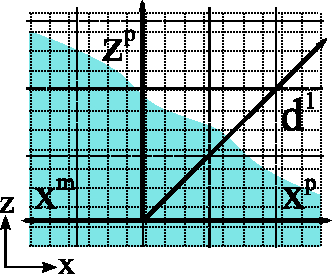
\includegraphics[width=8.2cm]{Figures/chi_opacity_grid}
\caption[Schematic of optical depth calculation]{
Schematic of the optical depth calculation. The fine (dotted) grid
represents the finite difference grid for the fluid evolution; the coarse
(dashed) grid represents the opacity grid for the optical depth calculation.
%The relative resolution of the two grids is consistent with L2.
The blue region in the lower left represents dense fluid in which the neutrino
mean free path is small. For each zone of the opacity grid, we first integrate
five axial rays, excluding the $-z$
axis because of equatorial symmetry; three of these are labeled:
$\rm x^m$, $\rm x^p$, $\rm z^p$.
Then we integrate two additional `most promising' diagonal rays,
lying between the minimum optical depth axis and the two next-to-minimum axes;
one of these is labeled: $\rm d^1$.
}
\label{fig:chi_opacity_grid}
\end{figure}

The most costly part of the leakage scheme is the estimate of the
optical depth.  To compute this, we first interpolate the opacity
(factoring out the $\varepsilon_{\nu}^2$ neutrino energy dependence, as discussed
above) onto a lower resolution 3D grid.  Then we compute
line integrals of this quantity in 7 directions to the computational boundary:
one integral forward and backward on each coordinate axis, excluding $-z$ because of our
grid's reflection symmetry, plus two diagonals based on the `most
promising' of the coordinate directions (see Fig.~\ref{fig:chi_opacity_grid}).
The minimum line integral gives the optical depth.
(More precisely, the optical depth is $\varepsilon_{\nu}^2$ times this integral.)

To test our implementation of the leakage scheme, we have constructed
spherically symmetric configurations of hot gas and compared our
results ($R_{\nu_i}$, $Q_{\nu_i}$, and the optical depth) with those
of GR1D.  We set the neutrino chemical potentials in the same way for
this test to have a clean comparison.  We tried spheres with a range of
central density, temperature,
and $Y_e$, so that some were optically thin and others optically thick. 
As expected, the two codes agreed.

The emission rates also allow us to compute the total neutrino energy
and number luminosity radiated to infinity by performing proper integrals
over $Q_{\nu}$ and $R_{\nu}$.  For the energy luminosity at $r\rightarrow\infty$, $L_{\nu}$,
we multiply the integrand by a redshift factor $\psi_{00}$:  one factor of
$\sqrt{\psi_{00}}$ for the time dilation and one factor for the energy redshift. 
For the integral of $R_{\nu}$, we multiply by a redshift factor of
$\sqrt{\psi_{00}}$.

\section{Trustworthiness and Error}
\label{sec:grhydroconvergence}

\begin{figure}
\centering
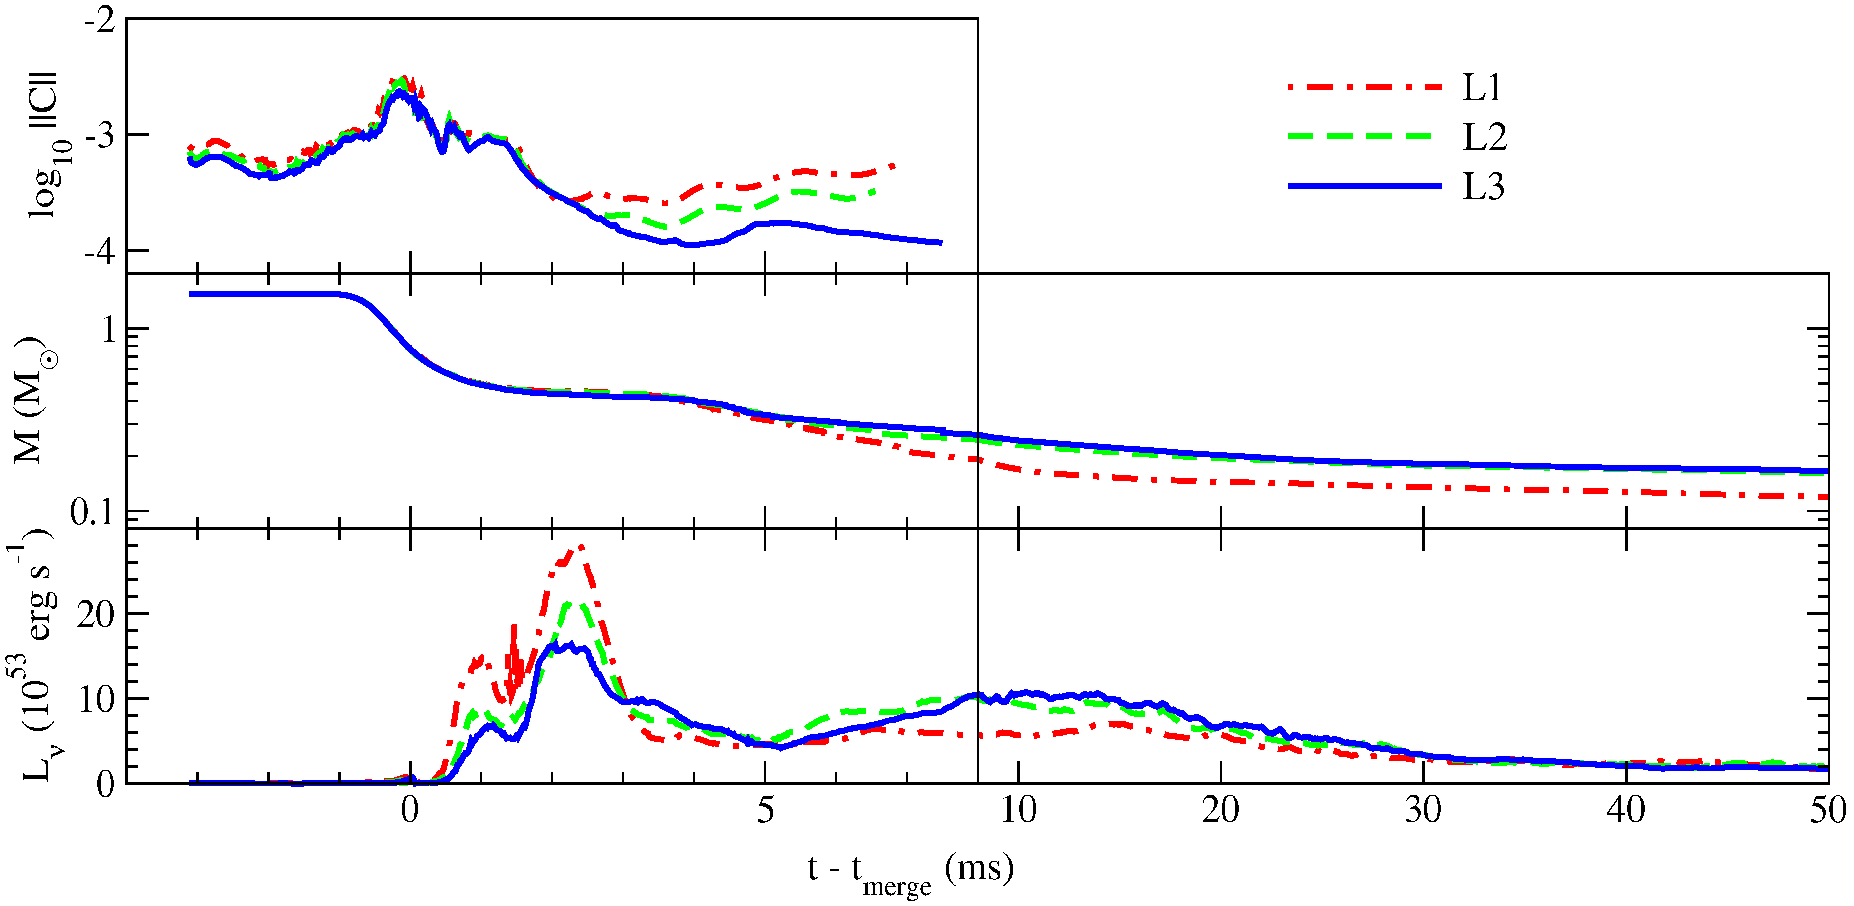
\includegraphics[width=16cm]{Figures/convergence_measures}
\caption[Global convergence measures]{
Global convergence measures,
showing the three resolutions with leakage.
$t_{\rm merge}$ is the time at which 50\% of the rest mass has depleted.
We use different scalings for the time-axis before and after 8~ms
in order to highlight the initial disruption and accretion.
{\em Top panel}: $L^2$ norm of global generalized harmonic constraint
violations (see \citealt{lind2007-gen_harmonic}). We stop tracking this measure at
$\sym7$~ms when we freeze the spacetime metric and begin the Cowling evolution.
{\em Middle panel}: baryonic rest mass remaining on the computational
grid (in units of $M_{\odot}$). The initial decrease beginning at $-1$~ms is
driven by accretion onto the black hole.
The second decrease beginning near $3$~ms is due to matter falling off the outer
bondary of the computational domain.
The disk mass quoted throughout ($M_0 \approx 0.3\,M_{\odot}$) is
the gravitationally bound mass outside the BH at $5$~ms in the L3 evolution,
i.e.\ the mass on the grid minus the instantaneous estimate of the remaining unbound mass
discussed in Section~\ref{sec:outflow}.
{\em Bottom panel}: total neutrino luminosity (in units of $10^{53}\rm\,erg\,s^{-1}$),
as measured at $r \rightarrow \infty$.
}
\label{fig:convergence}
\end{figure}

Our evolution begins with a coordinate separation of 83~km
between the centers of the two compact objects.
The inspiral takes place over 6 orbits (28~ms) and is followed by tidal disruption and merger.
We continue to evolve the spacetime and fluid $\sym7$~ms past merger.
We define `merger' as the time when 50\% of the matter has
depleted, mainly by accretion (at this time, only a small fraction
($<10^{-3}$) has fallen off the outer boundary).
By 7~ms the metric is mostly stationary, but the accretion disk remains
highly dynamic.  The interpolation and communication of the fluid variables
to the spacetime (pseudospectral) grid is the dominant
computational cost during this phase of the evolution,
so continuing to evolve the complete system for many tens of
milliseconds would be prohibitive with the current code.  Instead,
we continue the evolution some 40~ms longer in
the Cowling approximation, that is we evolve the fluid but leave
the spacetime fixed.

The Cowling approximation ignores several effects.
First, it neglects changes in the disk's and the black hole's gravitational pull.
The mass accreted onto the black hole is some two orders of magnitude smaller than
the black hole mass, so this effect is probably unimportant.
Second, it neglects changes in the black hole's spin. We estimate the
change in the Kerr spin parameter through the 40~ms of Cowling evolution by
measuring the change in the angular momentum and mass of the fluid.
If we were to continue evolving the metric, $a^*$ would decay
(from $\sym0.9$) by 2\%, pushing out the radius of the innermost stable
circular orbit by less than 10\% \citep{bard1972-rotating_bh}.
We do not expect this effect to play a significant role in the disk evolution.
Third, the Cowling approximation cannot capture instabilities
due to the disk's self-gravity. However, this should not qualitatively
alter perturbations in the bulk of the disk.
The threshold for gravitational instability can be estimated from Toomre's
criterion:  $Q_T=\kappa c_s/(\pi G\Sigma) >1$ for stability
\citep{safr1960-grav_instability,toom1964-grav_stability}, where $c_s$ is the sound
speed of the disk, $\kappa$ is the epicyclic frequency, 
$\Sigma$ is surface density, and $G$ is the gravitational constant.  For
the disk considered here, the minimum Toomre parameter there is about 20
except for the inner and outer edges.  The small amount of matter in
the outer regions of the grid is not yet in circular orbit equilibrium,
so the stability condition is inapplicable.  At the innermost region
of the disk, $\kappa\rightarrow 0$ at the innermost stable circular
orbit, but here the Cowling approximation does capture
the main orbital instability.
Fourth, the Cowling approximation discards the gravitational
waves caused by the disk's nonaxisymmetry.  For the observed mass
quadrupole variations induced in the disk, gravitational waves will
affect the modes on a timescale $E_{\rm mode}/L_{\rm GW}\sim 10^2$~s
(where $E_{\rm mode}\sim M_0 v^2(\delta\Sigma/\Sigma)^2$ is a
characteristic energy of the spiral waves, and
$L_{\rm GW}$ is the gravitational wave luminosity).
Thus we may safely ignore this effect.
Finally, this approximation `freezes in' any nonaxisymmetric modes present
in the metric when we transition to the Cowling evolution.
We see that the amplitude (normalized to the $m=0$ mode) of the $m\geq1$ modes
in the lapse are below $\sym10^{-3}$ at all radii. We expect this
nonaxisymmetry to feed back into the fluid at the same order of magnitude.
%outside of $r \sim 25\rm\,km$. Inside this radius, it is only slightly above $10^{-3}$.
%Modes with $m>1$ have even smaller amplitudes.
%Note that a mode amplitude of $10^{-3}$
%is more than two orders of magnitude below that of the density perturbations that form
%at late times in the disk (perturbations which we examine in Section~\ref{sec:disk}).

To check the accuracy and robustness of our results, we evolve
the merger at 3 resolutions, which we label 'L1',
'L2', and 'L3'. See Table~\ref{tab:resolutions} for a
summary of the resolutions.  Since the
spectral evolution uses adaptive meshing, the number of colocation
points changes significantly over the course of an evolution, so
we report average resolutions.  The actual numbers of stored fluid
grid points are half those shown in the table, since each stored number
gives the fluid variables at a point below and a point above the
equator, following our assumption of equatorial reflection symmetry. 
After tidal disruption, the coordinate system of our fluid grid
is driven nonuniformly to higher resolution close to the black hole.
Our high resolution corresponds to a fluid grid spacing of $\sim$160~m during
inspiral and about 0.7~km vertical / 2~km radial in the inner
disk after merger.

\begin{table}
  \centering
  \begin{tabular}{ l l l l l }
    \toprule
                    &                             & L1        & L2        & L3 \\
    \midrule
    $N$ gridpoints  & spectral domain             & $70^3$    & $75^3$    & $87^3$ \\
                    & hydro domain                & $120^3$   & $140^3$   & $160^3$ \\
    \midrule
    $\langle dx \rangle$ (km) & early: star       & 0.21      & 0.18      & 0.16 \\
                    & late: inner disk (vert/rad) & 0.9 / 2.7 & 0.8 / 2.3 & 0.7 / 2 \\
    \bottomrule
  \end{tabular}
  \caption[Summary of simulation resolutions]{
    Summary of numerical resolutions. $N$ is the total number of gridpoints in the
    evolution domains. $\langle dx \rangle$ is the average grid spacing on the hydro
    domain, calculated in evolution coordinates.
  }
  \label{tab:resolutions}
\end{table}

In addition to the convergence tests, we perform one merger, at the
L1 resolution, without neutrino leakage.  We label this
run `L1no$\nu$'.  Comparing L1no$\nu$ to L1 lets us isolate
the effects of the neutrinos on the fluid.

\begin{figure}
\centering
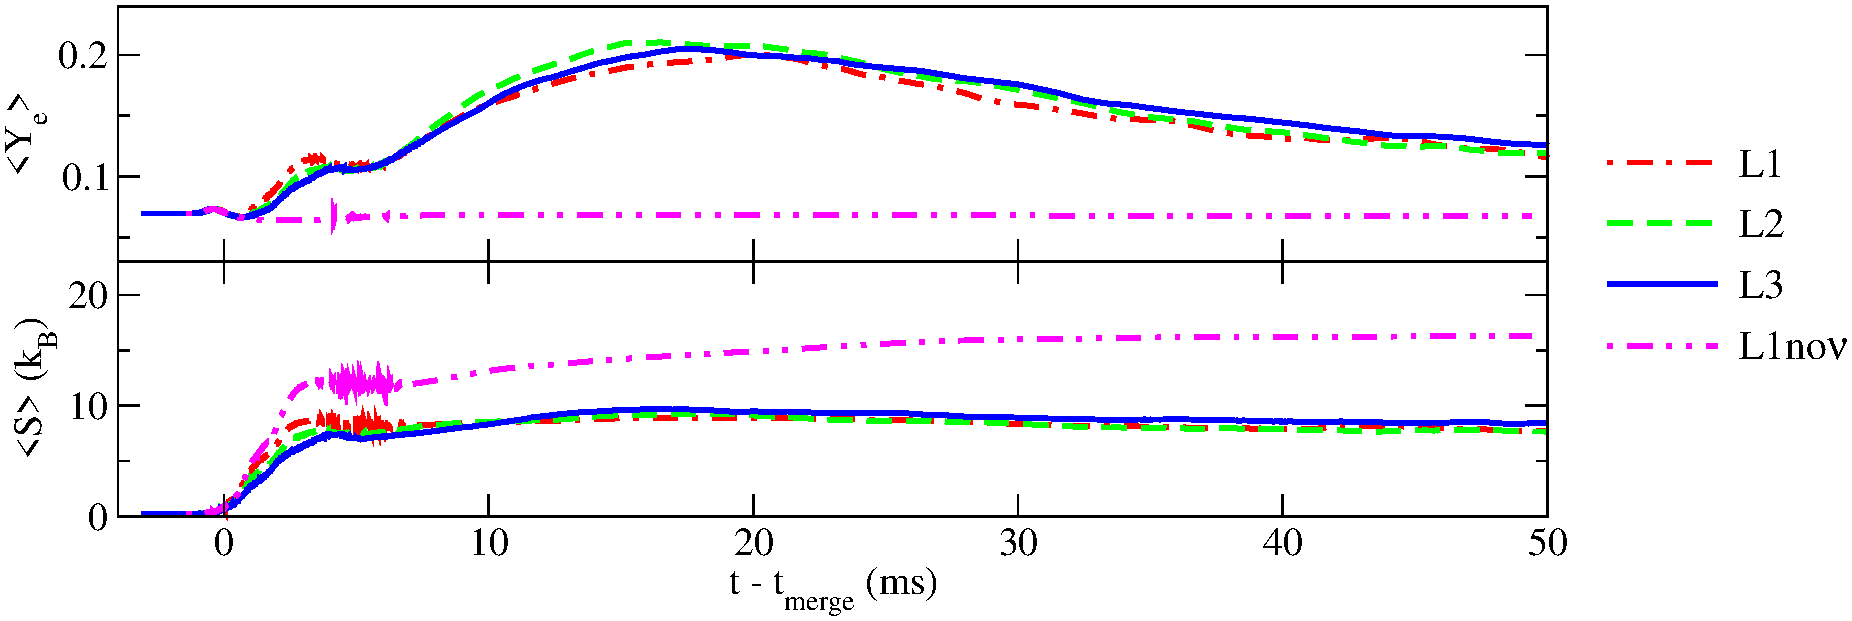
\includegraphics[width=16cm]{Figures/global_measures}
\caption[Secular chemical and thermal evolution of the disk]{
Secular chemical and thermal evolution of the disk for the three resolutions
with leakage, and also L1no$\nu$.
{\em Top panel}: mass-weighted average of the electron fraction.
In the L1no$\nu$ evolution, $Y_e$ simply advects with the flow.
The early decreases at 0~ms and 3~ms are due to the major mass loss episodes:
initial accretion, and loss of the tidal tail from the outer boundary.
{\em Bottom panel}: mass-weighted average of the entropy, in units of
$k_B\rm\,baryon^{-1}$.
}
\label{fig:globalevolution}
\end{figure}

In Figures~\ref{fig:convergence} and~\ref{fig:globalevolution},
we show the evolution of several main global quantities for all runs. 
Comparing resolutions allows us to discern
which evolution features are robust and which are numerical artifacts. 
For example, the neutrino luminosity ($L_{\nu}$) spikes 2~ms after merger,
but this feature appears to converge away as resolution is increased.
Volume renderings of the fluid (see an equatorial slice in Fig.~\ref{fig:disruptionsnapshots})
show that at these times, some of the nuclear matter is spread in
a thin tidal tail which is underresolved at low resolutions. The luminosity
at later times comes from the much better-resolved disk, and we see
good agreement between the higher resolutions on $L_{\nu}$ after
about 5~ms.
Figure~\ref{fig:convergence} reveals that the rest mass
of L1 at late times differs from that of the higher resolutions significantly
more than the high resolutions differ between themselves.
By 10~ms this difference has settled to about 30\%.
The reason for this is that resolution L1 generates a hotter, fatter,
lower-density disk.
%Even as early as $t=0.5$~ms, when the maximum density of the disrupted stars
%is $\sym5\times10^{13}\rm\,g\,cm^{-3}$, the behavior of the resolutions
%can be seen to diverge (with L1 consistently lower
%in density and higher in entropy than L2/L3).
%By $t=2$~ms, L1 has a consistently higher outflow than L2/L3.
%At late times, when the disk has settled in cowling, it's clear
%that L1 is outflowing less than L2/L3 (probably because the regridder
%sent the outer boundary out further for L1 in the early merger.)
The puffed-up disk drives more of its matter off of our computational domain,
an effect that we can already see in outflow measurements by 2~ms after merger
(see Section~\ref{sec:outflow}).
Finally, in Fig.~\ref{fig:globalevolution}, we again see that the different
resolutions agree well on the post-merger composition and entropy,
giving us confidence that these are roughly correct, though
strict convergence is lacking.  Given the strong shocks and
turbulent-like behavior in the disk, this is unsurprising.
However, comparing the leakage runs to L1no$\nu$, we see that the secular
neutrino effects are much larger than the differences between resolutions.

\section{Dynamical Outflows}
\label{sec:outflow}

In a BHNS merger, matter expelled at high velocity
may ultimately become unbound from the central gravitational potential.
In addition to enriching the interstellar medium with r-process elements
\citep{latt1974-bhns_ejecta,frei1999-r_process,arno2007-r_process,koro2012-r_process},
this nuclear matter may emit an electromagnetic signal.
The radioactive nuclei formed in the neutron-rich fluid
quickly fission, emitting high-energy beta- and gamma-radiation.
This heats the ejecta, which becomes optically thin on an expansion
timescale (days to weeks), and radiates thermalized photons, producing
an isotropic kilonova (or `macronova', see
\citealt{li1998-transients,robe2011-transients,metz2012-most_promising,ross2012-ejecta,
pira2013-em_counterparts,kase2013-opacities,niss2012-end_to_end})
at optical, or perhaps infrared, wavelengths, depending on the highly-uncertain
opacity properties of the material \citep{kase2013-opacities}.

Additionally, the high-velocity ejecta form a blast wave in the circumbinary medium.
At the shock front, magnetic fields amplify and accelerate electrons and positrons,
thus emitting synchrotron radiation.
This radio emission continues for a deceleration timescale (months to years)
dependent upon the density of the surrounding medium
\citep{metz2012-most_promising,naka2011-radio,pira2013-em_counterparts,niss2012-end_to_end}.

These transient electromagnetic signals are of sufficient interest
to warrant a thorough examination of any ejecta in our simulation.
There are two dominant conveyers of ejecta in BHNS mergers:
tidal tails and accretion disk winds.  In this simulation, most of
the unbound mass is produced by the tidal tail.  A smaller amount is
ejected in a plume during the early merger phase, as the infalling gas stream
collides and shocks with itself. Also a small amount of outflow from the late disk
is observed, but at low densities where numerical errors can introduce
spurious acceleration and heating of the fluid.
Note that this simulation ignores some effects that could drive
strong winds (e.g. neutrino heating) and does not evolve long enough to
see some others (e.g. large-scale He recombination).
Below we review previous results, describe the formation of the tidal tail,
describe our method of analyzing the ejecta, and finally report measures of
its mass ($M_{\rm ej}$), kinetic energy ($E_{\rm ej}$),
distribution of velocities, and composition ($\langle Y_e \rangle_{\rm ej}$).

There are a number of recent studies examining ejecta from
binary neutron star mergers (e.g.\ \citealt{ross2012-ejecta,hoto2013-ejecta}),
high-eccentricity mergers (e.g.\ \citealt{step2011-eccentric,east2012-eccentric,east2012-dynamical_capture}),
and mergers including magnetic fields (e.g.\ \citealt{chaw2010-magnetized}).
But here we survey results from low-eccentricity, nonmagnetized, BHNS studies
to emphasize the influence of black hole spin.
\cite{latt1974-bhns_ejecta} made semianalytic estimates in a Schwarzschild spacetime.
They found $M_{\rm ej} \sim 0{\rm\,\,to\,\,}0.14\,M_{\odot}$ for stars that disrupt
close to the black hole; no mass is ejected from stars that disrupt far away.
\cite{ross2012-ejecta} simulated two cases of $q\sim4$ and $q\sim7$ in a
Newtonian potential. He found $M_{\rm ej} \lesssim 0.05\,M_{\odot}$.
Relativistic simulations have characteristically yielded more
conservative ejecta estimates.
Notably, high mass-ratio, compact neutron star, low black hole spin systems do not even
disrupt. (See \citealt{pann2010-disk_mass} and \citealt{fouc2012-disk_mass} for phenomenological models
covering this parameter space.)
In an excellent study focused on unique signatures from BHNS merger ejecta,
\cite{kyut2013-ejecta} simulated a suite of tens of mergers
with mass ratios of $q=3$ to $7$ and prograde BH spins up to $a^{*}=+0.75$.
They showed $M_{\rm ej} \sim 0.01\,M_{\odot}$ to $0.07\,M_{\odot}$, with more matter ejected
if the EOS is stiff.
Recently, \cite{fouc2013-compactness_and_spin} simulated several
mergers of $q=7$, with large BH spins of $|a^{*}|=0.9$ varying in inclination.
In cases of aligned spin and orbital angular momentum, they found ejected
masses of $M_{\rm ej} \sim 0.09\,M_{\odot}$.
Finally, in a study with nearly-extremal BH spin, \cite{love2013-bhns_high_spin} found
$M_{\rm ej}$ could be as high as $0.3\rm\,M_{\odot}$.
It appears, then, that for BHNS systems, one parameter region of interest for significant ejecta
may be the parameter region of high spin.

In the present simulation, we see a large tidal tail form just before merger.
About two orbits before merger ($t=-3$~ms) the coordinate separation
of the two centers of mass has decayed to
$40$~km and the neutron star has become extremely distorted.
After another revolution ($t=-1.5$~ms) the separation has decayed to $25$~km,
the star overflows its Roche lobe, and it begins to accrete onto the black hole.
A tidal tail has already formed from the trailing edge of the star,
extending outward and lagging an orbit behind the core.
At $t=0$, the core falls into the black hole.
Over the next 3~ms the tidal tail sweeps out and
away from the black hole (see Fig.~\ref{fig:disruptionsnapshots}).
We follow the tail by periodically resizing our computational domain outward to
a radius of $\sym400$~km, where we allow the tail to fall off of the grid.
From its formation until its exit, the tidal tail is evolved on the computational domain
for $\sym5$~ms.

\begin{figure}
\centering
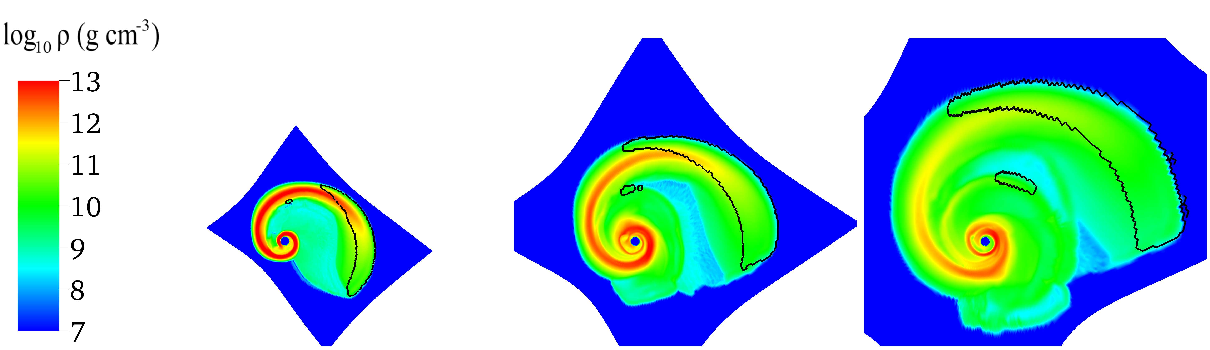
\includegraphics[width=16cm]{Figures/rho_unbound_1ms_2ms_3ms}
\caption[Time sequence of dynamical ejecta]{
Equatorial slices of rest density from L3
during disruption and tidal tail formation at 1, 2, and 3~ms after merger
(from left to right).
The unbound material is outlined in black. The field of
view is fixed in all panels, so that each
has a scale of approximately $680\times680\rm\,km^2$.
The computational grid expands with the tail until it covers a circle of
radius $\sym400$~km (in our asymptotically flat evolution coordinates)
at which we remove matter from the grid. Note that we distort the
coordinate map between the fundamental evolution frame and the
frame in which the finite difference grid is uniform
in order to concentrate resolution near the black hole (see \citealt{duez2009-3d_eos_advection}).
}
\label{fig:disruptionsnapshots}
\end{figure}

For a stationary spacetime, $u_t$ (the projection of the four-velocity along
the timelike Killing vector field) is a constant of motion for geodesics. 
Assuming the space is also asymptotically flat, $u_t$ gives the Lorentz
factor ($\gamma=-u_t$) of the particles as they escape to infinity.  To the
approximation that the spacetime is settled and that pressure is dynamically
negligible, $u_t$ will be a constant along fluid parcels, and matter with
$u_t<-1$ may be flagged as unbound. Neither approximation is strictly true,
but both become better satisfied as the outflow expands outward away from
the dynamical region and decompresses to low pressures.  Thus, $u_t$ of
fluid elements in the tail, and the total amount of unbound material in
the tail, should become constant as the tail expands.  If this settling
happens before the tail leaves the computational grid, meaningful statements
about the amount of outflow and its asymptotic velocity distribution can
be made.

We integrate the mass satisfying the unboundedness
condition $u_t<-1$ over times from $t \sim 0$~ms, just as
the tidal tail is forming, to $t \sim 7$~ms, after the tail has entirely fallen off
the computational domain. We mask out regions within
$50\,M_{\odot}$ (73~km) of the BH in the evolution coordinates.
At this distance the Newtonian gravitational
potential is $M_{\rm BH}/r \lesssim 0.15$.
The integral of total mass ejected is robust against
30\% variations in the mask radius.
Furthermore, our velocity cap (see Sec. \ref{sec:Methods}) is only applied
at densities below $\sym 10^{8}\rm\,g\,cm^{-3}$ during this epoch, a full 3
orders of magnitude below the maximum density in the tail.

We check the validity of our assumption that the spacetime has become
stationary by estimating the timescale that $u_t$ will change due to changes
in the metric.  For a nonrelativistic geodesic, the leading order term for
the time derivative is $\dot{u}_t\approx \psi_{tt,t}$, so the timescale on which
metric nonstationarity can produce a large relative change in energy is
$\approx (-u_t-1)/\dot{u}_t$.  This is $\sim$~50~ms to 1~s for our ejecta
when near the edge of the computational domain.  On the other hand, the
metric is rapidly settling as the gravitational wavetrain overtakes the
ejecta, and $\dot{u}_t$ drops by an order of magnitude in a few ms.  Thus,
the ejecta energy is not expected to change by a large amount.  However,
tracking the ejecta for an extra few milliseconds would significantly
reduce this source of error, an important consideration for future
simulations.

\begin{figure}
\centering
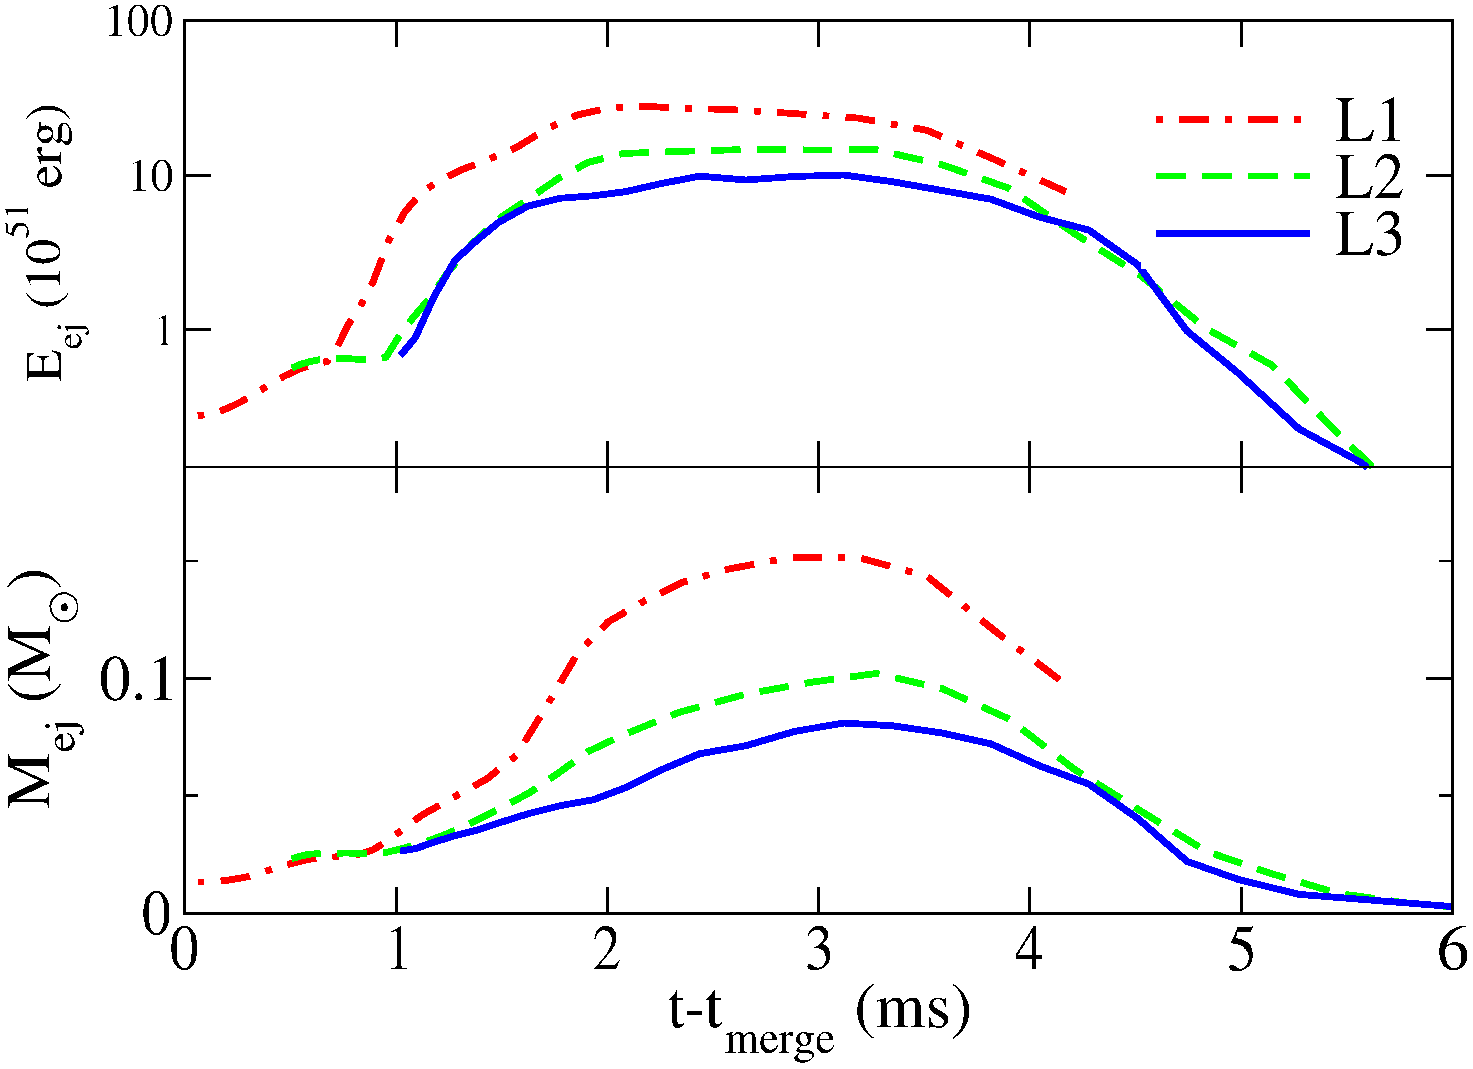
\includegraphics[width=9cm]{Figures/unbound_mass_and_energy_over_time}
\caption[Unbound matter mass and kinetic energy]{
Integrals of the unbound fluid on the grid.
{\em Top panel}: total asymptotic kinetic energy.
{\em Bottom panel}: total rest mass.
For both integrals a sphere of 73~km near the black hole was masked out.
The drop-off after 3~ms is due to the loss of matter through
the outer boundary.
}
\label{fig:ejecta_mass_and_energy}
\end{figure}

Measures of $M_{\text{ej}}$ and $E_{\text{ej}}$ from the three resolutions
are shown in Fig.~\ref{fig:ejecta_mass_and_energy}, where we have calculated the total integral
over unbound matter on the grid.
This raw measure increases early as a growing amount of material
is flung out from the disk and exits the masked region.
In addition to the tail, volume renderings of the unbound matter reveal the existence of
a plume of outgoing matter ejected above the equatorial plane, of lower density than the tidal tail visible
in Fig.~\ref{fig:disruptionsnapshots}.  This second outflow is produced during
the merger, perhaps by the shock waves in the infalling matter. 
The most energetic matter in this plume begins to fall off the
computational domain after 2.5~ms, whereas the dense tidal tail begins to fall off
after 3~ms. Therefore, we use the peak values of mass and kinetic energy in
Fig.~\ref{fig:ejecta_mass_and_energy} as conservative estimates.
We use Richardson extrapolation to derive uncertainties from the highest two resolutions,
and we assume $2^{\rm nd}$ order convergence, though Fig.~\ref{fig:ejecta_mass_and_energy}
indicates approximately $6^{\rm th}$ order covergence. This method gives
$M_{\rm ej}= 0.08 \pm 0.07 \,M_{\odot}$, and
%A 2nd-order convergence estimate from L2-L3, for which (dx_2/dx_3)^2=1.3, M_ej_3 = 0.08 Msun,
%dm_ej=0.02Msun, yields $M_{\text{ej}}= 0.08 \pm 0.07 \,M_{\odot}$.
%Or $M_{\rm ej}= 0.08 \pm 0.02 \,M_{\odot}$, from difference between L2-L3
$E_{\rm ej} = 10 \pm 17 \times 10^{51}$~erg.
%$(dx_{\rm L2}/dx_{\rm L3})^2 \approx 1.3$,
%$E_{\rm ej,L3} = 10$~B, $dE_{\rm ej,L2,L3}=5$~B, so
%$\Delta E_{\rm ej} \approx 5\,{\rm B}/(1.3-1) \approx 17$~B.
%A 6th order estimate would give $\Delta E_{\rm ej} \approx 4$~B.
%Or $E_{\rm ej} = 10 \pm 5 \times 10^{51}$~erg, from difference between L2-L3.
These errors are upper bounds which are probably large overestimates.
Nonetheless, even at our highest resolution, the tail is poorly resolved:
at $\sym70$~km wide, it is covered by $\sym15$ grid cells. This is a common limit
of grid-based methods; smoothed-particle hydrodyanmics methods neatly overcome this
limit, but find their handicap in evolving accurate initial conditions for the tail.

\begin{figure}
\centering
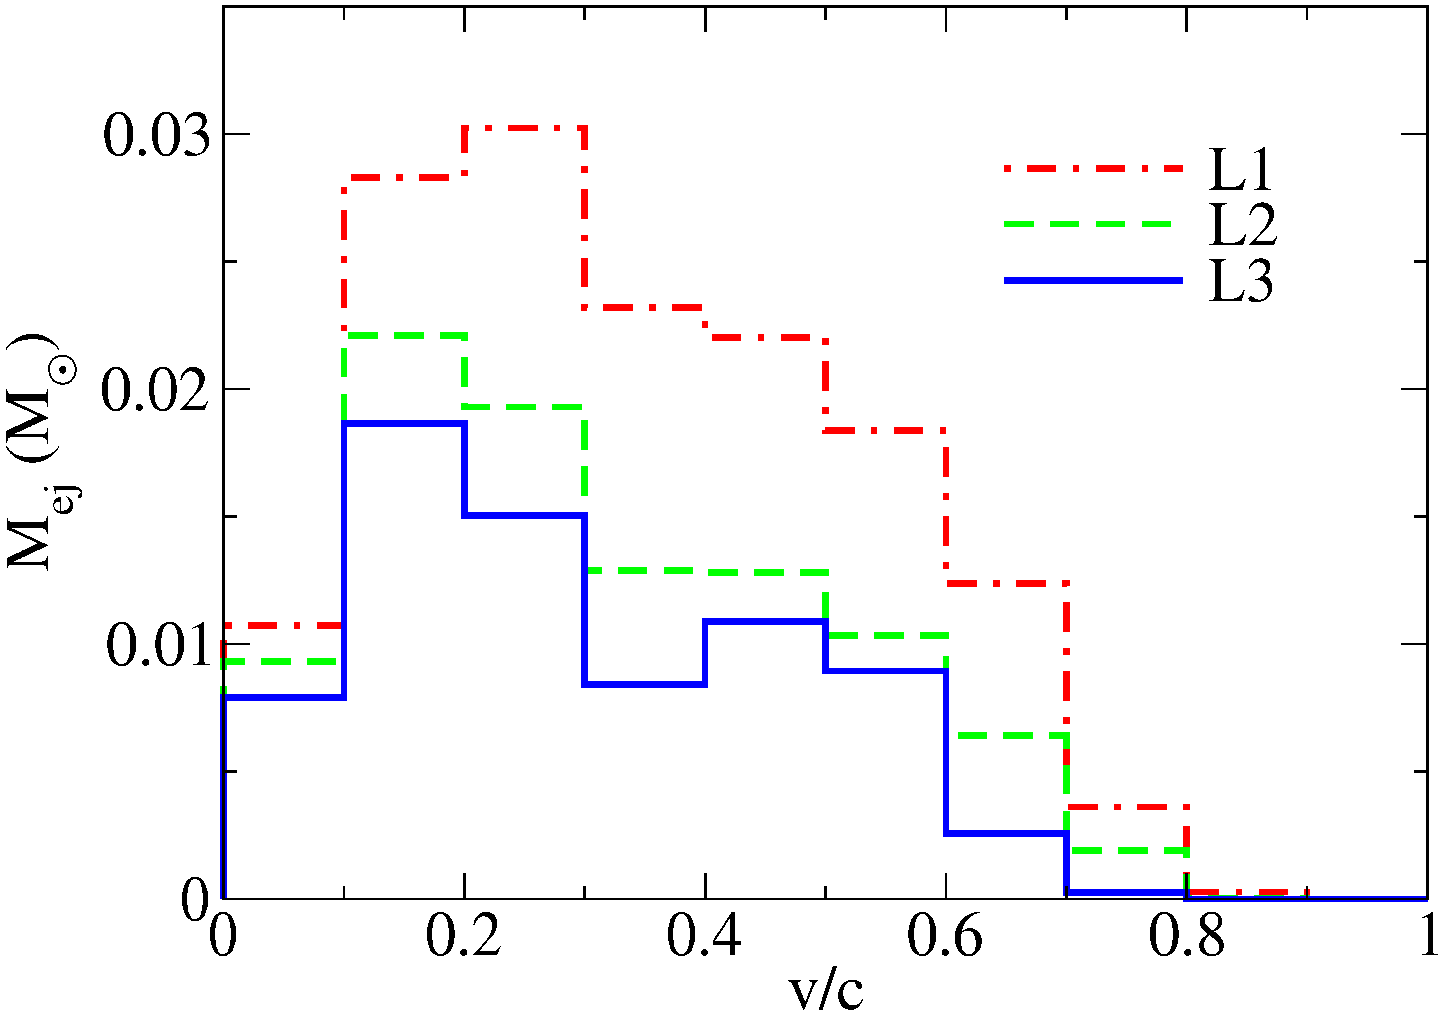
\includegraphics[width=9cm]{Figures/unbound_velocity_histogram}
\caption[Unbound matter asymptotic velocity]{
Unbound rest mass binned by magnitude of the asymptotic fluid velocity.
We show L1, L2, and L3 at $~\sym2.7$~ms, just before the peak in
Fig.~\ref{fig:ejecta_mass_and_energy}.
}
\label{fig:ejecta_velocity_histogram}
\end{figure}

The velocity distribution peaks across all resolutions at $0.2c$, but the dispersion in
velocities is large, with some matter escaping at $v>0.5c$
(see Fig.~\ref{fig:ejecta_velocity_histogram}).
Because average temperatures in the tidal tail are $\sym 1$~MeV as it leaves
the computational domain, the fluid is still in nuclear statistical equilibrium,
so our equation of state is still valid.
The material ejected from the
system is neutron-rich, with average electron fraction
$\langle Y_e \rangle_{\rm ej} \approx 0.1$.
%At $t=1$~ms $\langle Y_e \rangle$ in the tail is near the minimum value allowed by the EOS (0.035).
%But it releptonizes rapidly; by $t=3$~ms, $\langle Y_e \rangle \sim 0.12$.

\section{Accretion}
\label{sec:accretion}

\subsection{Accretion Timescales}
\label{sec:scales}

The density in the accretion disk peaks at a circumferential
radius $r$ of around 50\,km from the black hole, and most of the
disk mass is within 100\,km of the black hole.  At the density
peak, the density is $\rho\approx 10^{12}$g cm${}^{-3}$, the
angular frequency $\Omega$ is around 3\,kHz, and the sound speed $c_s$
is around 0.1$c$.  The disk is hot and
thick:  $H/r\sim c_s/(\Omega r)\sim\frac{1}{3}$. 
The dynamical timescale of the disk is, to order of magnitude,
\begin{equation}
T_{\rm dyn} \sim \Omega^{-1} \sim \frac{H}{c_s} \sim \frac{r}{c_s}\
\sim 1\,\mathrm{ms}.
\end{equation}
Angular frequency decreases with distance from the black hole, so the
orbital period at $r=$120\,km (roughly speaking, the disk's outer edge)
is 10\,ms.  Thus, even this outer region is evolved for several
dynamical times. 
The perturbations in the inner disk rotate at frequencies similar to
the local flow and thus orbit the black hole on millisecond periods. 

The disk has strong entropy gradients in the inner and outer regions,
so disk gas can experience buoyancy forces there on a timescale given by the
Brunt-V\"ais\"al\"a frequency $N_{\rm BV}$,
\begin{equation}
T_{\rm S} \sim \left|N_{\rm BV}{}^2\right|^{-1/2}
=  \left|-\rho^{-1}(\partial\rho/\partial S)_P\,g\cdot\nabla S\right|^{-1/2} \approx 1{\rm\,ms}\ ,
%\left(\frac{\nabla P \nabla S}{\rho^2 (\partial S/\partial\rho)|_P}
%\right)^{-1/2} \sim \mbox{ms},
\end{equation}
where $g=\rho^{-1}\nabla P$ and $S$ is the specific entropy. 

In addition to these dynamical processes, there are secular processes
that alter the disk structure on longer timescales.  One such effect
is the depletion of baryonic mass in the disk. 
The disk's mass is $M_0 \approx 0.3M_{\odot}$ after merger
(see Fig.~\ref{fig:convergence}).
For the first 30\,ms after merger, accretion onto the black hole proceeds at a rapid
rate of $\dot{M}_0 \approx 2\,M_{\odot}\rm\,s^{-1}$.  During this time, the
gas in the outer disk settles into circular orbit, which requires a
transfer of angular momentum from the inner disk.  (See
Section~\ref{sec:disk} for a fuller discussion of the disk's angular
momentum evolution.)  The transport of angular momentum away from the inner
disk by spiral density waves drives accretion onto the black hole. 
Eventually, the high-density middle region of the disk settles to
equilibrium, but dynamical, nonaxisymmetric distortions persist
near the disk's inner and outer edges (also discussed in
Section~\ref{sec:disk}).  Spiral waves thus travel outward and drive
a reduced rate of accretion throughout the simulation.  After 30\,ms, the
accretion rate has dropped by nearly an order of magnitude.  At
these late times, disk mass is also lost to a weak outflow from the inner
disk at a comparable rate to the accretion into the black hole.  Combining
these effects, we can define a mass depletion timescale
\begin{equation}
T_{\rm dep}\sim \frac{M_0}{\dot{M}_0}\gtrsim 0.2{\rm\,s}\ .
\end{equation}

The disk's thermal evolution is driven by shock heating, compression,
advection of heat into the black hole, and radiative cooling. 
The disk's thermal energy is defined as
\begin{equation}
E_{\rm thermal}=\int \rho_*[\epsilon - \epsilon_{\rm cold}(\rho,Y_e)]d^3x,
\end{equation}
where $\epsilon$ and $\epsilon_{\rm cold}(\rho,Y_e)$ are the actual
specific internal energy and the specific internal energy at the
lowest temperature in the EOS table, for which the gas is degenerate. 
We find $E_{\rm thermal}\approx 10^{52}\rm\,erg$. 
The total neutrino luminosity is $L_{\nu} \sim 10^{53\text{--}54}\rm\,erg\,s^{-1}$. 
Therefore, the cooling timescale due to neutrinos is
% L_nu conversion factor = 3.8e59 or 2.62e-60
\begin{equation}
T_{\rm cool}\sim \frac{E_{\rm thermal}}{L_{\nu}} \approx 10{\rm\,ms}\text{--}100{\rm\,ms}.
\end{equation}
It is important to remember that the disk is partly pressure-supported.
Thus radiative energy loss
may come from the potential energy reservoir via disk contraction,
in addition to the more obvious thermal energy reservoir via disk cooling.
Indeed we find that evolving without neutrino cooling
leads to a disk that is not only hotter but also much more extended and
less dense.  The timescale for composition change
is $N_e/R_{\nu}$, where $N_e$ is the number of electrons in the disk and
$R_{\nu}$ is the total net lepton number change rate due to neutrinos. 
This is initially also about
10~ms.  Then, 20~ms after merger, balance between $\nu_e$ and $\overline{\nu}_e$
emission is roughly achieved, and the
composition subsequently changes more slowly.   Thus, the neutrino emission
significantly influences the energy and composition of the disk over its
lifetime.

\subsection{Accretion Disk: Dynamical Equilibrium and Stability}
\label{sec:disk}

\subsubsection{Disk Formation}

As can be seen from Fig.~\ref{fig:globalevolution},
as the accretion stream collides with itself, shocks heat
the gas for roughly one millisecond, until the density-averaged
entropy settles at $\sym 8\,k_B\,\rm baryon^{-1}$. 
A hot accretion disk forms in the vicinity of the black hole.  In
Fig.~\ref{fig:disksnapshot}, we show density snapshots
of the disk at a representative time $\sym 30$~ms later,
and in Fig.~\ref{fig:thickness}, we show
azimuthally averaged equatorial density as
a function of circumferential radius.  The maximum density remains at a fairly
steady level of $\sym 10^{12}\rm\,g\,cm^{-3}$.  As shown in the bottom
panel of Fig.~\ref{fig:thickness}, the densities and temperatures
are sufficient to render the interior of the torus optically thick
to all species of neutrinos, with optical depths (averaged over
neutrino energy) of order 10.

\begin{figure}
\centering
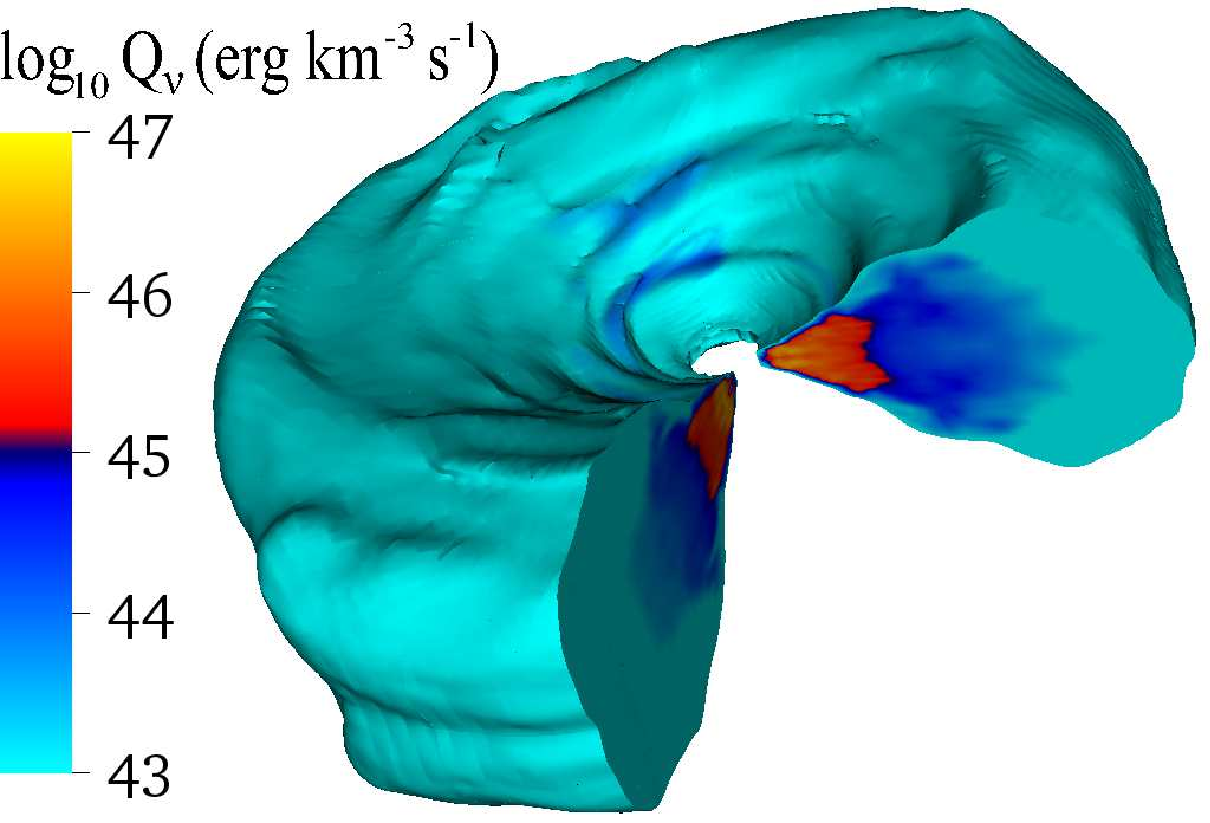
\includegraphics[width=9cm]{Figures/3D-Q0phys_meridional}
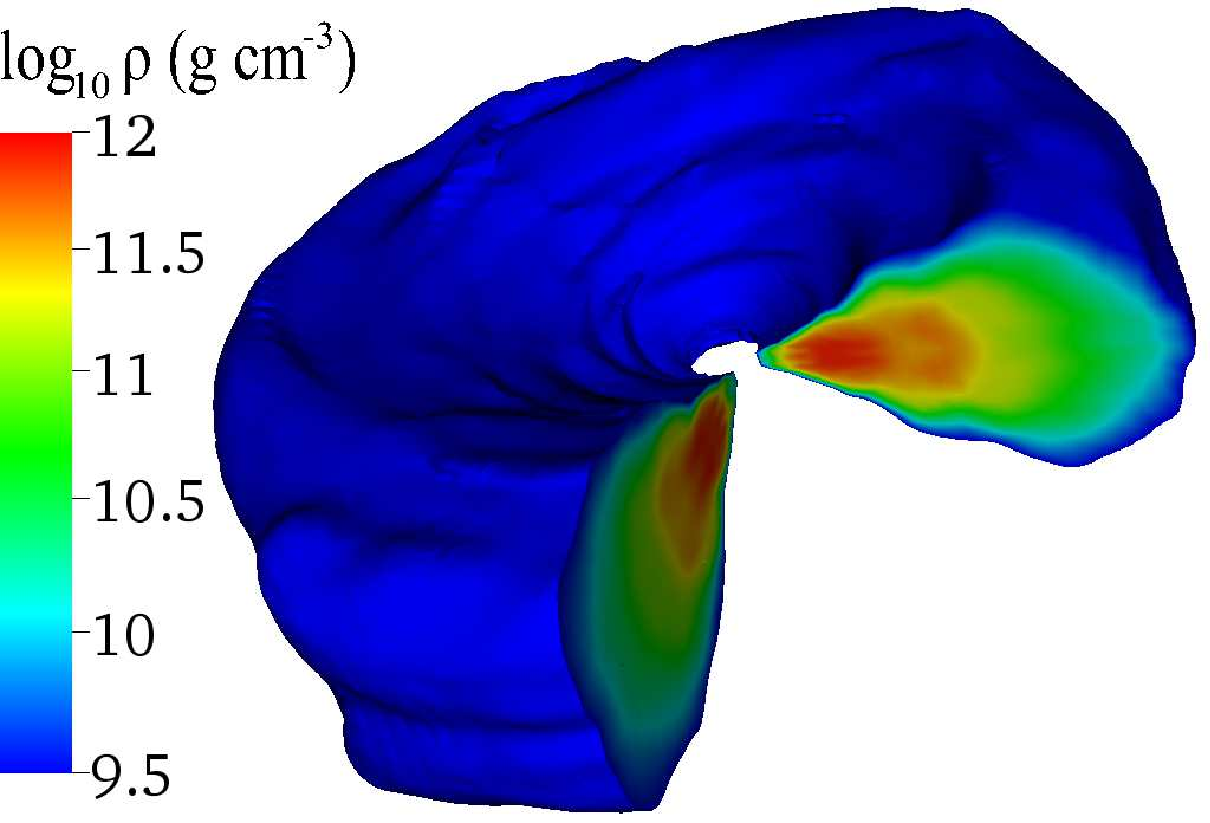
\includegraphics[width=9cm]{Figures/3D-rho0phys_meridional}
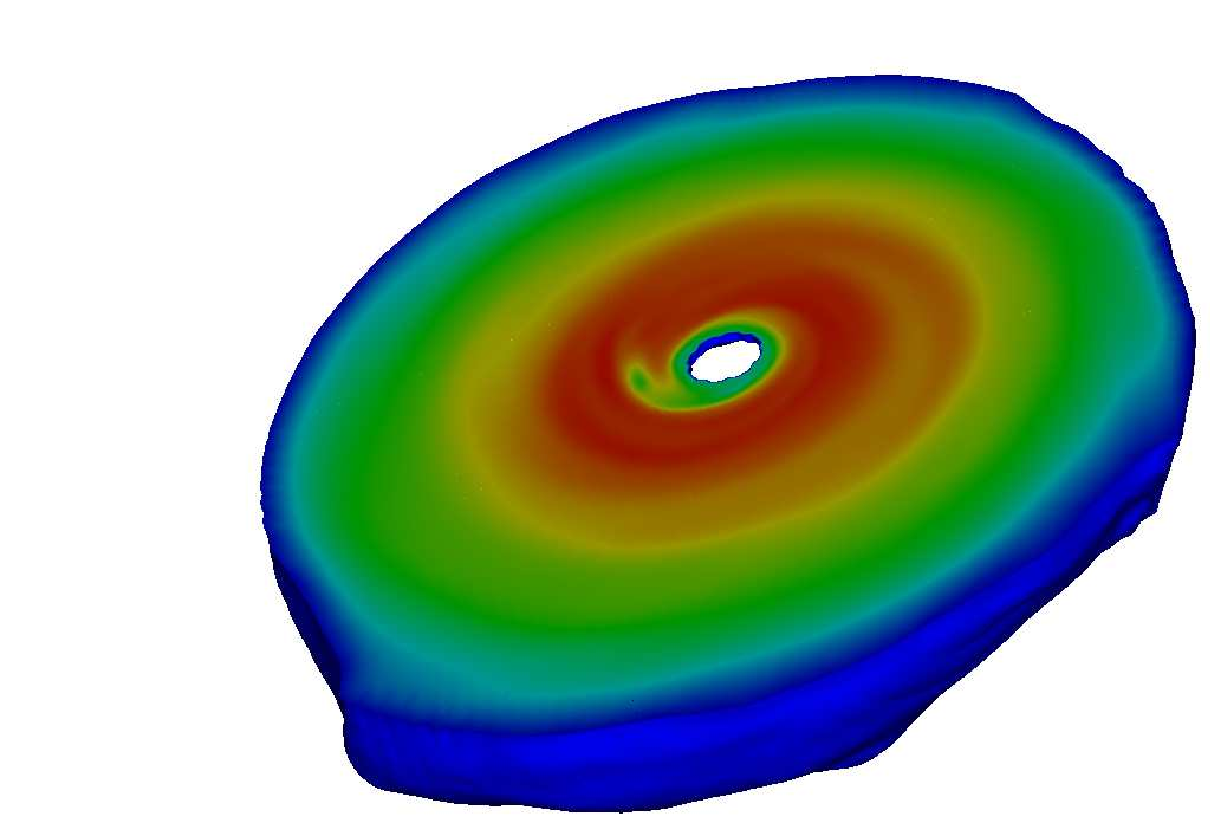
\includegraphics[width=9cm]{Figures/3D-rho0phys_equatorial}
\caption[Three-dimensional colorplots of disk density and neutrino energy losses]{
Three-dimensional distribution of neutrino energy loss and fluid density
from L3, 30~ms after merger, depicted in evolution coordinates at a slanted view.
{\em Top panel}: effective local neutrino power, $Q_{\nu}$ (no redshift applied),
summed over all species (in units of $\rm erg\,km^{-3}\,s^{-1}$).
{\em Middle and bottom panels}: meridional and equatorial slices of
density in the fluid rest frame. The equatorial slice reveals a spiral mode.
In all three panels, densities below $10^{9.5}\rm\,g\,cm^{-3}$ have been masked out
to show the structure of the disk. The disk radius and half-thickness
are 110~km and 45~km, respectively.
}
\label{fig:disksnapshot}
\end{figure}

\begin{figure}
\centering
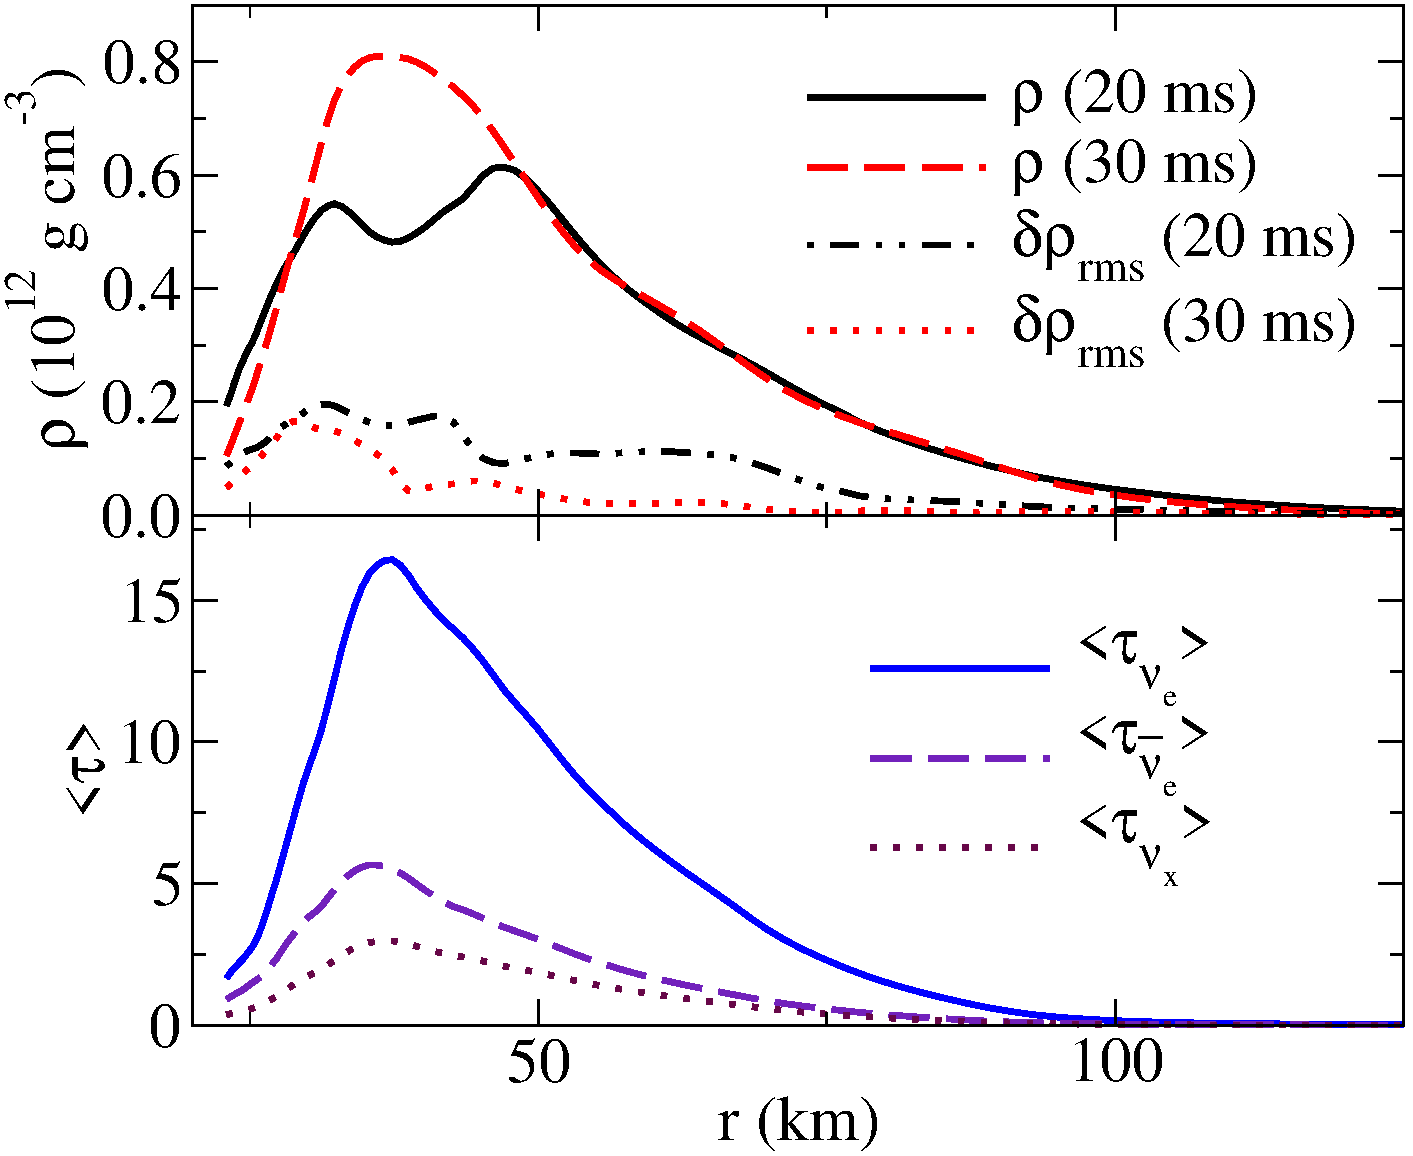
\includegraphics[width=9cm]{Figures/thickness}
\caption[Radial profiles of disk density and opacity]{{\em Top panel}: azimuthally-averaged profiles of the
density $\rho$ together with its RMS deviation from axisymmetry,
$\delta\rho_{\rm rms}\equiv \langle(\rho-\langle\rho\rangle)^2\rangle^{1/2}$,
plotted as functions of the circumferential radius
at the equator $r$.  Values for 20~ms and 40~ms after merger are shown.  
{\em Bottom panel}: density-weighted azimuthal and vertical average of
the energy-averaged neutrino optical depth for each species of neutrino,
computed 40~ms after merger.}
\label{fig:thickness}
\end{figure}

The disk is initially extremely distorted and nonaxisymmetric.  For
a completely stable disk, one would expect the inner regions, where
the dynamical timescale is shortest, to settle to a stationary
axisymmetric state before the outer regions---as was seen, for example,
in a recent BHNS $\Gamma$-law EOS merger carried out with the same
code~\citep{love2013-bhns_high_spin}.  (Unfortunately, we have not performed
any $\Gamma$-law EOS merger simulations with similar mass ratio and
black hole spin to the present case, so no proper comparison can be
made.)  We see instead that it is only the
middle disk that settles to an approximately axisymmetric state after
about 30\,ms. 
In the inner disk, very close to the black hole, clear, order unity
deviations from axisymmetry in the form of trailing one-armed spirals
persist throughout the evolution (see the bottom panel in Fig.
\ref{fig:disksnapshot}).  These perturbations appear at the
disk's inner edge, rotate at roughly the rate of the local fluid
($\sym\rm ms$ periods), expand outward and dissipate, and then reform
many times during the disk evolution.  Such behavior suggests that
a fluid instability may be preventing the disk from promptly settling.

\subsubsection{Disk Equilibrium}

Further insight into the structure of the disk comes from the profiles
of the specific orbital energy ($E\equiv-u_t-1$) and angular momentum
($L=-u_{\phi}/u_{t}$) shown in Fig.~\ref{fig:equilibrium}.  Each panel
includes three curves.  One is the actual $E$ or $L$ profile, measured
on the equator and averaged over azimuthal angle.  Another is the
`Keplerian' $E$ and $L$, the values that would be found for geodesic
equatorial circular orbit given the evolved spacetime metric of the
system.  The geodesic circular orbits are those for which
$\nabla_{\vec{u}}\vec{u}=0$.  These curves thus include the effects of
the disk's self-gravity (at least, as it was at the beginning of the
Cowling evolution) but disregard pressure forces.  We see that the angular
momentum profile, for instance, is much shallower than would be found
for an equilibrium thin (geodesic) disk.  Finally, we include
`equilibrium' curves, the $E$ and $L$ for equilibrium circular
orbit given the existing metric, density, and pressure.  These
are orbits for which $\nabla_{\vec{u}}\vec{u}=-\vec{\nabla}P/(\rho h)$. 
In regions
where deviations from equilibrium are nonlinear, one must take care
in identifying these curves with the true equilibrium about which the
disk is perturbed, since $m=0$ perturbations in the pressure will
feed back into the equilibrium condition.  Given this qualification,
we see that the highest-density regions do appear to be in equilibrium
in an angle-averaged sense.  The outer disk has sub-equilibrium
angular momenta, so the gas remains in eccentric orbit.  Interestingly,
the energy and angular momentum increase dramatically at the inner
edge of the disk.  This feature is not present in the geodesic curves,
but it is in the equilibrium curves, indicating that it is a consequence
of a sharp pressure gradient near the inner edge of the disk.  Below,
we will consider the effect of these gradients on the expected stability
of the disk.  The high
energies in the inner disk would make it easy to generate an outflow there. 
We do indeed observe some mass ejection from the inner disk, but at densities
too low to be reliably modeled by our code.

The difference between the actual and equilibrium energy curves provides a
measure of the mode energy, again, to the extent that equilibrium curves
can reliably be computed from an incompletely settled pressure profile: 
$E_{\rm mode}\equiv \int \rho_*(E-E_{\rm equilibrium})d^3x$.  As shown in
Fig.~\ref{fig:mode},
the mode energy
is positive but decreases during the early, rapid accretion, phase.  Then
it settles and even shows episodes of growth, which may indicate that
instabilities are stimulating these modes.

\begin{figure}
\centering
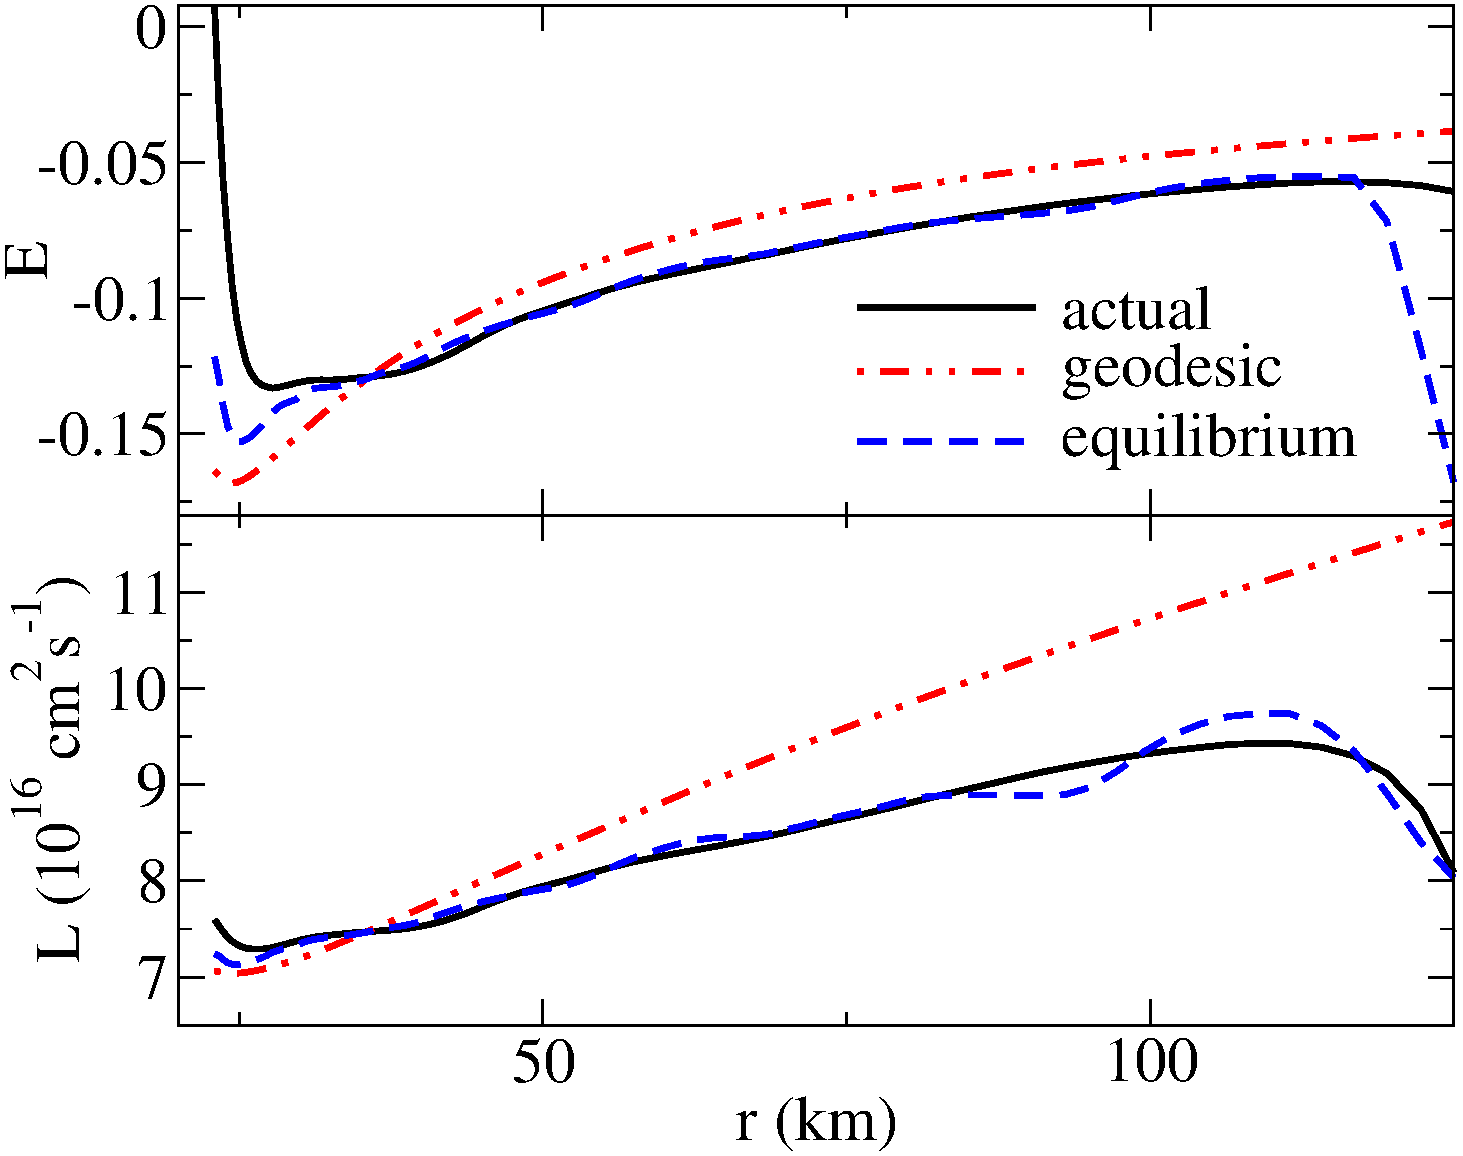
\includegraphics[width=9cm]{Figures/EandL}
\caption[Radial profiles of disk orbital energy and angular momentum]{
Energy and angular momentum of the disk 40~ms after merger.
{\em Top panel}: azimuthally-averaged equatorial orbital energy
$E\equiv-u_t-1$.
{\em Bottom panel}: azimuthally-averaged angular momentum
$L=-u_{\phi}/u_{t}$.
In addition to $E$ and $L$ for the
actual flow, we include values for circular orbit geodesic motion and
circular orbit equilibrium (i.e. including pressure) motion.
}
\label{fig:equilibrium}
\end{figure}

\begin{figure}
\centering
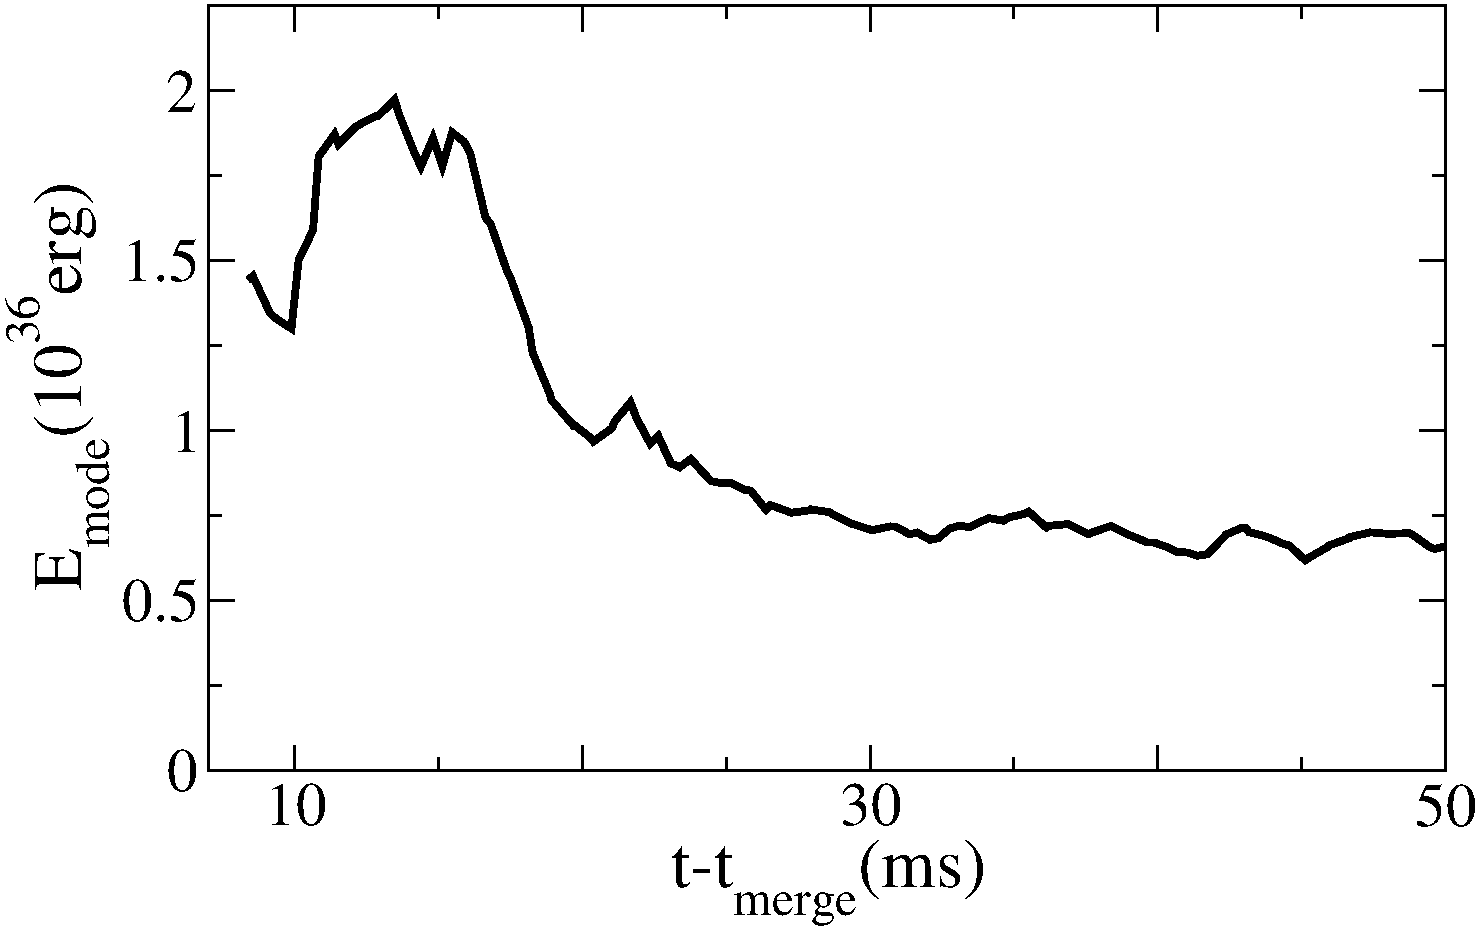
\includegraphics[width=9cm]{Figures/ModeEnergy}
\caption[Disk equilibrium over time]{The deviation of the accretion disk from
equilibrium, as measured by the difference between the
actual and equilibrium orbital energy.}
\label{fig:mode}
\end{figure}

\begin{figure}
\centering
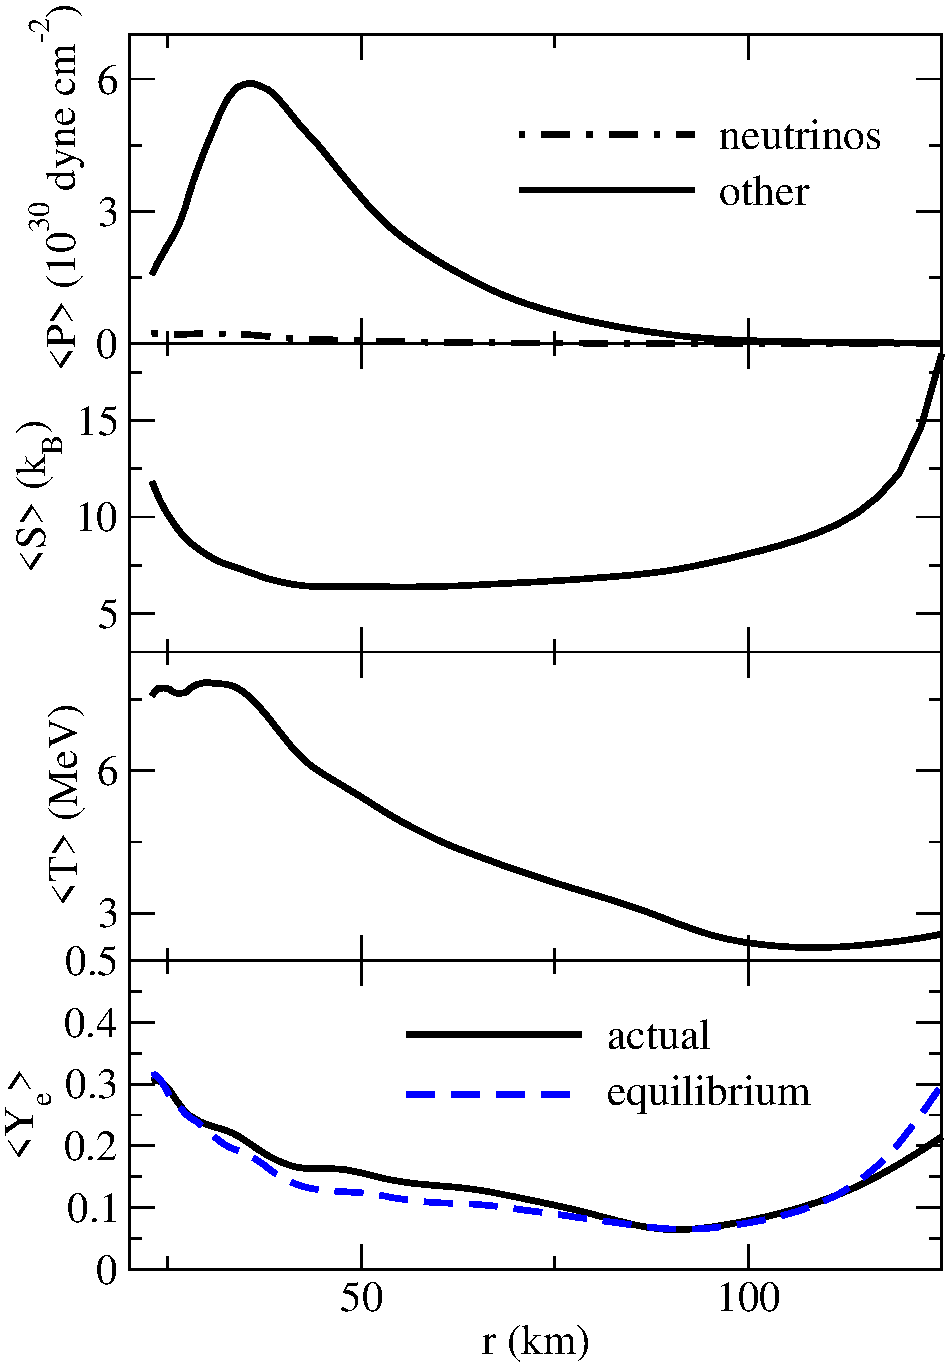
\includegraphics[width=9cm]{Figures/profiles}
\caption[Radial profiles of disk thermodynamics]{
Profiles of the azimuthally- and vertically-averaged pressure, entropy, temperature, and
electron fraction 40~ms after merger. For the pressure, we plot separately
the contributions from the neutrinos and everything else (nucleons,
electrons, photons).  For $\langle Y_e \rangle$, we show both the actual value and the
equilibrium value (at which $R_{\nu}=R_{\nu_e}-R_{\overline{\nu}_e}=0$ for the
given density and temperature profile).
}
\label{fig:profiles}
\end{figure}

\subsubsection{Disk Stability}

In Fig.~\ref{fig:profiles}, we plot the density-averaged pressure $P$,
entropy $S$, temperature $T$, and electron fraction $Y_e$ as functions
of circumferential radius---reducing from three dimensions by averaging
these functions vertically and azimuthally.
The entropy profile is fairly flat in
the bulk of the disk, with the exception of a steep negative gradient
($dS/dr<0$) 
in the hot inner region.  Since in this region pressure increases with
radius, this entropy gradient is actually a stabilizing force.  The $Y_e$
gradient also affects the
buoyancy,
but for these profiles,
its effect is much smaller than that of the entropy.  The relativistic
Solberg-H{\o}iland critera for convective stability of an axisymmetric
equilibrium fluid are given, for a coordinate basis in which
$\psi_{tr}=\psi_{r\phi}=0$, by \citep{segu1975-rot_stability}
\begin{eqnarray}
\label{SH1}
\vec{\gamma}\cdot\vec{\nabla} L + (\rho h)^{-2}(\partial\mathcal{U}/\partial S)_P
\vec{\nabla} P\cdot\vec{\nabla} S &\ge& 0\ , \\
\label{SH2}
(\partial\mathcal{U}/\partial S)_P(\vec{\gamma}\times\vec{\nabla}P)\cdot
(\vec{\nabla}S\times\vec{\nabla}L) &\ge& 0\ ,
%r^{-3}\nabla_rL^2 - (c_p\rho)^{-1}\nabla P\cdot\nabla S &>& 0 \\
%\nabla_zP(\nabla_rL^2\nabla_zS - \nabla_zL^2\nabla_rS) &<& 0, 
\end{eqnarray}
where $\mathcal{U}=\rho+\rho\epsilon$ is the total energy density and
\begin{equation}
\vec{\gamma} = (u^0u_0)^2[(1-v^2)(\psi_{\phi\phi})^{-1}u_0{}^2\vec{\nabla}L
-\vec{\nabla}\Omega]\ .
\end{equation}
Equations \ref{SH1} and \ref{SH2} correspond to the familiar Newtonian
radial and vertical stability conditions, respectively. 
The first term in Eq.~\ref{SH1} dominates everywhere inside
of $r\approx 120$\,km, so $dL/dr$ determines the stability to radial convection
through most of the disk. 
The condition for stability is met except in the inner edge ($r<27$\,km)
of the disk.  This inner region should be unstable.  The unstable
gradient persists, and it is presumably connected to the inability
of the inner disk to settle to stationary axisymmetry.  The outer
disk also has an unstable angular momentum gradient ($dL/dr<0$), but
it is stabilized by a strong positive entropy gradient. 
The entropy does not change much with height, but we do
identify a negative gradient in a region near the equator, leading to
an instability according to Eq.~\ref{SH2} there.  Buoyant forces would be
expected
to correct this gradient on timescales $(-N_{\rm BV,z}^2)^{-1/2}\sim 10$ms, but
apparently other processes (see Section~\ref{sec:neutrinodisk} on processes
that affect entropy
evolution) are sufficient to keep the entropy profile roughly fixed.

In addition to local instability, the disk could be susceptible to global
instabilities involving amplification of the unstable mode across its corotation
radius, located at $r \approx 27\rm\,km$, given the mode's pattern
speed (e.g \citealt{papa1985-rot_stability}).

The temperature is high ($\sym 8$~MeV) in the inner disk, and in these
regions, the contribution of trapped neutrinos to the total pressure is as
high as 12\%.  In the bulk of the disk, the neutrino pressure is
negligible.

\subsection{Neutrino-Driven Disk Evolution}
\label{sec:neutrinodisk}

\subsubsection{Disk Neutrino Luminosity}

\begin{figure}
\centering
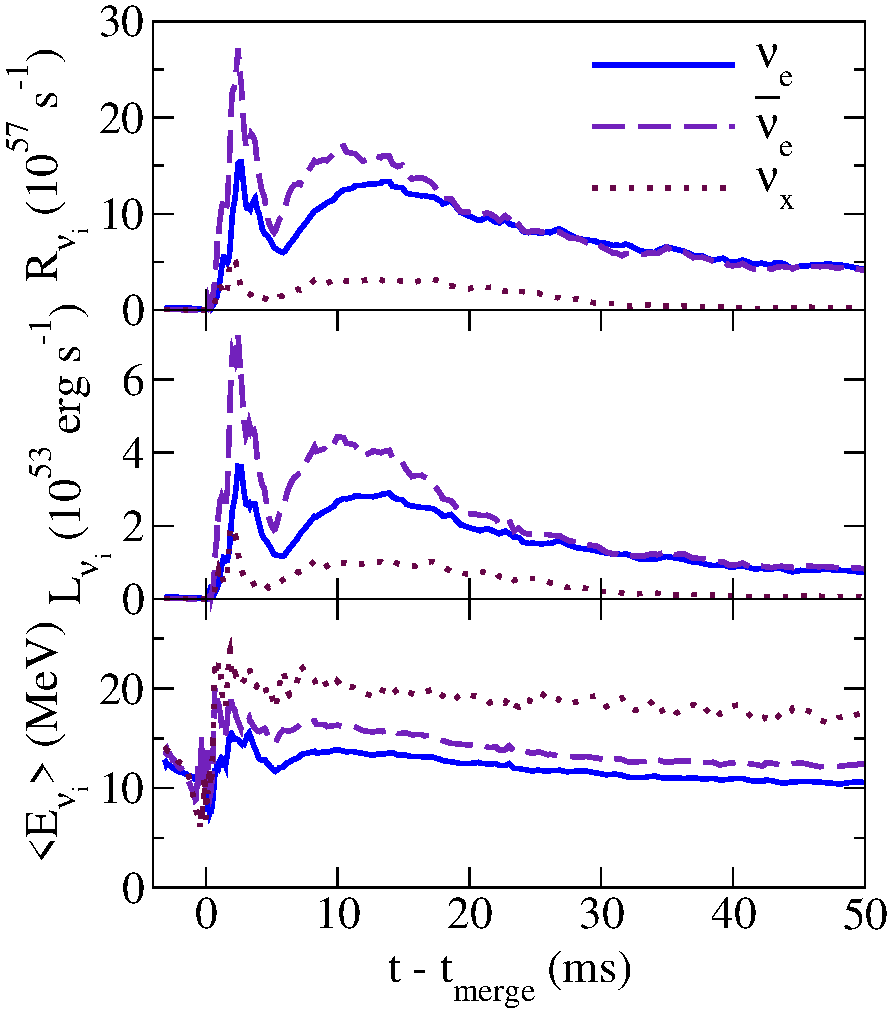
\includegraphics[width=11cm]{Figures/neutrinos_by_species}
\caption[Neutrino emission characteristics by species]{
Neutrino emission characteristics by species.
{\em Top panel}: lepton number luminosity, $R_{\nu_i}$
(in units of $10^{57}\rm\,s^{-1}$).
{\em Middle panel}: energy luminosity, $L_{\nu_i}$
(in units of $10^{53}\rm\,erg\,s^{-1}$).
The total luminosity is given by $L_{\nu_e}+L_{\bar{\nu_e}}+4L_{\nu_x}$. 
$L_{\nu_x}$ is, thus, the luminosity of each individual $\mu$ and $\tau$
species.
{\em Bottom panel}: average neutrino energy $\langle \varepsilon_{\nu_i} \rangle$
(in units of MeV).
All plots are taken from the L3 simulation, and are calculated for
an observer at $r \rightarrow \infty$.
}
\label{fig:neutrinos_by_species}
\end{figure}

Fig.~\ref{fig:neutrinos_by_species} breaks down the energy and number
emission by neutrino species.  Initially, $\overline{\nu}_e$
dominates over $\nu_e$ emission, as would be expected for a neutron-rich,
proton-poor gas.  As emission continues, protons become more numerous, and
the neutrinosphere cools, so that positrons become less common than electrons. 
(The electrons are mildly degenerate, $\mu_e/k_BT\approx 1$, so the relative
ratio of electron to positron density is quite sensitive to temperature.)
Thus, $R_{\nu_e}$ and $R_{\overline{\nu}_e}$ become closer.  At 20~ms after merger,
these emission rates are sufficiently balanced that $Y_e$ thereafter
evolves on the slightly longer timescale on
which the disk itself is changing.  In Fig.~\ref{fig:profiles}, we 
compare the actual $Y_e$ to the equilibrium $Y_e$ profile, i.e. to the
distribution $Y_e=Y_e{}^{\rm eq}$ for the given $\rho$ and $T$, that would yield
$R_{\nu}=R_{\nu_e}-R_{\overline{\nu}_e}=0$ everywhere in our leakage scheme. 
At early times,
$Y_e < Y_e{}^{\rm eq}$ for most of the matter and $Y_e$ grows.  At late times
(as in the figure), the inner disk is nearly in equilibrium, but
$Y_e > Y_e{}^{\rm eq}$ in the rest of the disk, so the average $Y_e$ decreases
slowly.  The low-density outer region radiates, and thus responds to emission
imbalances, much more slowly.  It is still in its initial $Y_e$ growth phase.
The average energy per neutrino, given by $L_{\nu_i}/R_{\nu_i}$, averaged in
time over the disk evolution, is about 12, 15, and 19~MeV for
$\nu_e$, $\overline{\nu}_e$, and $\nu_x$ neutrinos respectively;
the average neutrino energies are not constant, but decrease at a rate of 1~MeV per 10~ms.
When one adds together all four species of $\nu_x$ neutrinos, there are still fewer
of them emitted than $\nu_e$ or $\overline{\nu}_e$ neutrinos, but their
average energy is sufficiently higher ($\nu_x$ are emitted from the hotter regions
in the disk interior) that their combined luminosity is slightly larger than
$L_{\nu_e}$ and $L_{\overline{\nu}_e}$. The fact that $L_{\nu_x}$ is roughly a
quarter of $L_{\nu_e}$ may seem surprising, given that the charged-current emissivity
in the luminous part of the disk is two orders of magnitude higher than the thermal
emissivity.  However, charged-current processes also dominate the opacity, so that the
opacity of the brightest part of the disk is smaller for muon and tau neutrinos
($\tau_{\nu_x}\lesssim 1$) than for electron (anti)neutrinos ($\tau_{\nu_e}\sim 2-5$).

\subsubsection{Neutrino Cooling Effects}

From Fig.~\ref{fig:convergence}, we see that the late-time
neutrino luminosity is around $2\times 10^{53}\rm\,erg\,s^{-1}$
and continuing to drop.  During the early disk phase,
$\dot{M} \approx 1\,M_{\odot}\rm\,s^{-1}$, so the
accretion efficiency is $\eta=L_{\nu}/\dot{M}c^2 \approx 0.1$. 
The disk remains very nondegenerate throughout the simulation, with
the thermal component of the internal energy remaining nearly
a constant 85\% of the total internal energy throughout.
The actual values of the thermal and internal energies
decrease at a rate only about half $L_{\nu}$ (see Fig.~\ref{fig:cooling}).
The rate of loss of thermal energy due to flow out of the grid,
comprised at early times primarily of accretion into the black hole
and at late times primarily of disk outflow, is also comparable
to $L_{\nu}$.  Thus, these energy sinks are being countered
by heat sources sufficient to slow the cooling rate by about a
factor of 3.  Two physical sources of heating in parts of the disk are
adiabatic compression (primarily the observed flattening of the disk
toward the equator as it cools) and shock heating, the latter presumably
occuring in the nonlinearly perturbed regions of the disk.  Adiabatic
flattening alone is insufficient, since we observe that the rate of
total entropy decrease is also much lower than the radiative entropy
loss rate.  Shock dissipation is the more plausible heat source, since
losses in spiral mode energy are of the needed magnitude.
A third physical energy source, recombination of nuclei, does not occur
during the phase of evolution simulated;
the composition of the disk remains $>99$\% free nucleons. 
A nonphysical source of heating would be numerical viscosity. 
This can only be distinguished from true shock heating by
comparing heating rates at different resolutions.  We find that
L2 and L3 have very similar thermal histories, while L1
cools 30\% more slowly, largely due to a difference in the outflows,
although effects of stronger numerical energy dissipation might
also contribute.  The average specific
entropy of the disk provides a clearer sense of whether the remaining
matter is heating or cooling.  Its evolution is included in
Fig.~\ref{fig:globalevolution}.  We see that, after the initial
strong shock heating at disk formation, the entropy begins a slow
decrease.  The fact that different resolutions show good agreement
on the entropy evolution reassures us that numerical dissipation
is not dominating the thermal evolution of the disk.

\begin{figure}
\centering
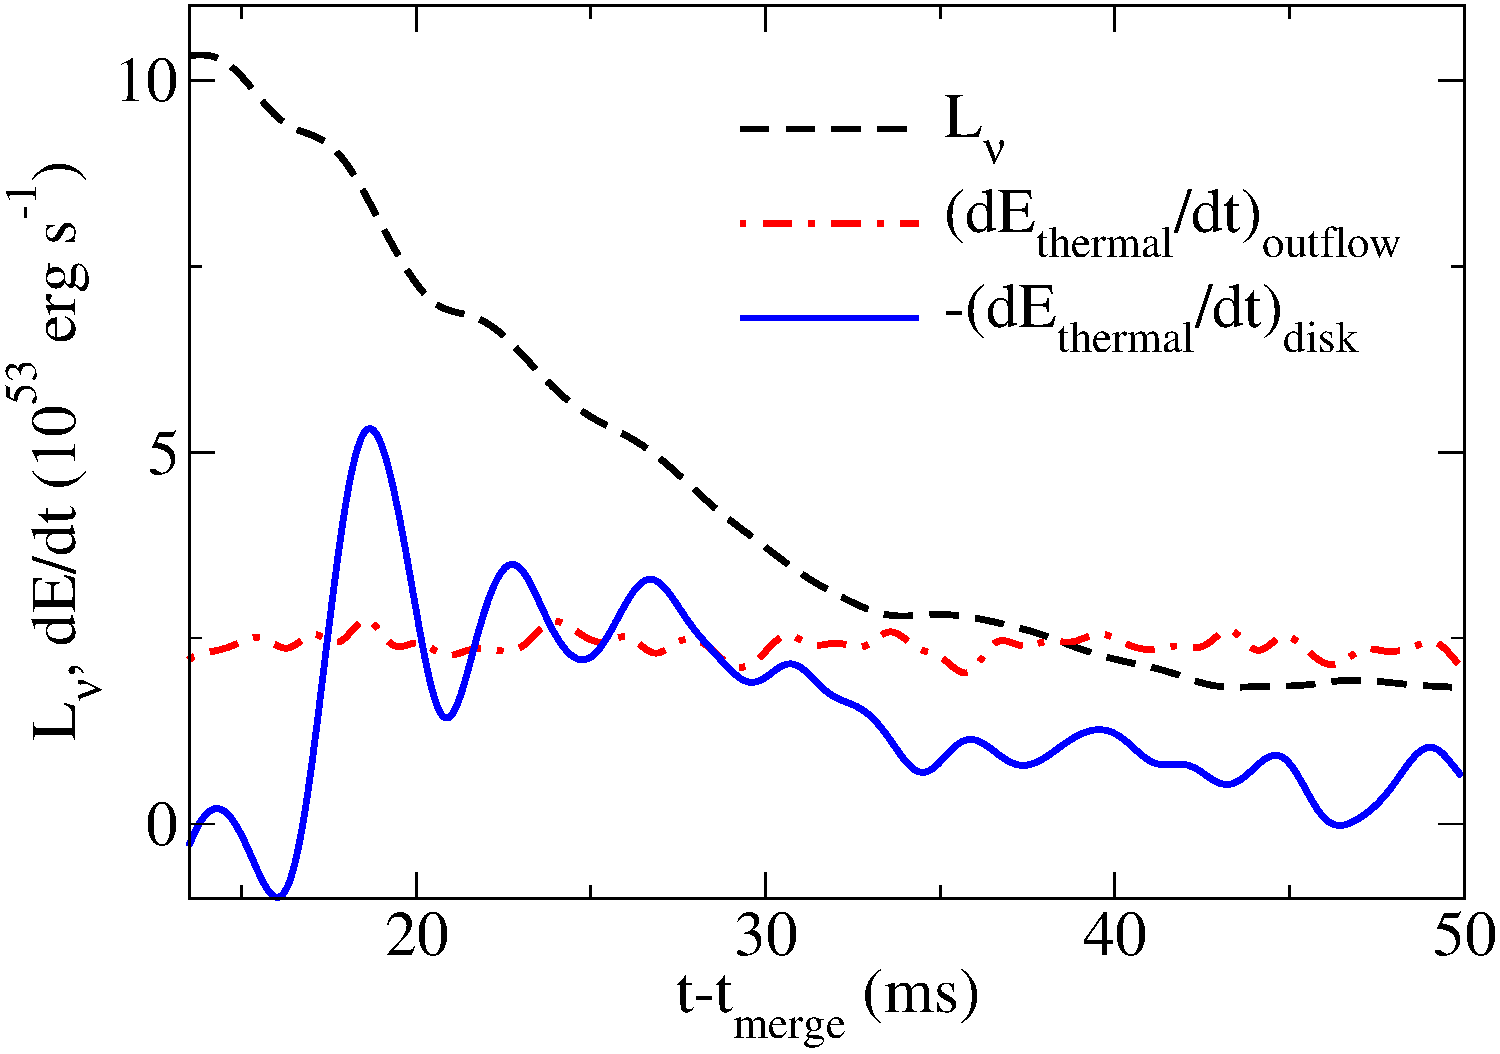
\includegraphics[width=9cm]{Figures/thermal_evolution}
\caption[Analysis of the thermal evolution of the disk]{
The thermal evolution of the disk during its cooling phase. 
$L_{\nu}$ is the neutrino luminosity, $(dE_{\rm thermal}/dt)_{\rm outflow}$
the heat loss due to flows out of the inner and outer boundaries,
and $(dE_{\rm thermal}/dt)_{\rm disk}$ the numerical derivative of the
total thermal energy in the disk.  (The total internal energy
is almost exactly $1.15E_{\rm thermal}$ throughout the Cowling evolution.) 
Numerical derivatives and
outflow measures are noisy, so the curves have been smoothed in
time by convolving with a Gaussian of width 1~ms.
}
\label{fig:cooling}
\end{figure}

\section{Dominant Effect of Neutrinos on Accretion}
\label{sec:comparison}

At least for the very massive, luminous post-merger system studied
here, neutrino cooling and composition changes have a strong effect
on the disk structure, even in the early tens of milliseconds.  We
estimate these effects by comparing simulations carried out with (L1) and
without (L1no$\nu$) the neutrino leakage source terms added to the fluid
equations.

The disk evolved without neutrino cooling develops a significantly
higher, and continually growing, entropy.  This leads to a larger,
more diffuse accretion disk; the maximum density is a factor of ten lower
than for the neutrino-cooled disk, and the density profile lacks the
sharp peak in the inner region seen in Fig.~\ref{fig:thickness}. 
The larger extent of the non-cooled disk causes more matter to escape
through the outer boundary.  During the first 10~ms after merger, the
accretion rate into the black hole for cooled and non-cooled disks is
comparable, and so the L1no$\nu$ disk comes to have a baryonic mass lower by
about 40\% than the L1 disk.  Again, this is a consequence rather than
the cause of the lower density.  At later times, the accretion rate
of the L1no$\nu$ disk drops to very low values, but outflow continues. 

Because of its lower density, the
non-cooled disk actually has a lower average temperature than the
cooled disk (4~MeV vs.\ 5~MeV), despite its higher entropy, during the
first 45~ms after merger.  After this, the temperature of the L1 disk
drops below that of the L1no$\nu$ disk because of neutrino cooling.  As
expected, neutrino emission strongly affects the evolution of $Y_e$. 
For the L1no$\nu$ disk, the electron fraction can only change because of
the accreted or outflowing matter having $Y_e$ that differs from the
average, and this turns out to cause only small changes to the
average (see Fig.~\ref{fig:globalevolution}).

The L1no$\nu$ disk shows the same persistent perturbations from axisymmetry
that are seen in the neutrino-cooled disks.  High-energy, non-equilibrium
flow in the inner disk is still seen.  This confirms that cooling is not
the main driver
of perturbations in the cooled disks.  We find that the geodesic and equilibrium
angular momentum curves show greater deviation for the L1no$\nu$ disk---
the geodesic curves are essentially the same, but $dL/dr$ is about 25\%
shallower for the equilibrium curve in the bulk of the non-cooled disk---
indicating that pressure support makes a stronger contribution to the
equilibrium of this disk.  The entropy profiles have the same general
shape, and the expected stability properties are similar.


% Ray Tracing
\chapter{Properties of Neutrino Emission}
\label{chap:ray_tracing}

The leakage approximation used in Chap.~\ref{chap:leakage} gives us a beginning
understanding of the cooling effects of neutrinos on the accretion disk, or
how the disk changes as it radiates. Through that approximation we have been able
to estimate changes in the energy and composition of the fluid at the position
$x^\alpha$ due to the emission of neutrinos at $x^\alpha$.

However, the leakage approximation teaches us very little about the properties of
that emission. We \emph{can} extract some rough global measures:
1) the sum of the energy losses from all positions in the disk (i.e.\
the volume integral of $Q_{\nu_i}$ defined in Sec.~\ref{sec:leakage})
gives us the total energy luminosity, $L_{\nu_i}$, at any epoch,
2) likewise the sum of $R_{\nu_i}$ gives us the total lepton number luminosity
(also denoted $R_{\nu_i}$),
3) and the ratio of these two luminosities gives us the average neutrino energy,
$\langle \varepsilon_{\nu_i} \rangle$. These three calculations are presented in
Fig.~\ref{fig:neutrinos_by_species}.

But to answer some of the questions presented in Chap.~\ref{chap:overview}, we
need to know more about the radiation field outside of the disk, particularly
how it varies with position, $x^\alpha$, and how it is distributed in energy and
angle, $p_k$.
That is, we need to develop an estimate of the neutrino distribution function,
$f_{\nu_i}(x^\alpha;p_k)$.

Where the mean free path of the neutrinos is long with respect to local fluid
\todo{show this is the case}
scales at $x^\alpha$, $f_\nu(x^\alpha)$ is dependent upon the state of matter
far away from $x^\alpha$. In lieue of solving the Boltzmann equation in full
\todo{ref eqn in Chap.~\ref{chap:intro}}
(which would involve an evolution of a scalar field like those presented in
Chap.~\ref{chap:leakage} for fluid and metric fields, but over a 6-dimensional
phase space manifold with coordinates $\{x^j,p_k\}$, and therefore
computationally out of reach today),
we can capture this nonlocality with a ray tracing solution.
In ray tracing, $f_\nu(x^\alpha;p_k)$ is computed by tracing a neutrino trajectory
backwards from $x^\alpha$ with a momentum $p_k$, keeping track of additions
and depletions to the neutrino number density along that trajectory.
Each ray yields an approximate solution to the Boltzmann equation at a
single point on the phase space manifold of interest. A ray
tracing solution to the Boltzmann equation places an observer at $x^\alpha$,
points him in the direction $p_k$, and asks ``how many neutrinos from that
direction?''
This approximation neglects additions to the neutrino number density due to
scattering into the line of sight (the kind of scattering that gives to the
moon or a streetlamp a halo on a foggy night).
\todo{ref later discussion}

In this chapter I present a ray tracing algorithm for estimating
$f_{\nu_i}(x^\alpha;p_k)$ in relativistic numerical spacetimes and fluid
distributions, I calculate $f_{\nu_i}$ describing neutrino
emission from the model accretion disk from Chap.~\ref{chap:leakage},
and I use these $f_\nu$s to estimate $q_{\nu\bar{\nu}}$, the heating due to
neutrino-antineutrino annihilation in the funnel of the disk.
Because of large uncertainties,
this last calculation should be considered a proof-of-concept for future
calculations. It may also be considered a back-of-the-envelope answer to
the question, ``Can a neutron star--black hole merger drive a gamma ray burst
jet by neutrino processes alone?''

Sec.~\ref{sec:f_algorithm} gives a technical overview of the ray tracing
algorithm and two code tests. Sec.~\ref{sec:f_this_case} presents the distribution
function of the three 'leakage' neutrino species around this model accretion
disk. Secs.~\ref{sec:q_algorithm}~and~\ref{sec:q_this_case} describe the
algorithm for and results from a neutrino-antineutrino annihilation heating
calculation for this model.

\section{Calculating $f_\nu$}
\label{sec:f_algorithm}

In the most comprehensive treatment, a ray tracing solution for $f_\nu$ is calculated
by solving the rendering equation backwards along a trajectory terminating at
$x^a$ with momentum $p_k$:
\todo{derive rendering eqn, or check/ref below}
\begin{equation}
  \label{eqn:rendering}
  f(x^\alpha;p_k) = \int_{x^a}^{\rm far\,away} \diff \lambda \, \mathcal{E}(p_k)
  \exp\left(-\int_{x^a}^\lambda  \diff \lambda' \, \mathcal{A}(p_k)\right)
\end{equation}
where $\mathcal{E}$ and $\mathcal{A}$ are the invariant emissivity and opacity
defined in Chap.~\ref{chap:intro}.
\todo{ref eqns}
For isotropic scattering, $p_k$ only enters $\mathcal{E}$ and $\mathcal{A}$ in the
form $-p_\beta u^\beta$, the neutrino energy in the rest frame of the fluid.
Furthermore, $p_\beta$ may be calculated from $p_i$ by invoking the neutrino mass,
$-m_{\nu_i}^2=p_\beta p^\beta$.
All the neutrino masses are vanishingly small in the case of nuclear
accretion disks, with fluid energy scales of a few MeV. So in the following we
set $m_{\nu_i}=0$.

As $f_\nu$ accumulates along the ray, the integrand in Eqn.~\ref{eqn:rendering}
gets attenuated by the exponential term, which is the optical depth defined in
Chap.~\ref{chap:intro}.
\todo{ref eqn}
At large optical depths, the integrand vanishes exponentially, because fluid
properties on the far side of opaque matter cannot affect the neutrino
distribution function on this side. The exponential behavior of the integrand
leads us to pose a further approximation, that all neutrinos are emitted from
a single point along the trajectory, the neutrinosurface.

In this treatment, the ray is traced backwards until the optical depth becomes
large ($\tau\sim1$). This defines the neutrinosurface at $x_0^\alpha$. The
neutrinos are assumed to decouple from the matter at this surface, and so f
is simply the Fermi-Dirac distribution:
\begin{equation}
  \label{eqn:f_fermi_dirac}
  f(x^\alpha;p_k) =
  \left(\exp\left(\frac{-p_\beta u^\beta(x_0^\alpha)}{T(x_0^\alpha)}
  -\eta(x_0^\alpha) \right)+1\right)^{-1}
\end{equation}
where $T(x_0^\alpha)$ is the fluid temperature at the neutrinosurface, and
$\eta(x_0^\alpha)$ is the neutrino chemical potential scaled by $T$.
We use $\eta$ estimated by the leakage scheme (Eqn.~\ref{mu_nu}).
\todo{other choices for $\eta$}

Because neutrino scattering processes scale with
$\varepsilon^2=(-p_{\nu}^\beta u^\beta)^2$,
\todo{ref intro}
we use the energy-factored opacity $\zeta=\chi/\varepsilon^2$, where $\chi$ is
the cumulative opacity:
\begin{equation}
  \chi = \sum\limits_{{\rm processes}\, i} \chi_i.
\end{equation}
We consider scattering by nucleons and nuclei and absorption onto nucleons,
as described in Sec.~\ref{sec:leakage}.
Because the fluid and spacetime configuration at this late time is approximately
axisymmetric and stationary on the timescale of a neutrino-crossing time
($\sym1$~ms), we trace our geodesics through a single time slice of data,
rather than taking timesteps backwards through previous data slices,
interpolating in between slices. This greatly reduces the memory demands (each
time slice comprises $\sym$1~GB of data) and complexity of the calculation.
\todo{estimate disk changes over 1~ms: from response to leakage referee}

\subsection{Geodesic and Opacity Equations}
\label{ssec:geodesic}
In a general spacetime like that of our disk model, neutrinos do not follow
straight Euclidean paths, but curves that obey the geodesic equation,
\begin{equation}
  \label{eqn:geodesic}
  0=\frac{d^2x^\alpha}{d\lambda^2} + \Gamma^\beta_{\alpha\gamma}
  \frac{dx^\alpha}{d\lambda}\frac{dx^\gamma}{d\lambda},
\end{equation}
This second-order equation may be split into two coupled first-order equations
by choosing the affine parameterization $\lambda$ such that
$dx^\alpha/d\lambda=p^\alpha$ and
$dp^\beta/d\lambda=\Gamma^\beta_{\alpha\gamma}p^\alpha p^\gamma$.
\todo{umm, check p eqn}
The connection coefficients may be calculated from derivatives of the metric,
\begin{eqnarray}
  \label{eqn:christoffel}
  \Gamma^\beta_{\alpha\gamma}
  &=& \psi^{\beta\mu}\Gamma_{\mu\alpha\gamma} \nonumber \\
  &=& \frac{1}{2} \psi^{\beta\mu}
  (\psi_{\mu\alpha,\gamma} + \psi_{\mu\gamma,\alpha} - \psi_{\alpha\gamma,\mu}).
\end{eqnarray}

Neutrinos have rest masses less than a few eV \citep{oliv2014-pdg}.
Therefore, at the neutrino energy scale
of this problem (a few MeV, see Fig.~\ref{fig:neutrinos_by_species}), the
geodesics are essentially null.
\todo{say why this matters}

We integrate the geodesic equations parameterized by coordinate time,
using the formulation introduced by \cite{hugh1994-eh_finding}.
The extensive framework to integrate the \citeauthor{hugh1994-eh_finding}\
equations through a numerical spacetime demands efficient handling of
pointwise interpolation of metric fields to arbitrary positions, reading from
disk and reconstructing into memory the metric data dumped from a previous
simulation, and accurate integration of a system of ordinary differential
equations.
All of this was implemented by a graduate student at Cornell, Andy Bohn, in order
to find event horizons and compute gravitational lensing; the latter was
published in \cite{bohn2015-lensing}.
I piggy backed my ray tracing code on top of his general and efficient framework.

In addition to equations for $x^j$ and $p_k$, we integrate $\tau$, the optical
depth along the ray. Thus our entire system of equations is
\begin{eqnarray}
  \label{eqn:geo_x}
  \frac{dx^j}{dt} &=& g^{ji}\frac{p_i}{p^t} - \beta^j \\
  \label{eqn:geo_p}
  \frac{dp_k}{dt} &=& -\alpha \alpha_{,k}p^t + \beta^i_{,k}p_i
  - \frac{1}{2}g^{ji}_{,k} \frac{p_jp_i}{p^t} \\
  \label{eqn:geo_tau}
  \frac{d\tau}{dt} &=& \frac{\varepsilon^3}{p^t} \zeta,
\end{eqnarray}
where $\alpha$ is the lapse, $\beta^j$ the shift, $g^{ij}$ the inverse
induced metric on the spatial slice, and $\varepsilon$ is the neutrino
energy in the frame comoving with the fluid.

A word on $p^t$, used in Eqns.~\ref{eqn:geo_x}--\ref{eqn:geo_tau}.
As is well-known, $p_t$ does not change along a geodesic trajectory if the
spacetime is stationary. (This result may be derived directly from the geodesic
equation, Eqn.~\ref{eqn:geodesic}.)
However, $p^t$, in general, \emph{does} change. We may calculate it in the
following steps: 1) enforce $p_\alpha p^\alpha=0$ by calculating
$p_t=p_i\beta^i-\alpha\sqrt{p_ip_jg^{ij}}$, so that all four components of the
momentum 1-form are known, then 2) calculate the time-component of the dual of
this 1-form, $p^t=\psi^{t\alpha}p_\alpha$, where $\psi^{\alpha\beta}$ may be
computed from the lapse, shift, and induced spatial metric by matrix inversion.

A word on $\varepsilon=-p_\alpha u^\alpha$, used in Eqn.~\ref{eqn:geo_tau}.
In our simulations we don't store $u^\alpha$ directly, but rather the spatial
components of the fluid four-velocity 1-form, $u_i$, and the fluid Lorentz
factor, $W$. (The Lorentz factor doesn't need to be stored, since it may
be calculated from the normalization of $u^\alpha$, by
$W=(u_iu_jg^{ij}+1)^{1/2}$. However it is used throughout our code in enough
places that storing $W$ improves our code's efficiency.)
From these variables, we may calculate
\begin{equation}
  \varepsilon = -p_t W/\alpha -p_i(u_j g^{ij}-\beta^i W/\alpha).
\end{equation}

\subsection{Momentum Conventions}
\label{ssec:p_conventions}
Because of the natural symmetries of our spacetime, it is more convenient to use
momentum components in spherical polar than in cartesian representation. We
describe the map between these representations here.

The neutrino's 4-momentum is fully specified by three numbers, the fourth being
constrained by the mass of the neutrino, which vanishes with respect to the
energies in this problem. Instead of using three of the spherical polar
components, we define a Euclidean magnitude, $p$, and two angles $\alpha$,
$\beta$ which map to the cartesian components of the covariant 4-momentum by
the standard spherical polar map
\begin{align}
  &p_x = p\sin\alpha\cos\beta \\
  &p_y = p\sin\alpha\sin\beta \\
  &p_z = p\cos\alpha,
\end{align}
so that $p = (p_x^2+p_y^2+p_z^2)^{1/2}$.
Fig.~\ref{fig:p_conventions} provides a visual reference for these definitions.

\begin{figure}
  \centering
  \begin{subfigure}{.5\textwidth}
    \centering
    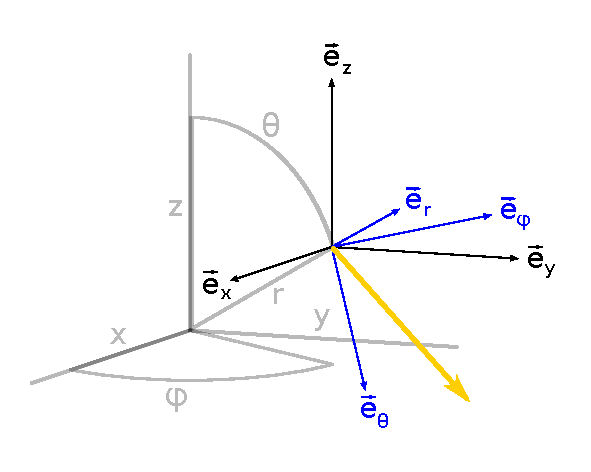
\includegraphics[width=1\linewidth]{Figures/spherical_polar_map}
  \end{subfigure}
  \begin{subfigure}{.45\textwidth}
    \centering
    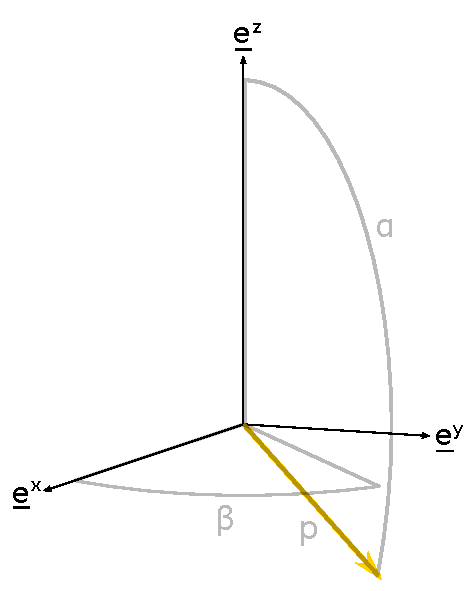
\includegraphics[width=0.8\linewidth]{Figures/neutrino_momentum_conventions}
  \end{subfigure}
  \caption[Conventions for momentum components]{
    In both diagrams, the broad yellow arrow represents the neutrino's momentum.
    \emph{Left Figure}:
    Spatial basis vectors ($\vec{e}_i\equiv\partial/\partial x^i$)
    at a representative position on the manifold.
    The coordinates $\{r,\theta,\phi\}$ are defined with respect to
    $\{x,y,z\}$ by the standard spherical polar to cartesian map
    (e.g.\ $x=r\sin\theta\cos\phi$).
    The spherical basis vectors are blue, and the cartesian basis vectors black.
    \emph{Right Figure}:
    The cotangent space at the neutrino's position.
    The neutrino momentum 1-form, $p_\mu$,
    may be written componentwise using the basis dual to $\vec{e}_i$
    ($\underline{e}^i\equiv dx^i$).
    The neutrino momentum is completely specified by three numbers.
    We use $\{p_t$,$\alpha$,$\beta\}$, which describe the cartesian spatial
    components of $p_\mu$ with the standard spherical polar to cartesian map
    (e.g.\ $p_x=p\sin\alpha\cos\beta$).
    The $p$ in these formulae is the Euclidean magnitude,
    $p = (p_x^2+p_y^2+p_z^2)^{1/2}$, related to $p_t$ by
    Eqns.~\ref{eqn:p_to_pt}~and~\ref{eqn:angular_factor}.
    (Note, we draw the neutrino's momentum vector embedded in the
    spatial manifold in the left figure, even though it properly lives only in
    the cotangent space in the right figure.)
    }
  \label{fig:p_conventions}
\end{figure}

To clean up some future calculations, we also define a 1-form on the
spatial manifold, $\Omega_i$, so that
\begin{align}
  &\Omega_i :\equiv (\sin \alpha \cos \beta, \sin \alpha \sin \beta, \cos \alpha) \\
  &p_i = p\,\Omega_i.
\end{align}

The fourth component of the momentum is constrained by the null condition,
$0=\psi^{\mu\gamma}p_\mu p_\gamma$.
In the 3+1 foliation of spacetime, we have
\begin{equation}
  \psi^{\mu\gamma}p_\mu p_\gamma
  = -\frac{1}{\alpha^2} p_t^2 + \frac{2}{\alpha^2} \beta^i \Omega_i p\, p_t
  + (g^{ij}-\frac{\beta^i \beta^j}{\alpha^2}) \Omega_i \Omega_j p^2, \nonumber
\end{equation}
whose solution is
\begin{equation}
  \label{eqn:p_to_pt}
  p_t = C(\Omega_i) \, p
\end{equation}
\begin{equation}
  \label{eqn:angular_factor}
  C(\Omega_i) \equiv \beta^i \Omega_i \pm
  \alpha \sqrt{g^{ij} \Omega_i \Omega_j}.
\end{equation}

As a check it is easy to confirm that for
$\psi_{\mu \nu}=\eta_{\mu \nu}:=\text{diag}(-1,1,1,1)$,
$C \rightarrow -1$, recovering the flat space connection between time and space
components of momentum. This check also confirms that we use the minus sign in
Eqn.~\ref{eqn:angular_factor}.

In some cases I will break from this convention with a simple rotation, in order
to have a momentum basis oriented with respect to the radial direcion, $\hat{r}$.
I label momentum colatitude and azimuthal angles in the rotated frame as $A$
and $B$ respectively. These angles are related to $\alpha$ and $\beta$ by a
simple Euler rotation, the specifics of which are irrelevant to this thesis.

\subsection{Numerical Integration of the Ray Equations}
\label{ssec:timestepping}
Eqns.~\ref{eqn:geo_x}--\ref{eqn:geo_tau} are solved by discretizing time and
performing a numerical integration.
I describe that process here.

A first-order ordinary differential equation has the form
\begin{equation}
  \partial_t u = L(u),
\end{equation}
which may be discretized into timesteps.
The value of $u$ at the $n$-th timestep is updated to its value
$\Delta t$ later by a fifth-order-accurate Dormand-Prince algorithm,
represented here abstractly as DP5[...]:
\todo{cite?}
\begin{equation}
  u^{n+1} = {\rm DP5}[L,u^n,\Delta t].
\end{equation}

As a high-order integration method, DP5 consists of a series of sub-steps.
Each sub-step evaluates the equation's right hand side, $L(u)$, using $u$ from
the previous step.
\todo{also dense output}
DP5 is an embedded Runge-Kutta algorithm, designed to also yield
a fourth-order-accurate solution with few additional evaluations of $L(u)$.
The difference in $u^{n+1}$ between the fourth- and fifth-order-accurate
solutions gives an estimate of the error for that step size. If this error is
larger than some threshold, we reduce the timestep, and try again from $u^n$.
\todo{Abs-Rel explicit}

The DP5 algorithm works as well for a system of coupled equations,
like the seven components of Eqns.~\ref{eqn:geo_x}--\ref{eqn:geo_tau}:
$\{x^x,x^y,x^z,p_x,p_y,p_z,\tau\}$.
In this case, the above prescription holds, but we think of $u$ as a
vector and $L$ as a vector-valued vector function.

We terminate the ray at the neutrinosurface, where $\tau=1$.
However, because a priori we do not know how much optical depth will accumulate
over a given timestep, we simply overstep the neutrinosurface, terminating at
the step N for which $\tau^{N-1}<1$ and $\tau^N\geq1$. Using the DP5 sub-steps
to interpolate $\tau$ to any time between $t^{N-1}$ and $t^{N}$, we search
this domain for the time $t_0$ that solves the equation
$\tau(t)=1$, using a robust Newton-Raphson root finding algorithm.
\todo{expected convergence order}
We examine the error associated with the uncertainty in the location of the
neutrinosurface in Sec.~\ref{sssc:f_af_sphere}.

\subsection{Code Tests of $f_\nu$}
\label{ssec:f_tests}
To test our code, we compute $f_\nu$ in two scenarios for which the analytic solution
is known.

\subsubsection{Homogeneous Minkowski}
\label{sssc:f_homo_mink}
In a homogeneous medium of temperature $T$, opacity $\zeta$, and neutrino chemical
potential $\eta$, on a flat spacetime manifold, $f_\nu$ is isotropic and homogeneous:
\begin{equation}
  f(x^\alpha;p_k) \rightarrow f(\varepsilon)
  =(e^{\varepsilon/k_{\rm B}T-\eta}+1)^{-1}
\end{equation}
The solution is scale-invariant because the observer sits inside of a
neutrinosurface which emits the same number of neutrinos per angle per energy
whether the surface is near (for high-energy rays) or far (for low-energy rays).

Despite this scale-invariance, we may calculate the length of a ray of energy
$\varepsilon=-p_t=p^t$ from Eqn.~\ref{eqn:geo_tau}:
$\ell \equiv c\Delta t = \Delta \tau/\zeta\varepsilon^2$, in order to test the
opacity integration by ray tracing code.

In our code test, we used volume data:
$T=5$~MeV,
$\zeta_{\nu_i}=\{0.01,0.005,0.001\}$~km$^{-1}$~MeV$^{-2}$, and
$\eta_{\nu_i}=\{0.1,-0.1,0\}$.
We sampled the distribution functions by tracing rays of energy
$\varepsilon=10$~MeV, and found neutrinosurfaces at distances of
$\ell_{\nu_i}=\{2.00,1.00,10.0\}$~km and neutrino number densities of
$f_{\nu_i}=\{0.109,0.130,0.119\}$ for each species respectively,
as expected. These results were exact to double precision because the fields
varied smoothly, and interpolation was exact.

\subsubsection{Hot Compact Star}
\label{sssc:f_af_sphere}
Outside of a hot, compact, non-rotating star in dynamical equilibrium, the
spacetime is spherically symmetric and stationary. The only solution of that
kind satisfying Einstein's equations is the Schwarzschild spacetime.
In Schwarzschild spherical polar coordinates, the metric takes the form
$\psi_{\mu\gamma}(r):={\rm diag}\left(-\alpha^2(r),\alpha^{-2}(r),r^2,r^2\sin^2\theta\right)$,
where the lapse is $\alpha(r)=(1-R_g/r)^{1/2}$, and the gravitating mass is
$M=R_g/2$.
(Note, this scenario was examined semi-analytically by Asano and Fukuyama (2000),
\todo{cite properly}
to estimate the neutrino-antineutrino annihilation power outside of a collapsed
stellar core.)

A neutrino is emitted from the neutrinosphere at $R_\nu$, with energy
$\varepsilon'$ in the fluid rest frame.
%(with $u^\beta:=(-\alpha(R_\nu),0,0,0)$, so that
%$p_{\nu t}=-\alpha(R_\nu)\varepsilon'$),
It will be measured by a stationary observer at $r$
%(for whom $U^\beta:=(-\alpha(r),0,0,0)$),
as having a lower energy
$\varepsilon=\varepsilon' \, \alpha(R_\nu)/\alpha(r)$.
Therefore, for momentum angles in the direction of the neutrinosphere,
$f_\nu(\varepsilon)=\left(\exp(\varepsilon/k_{\rm B}T_{\rm eff}-\eta)+1\right)^{1/2}$,
with an effective temperature $T_{\rm eff}=T \, \alpha(R_\nu)/\alpha(r)$,
where $T$ is the fluid temperature measured in the fluid rest frame.
In terms of the conventional momentum variables $\{p_t,\alpha,\beta\}$
introduced in Sec.~\ref{ssec:p_conventions}, we have
\begin{equation}
  \label{eqn:asano_fukuyama_f}
  f(x^\alpha;p_k) \rightarrow f(r;p_t,A)
  =\left\{
  \begin{matrix}
    (e^{-p_t/k_{\rm B}T\sqrt{(1-R_g/R_\nu)}-\eta}+1)^{-1} & A \leq A_{\rm max}(r) \\
    0                                                            & A > A_{\rm max}(r)
  \end{matrix}
  \right.
\end{equation}
where $A$ is the angle $p_k$ makes with a radial ray, and
$A_{\rm max}$ is the half-angular size of the star as viewed from $r$.
In a flat spacetime it's simple: $\sin A_{\rm max} = R_\nu/r$.
But in the Schwarzschild spacetime, where neutrino trajectories bend around the
star,
\begin{equation}
  \label{eqn:angular_extent}
  \sin A_{\rm max} = \frac{R_\nu}{r} \sqrt{\frac{1-R_g/r}{1-R_g/R_\nu}},
\end{equation}
as derived by Asano-Fukuyama (2000).
\todo{cite properly, and fix, this isn't your angle $A$}

Fig.~\ref{fig:f_hot_ns} shows $f_\nu(p_t=20\,{\rm MeV})$ across all angles for
a patch of sky centered on the emitter. The spacetime and the emitter are
characterized by $T=5$~MeV, $\eta=0.1$, $R_g=2\,M_\odot$, $R_\nu=3\,M_\odot$.
To impose a sharp neutrinosphere at $R_\nu$, we use a step function opacity
with $\zeta=10^6\,{\rm Msun}^{-1}\,{\rm MeV}^{-2}$ inside the star.
This scenario represents an unphysically compact star (in fact, this
neutrinosphere coincides with the radius of circular neutrino orbits), but it
serves its purpose here to stress-test the ray tracing code in strong gravity.
For comparison, in the same figure we also show a ray tracing sampling of $f_\nu$
at the same coordinate viewing position for the same star embedded in flatspace.
Both the angular extent of the stars in Fig.~\ref{fig:f_hot_ns}, and the
intensity of neutrinos emitted by their surfaces at this energy agree
with the analytical predictions given by
Eqns.~\ref{eqn:angular_extent}~and~\ref{eqn:asano_fukuyama_f}.

For this test we use a fixed timestep, $\Delta t = 0.2\,M_\odot$,
because the adaptive timestepper described in Sec.~\ref{ssec:timestepping} is
not very effective with discontinuous fields, like $\zeta$. In physical
fluid configurations, we expect to encounter discontinuities also (though
probably not as extreme), and we may have to used fixed timesteps in those
cases also.

In Fig.~\ref{fig:f_hot_ns}, the Schwarzschild case, the variation in $f_\nu$
across the surface of the star is a spurious artifact of our finite timestep:
the redshift is greater along directions whose rays yield an estimate of the
neutrinosurface at $r<R_\nu$, and lesser for neutrinosurfaces at $r>R_\nu$.
\todo{figure showing this effect}

\begin{figure}
  \centering
  \begin{subfigure}{.8\textwidth}
    \centering
    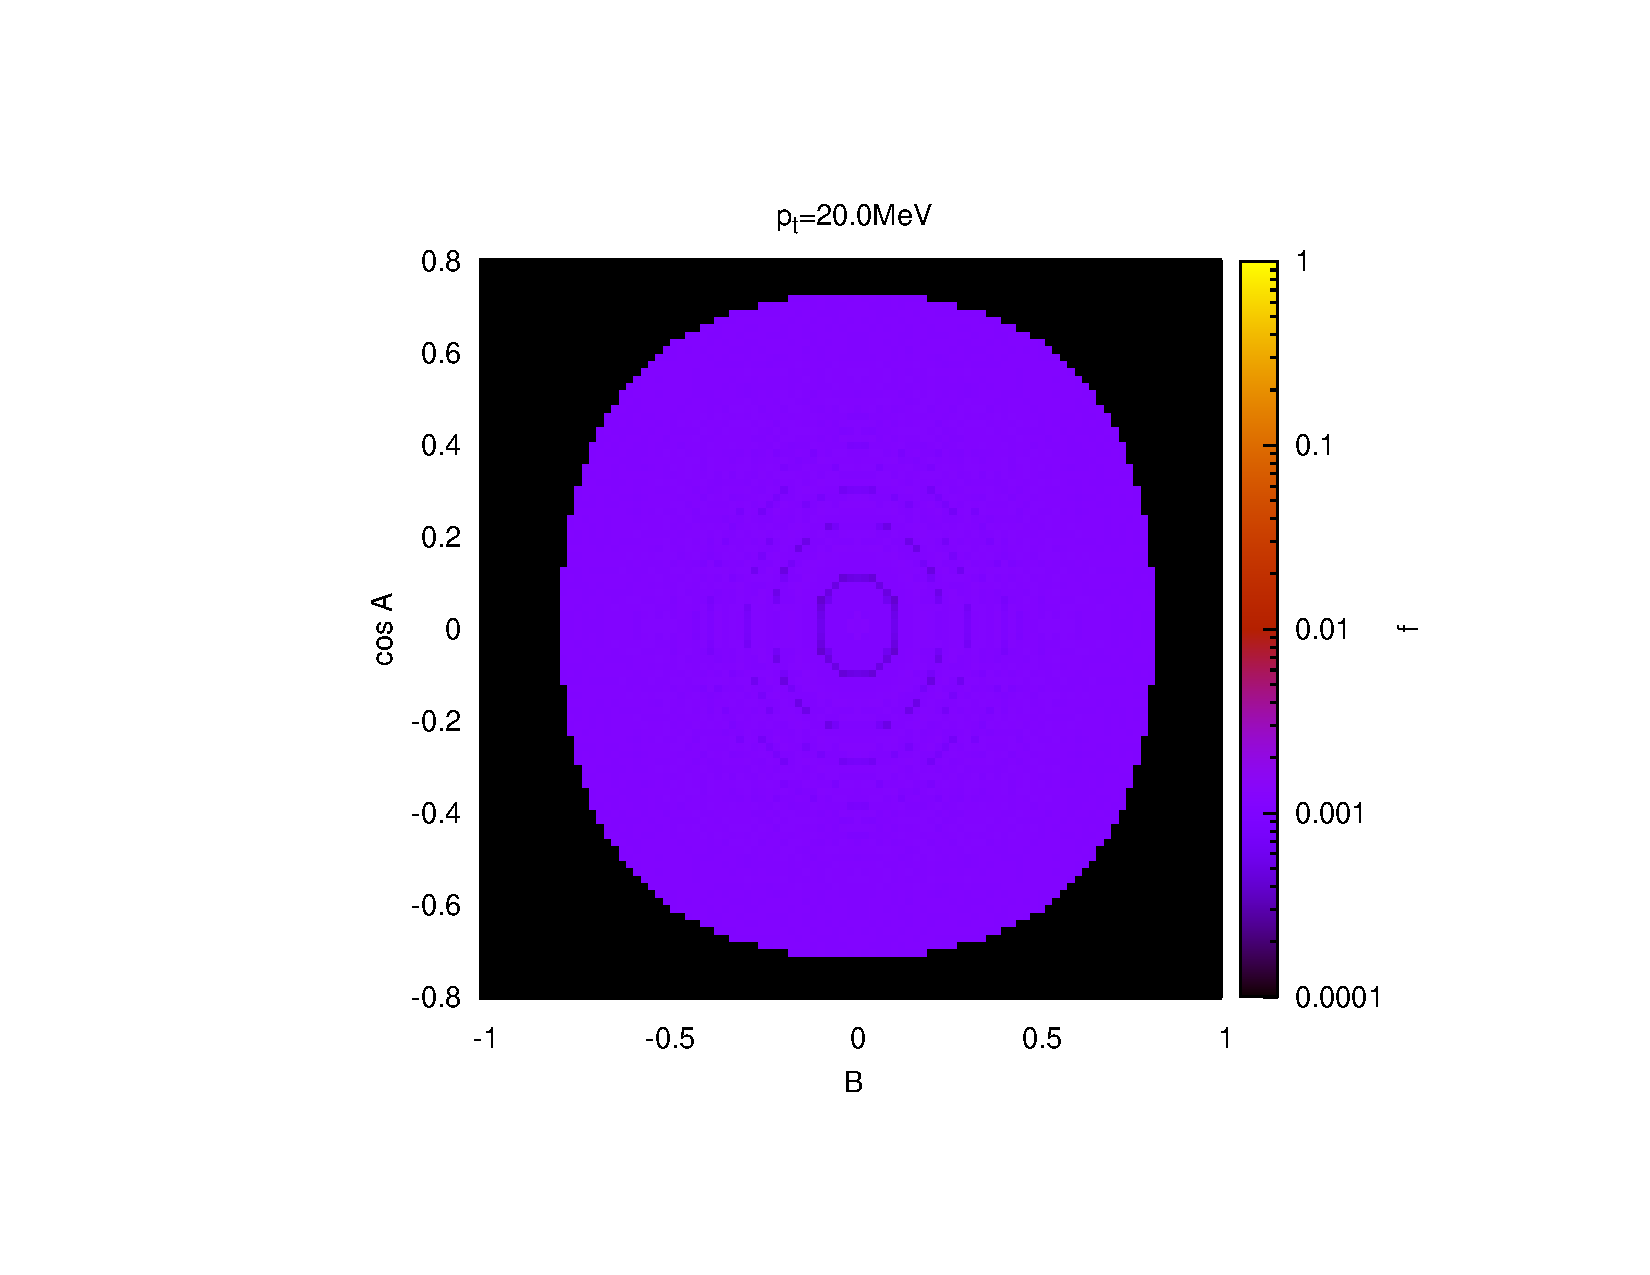
\includegraphics[width=1\linewidth]{Figures/fnue_Alpha_vs_Beta-asano_fukuyama_gr}
  \end{subfigure}
  \begin{subfigure}{.8\textwidth}
    \centering
    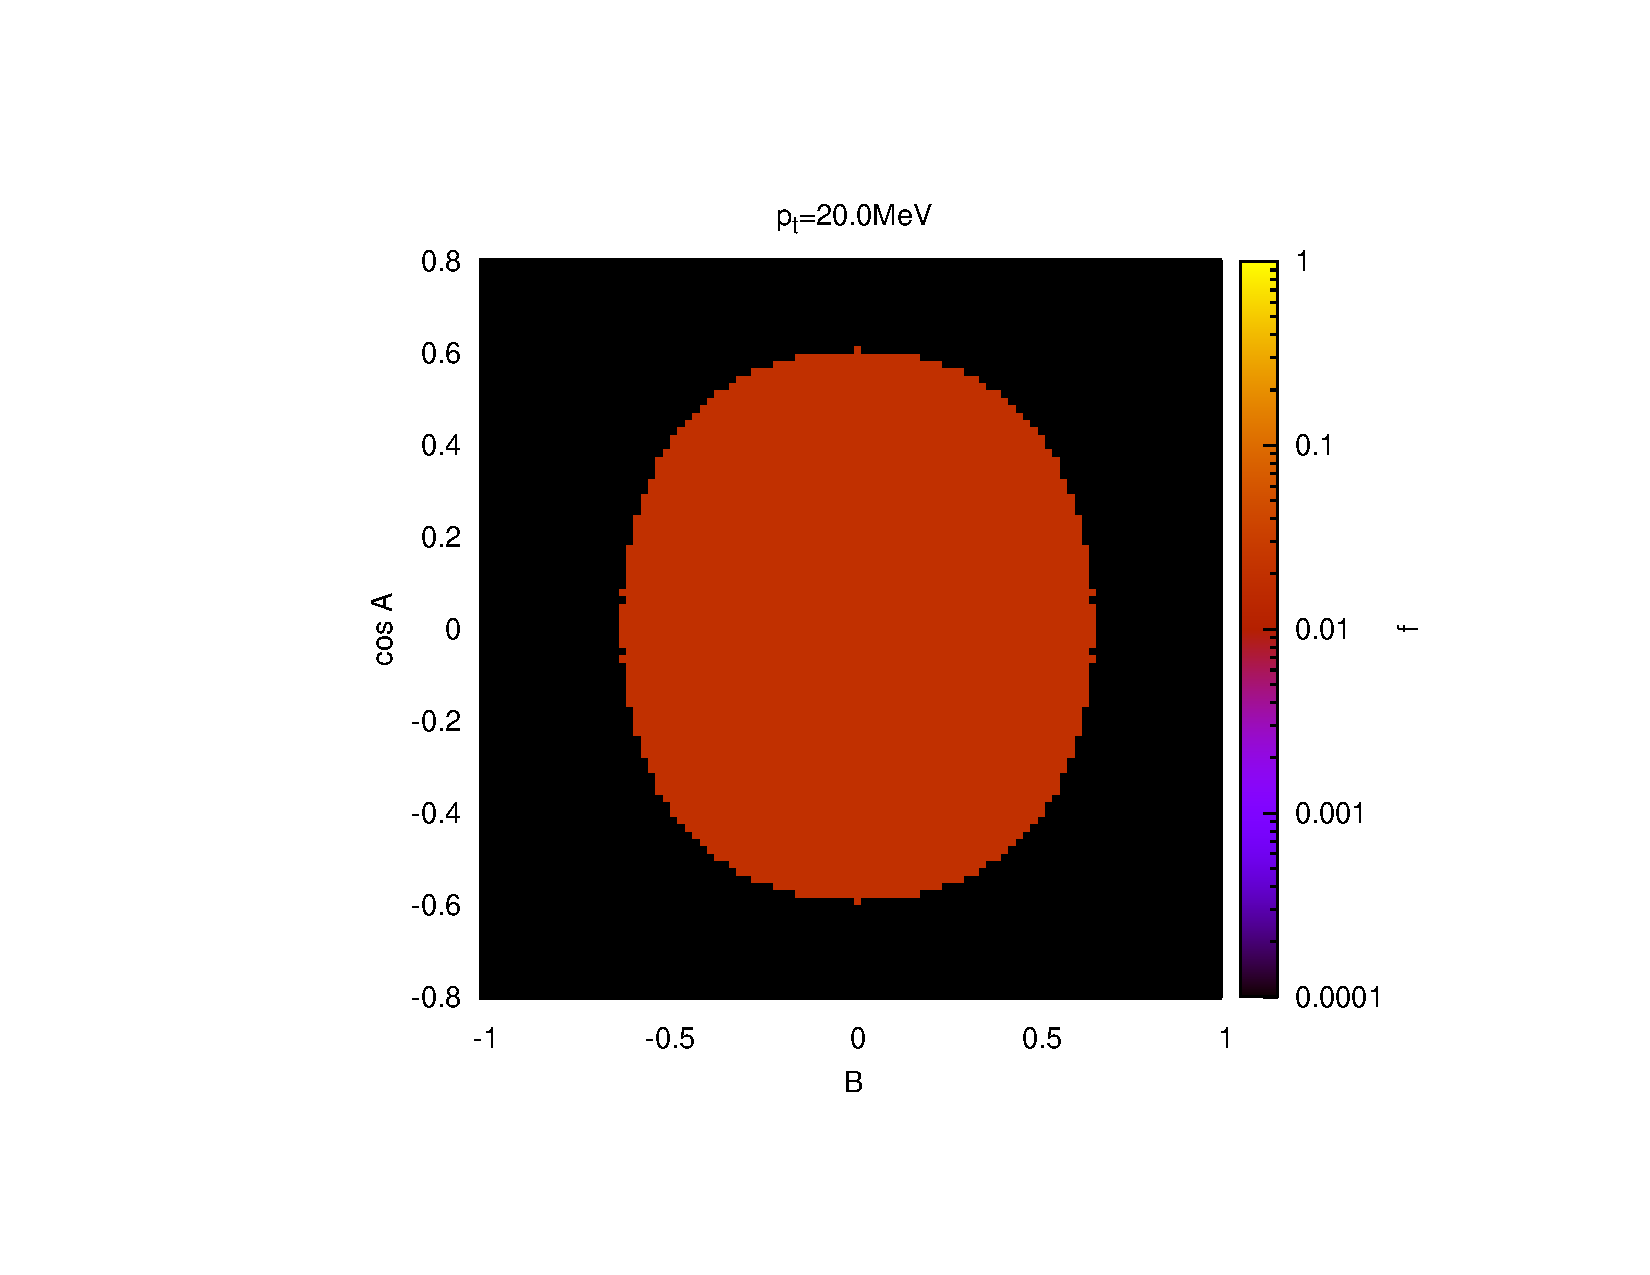
\includegraphics[width=1\linewidth]{Figures/fnue_Alpha_vs_Beta-asano_fukuyama_flat}
  \end{subfigure}
  \caption[$f_\nu$ for a hot compact star: sky map at high energy]{
    $f_\nu$ across a patch of sky in a single energy band, $p_t=20$~MeV.
    The source is a hot compact star: $R_g=2\,M_\odot$, $R_\nu=3\,M_\odot$,
    $T=5$~MeV, and $\eta=0.1$.
    The observer is stationary at Schwarzschild radius $5\,M_\odot$.
    \emph{Top Figure}: Schwarzschild spacetime.
    \emph{Bottom Figure}: Minkowski spacetime.
    These two stars have identical coordinate radii, and identical local fluid
    properties at their neutrinospheres.
  }
  \label{fig:f_hot_ns}
\end{figure}

Fig.~\ref{fig:f_spectrum_hot_ns} presents the energy spectrum emitted by this
surface over the broad band $p_t\in[0.01,100]~MeV$, for both Schwarzschild
and Minkowski cases.
We also show the relative errors in $f_\nu(p_t)$, with respect to the analytic
solution $f_{\nu,\rm ex}(p_t)$. The Minkowski calculation is exact to machine
precision, because location of the neutrinosurface has no effect on $f_\nu$.
But the relative errors in the Schwarzschild case are large, and grow to
20\% at 100~MeV. (It is important to keep in mind that this is not the case
generally, but only when the neutrinosurface is in a steep gravitational
potential.
This will be an important consideration in Sec.~\ref{sec:q_algorithm}:
spectral information at energies near 100~MeV can be important in the
neutrino-antineutrino annihlation calculation because the process depends very
steeply upon the neutrino energies.

\begin{figure}
  \centering
  \begin{subfigure}{.7\textwidth}
    \centering
    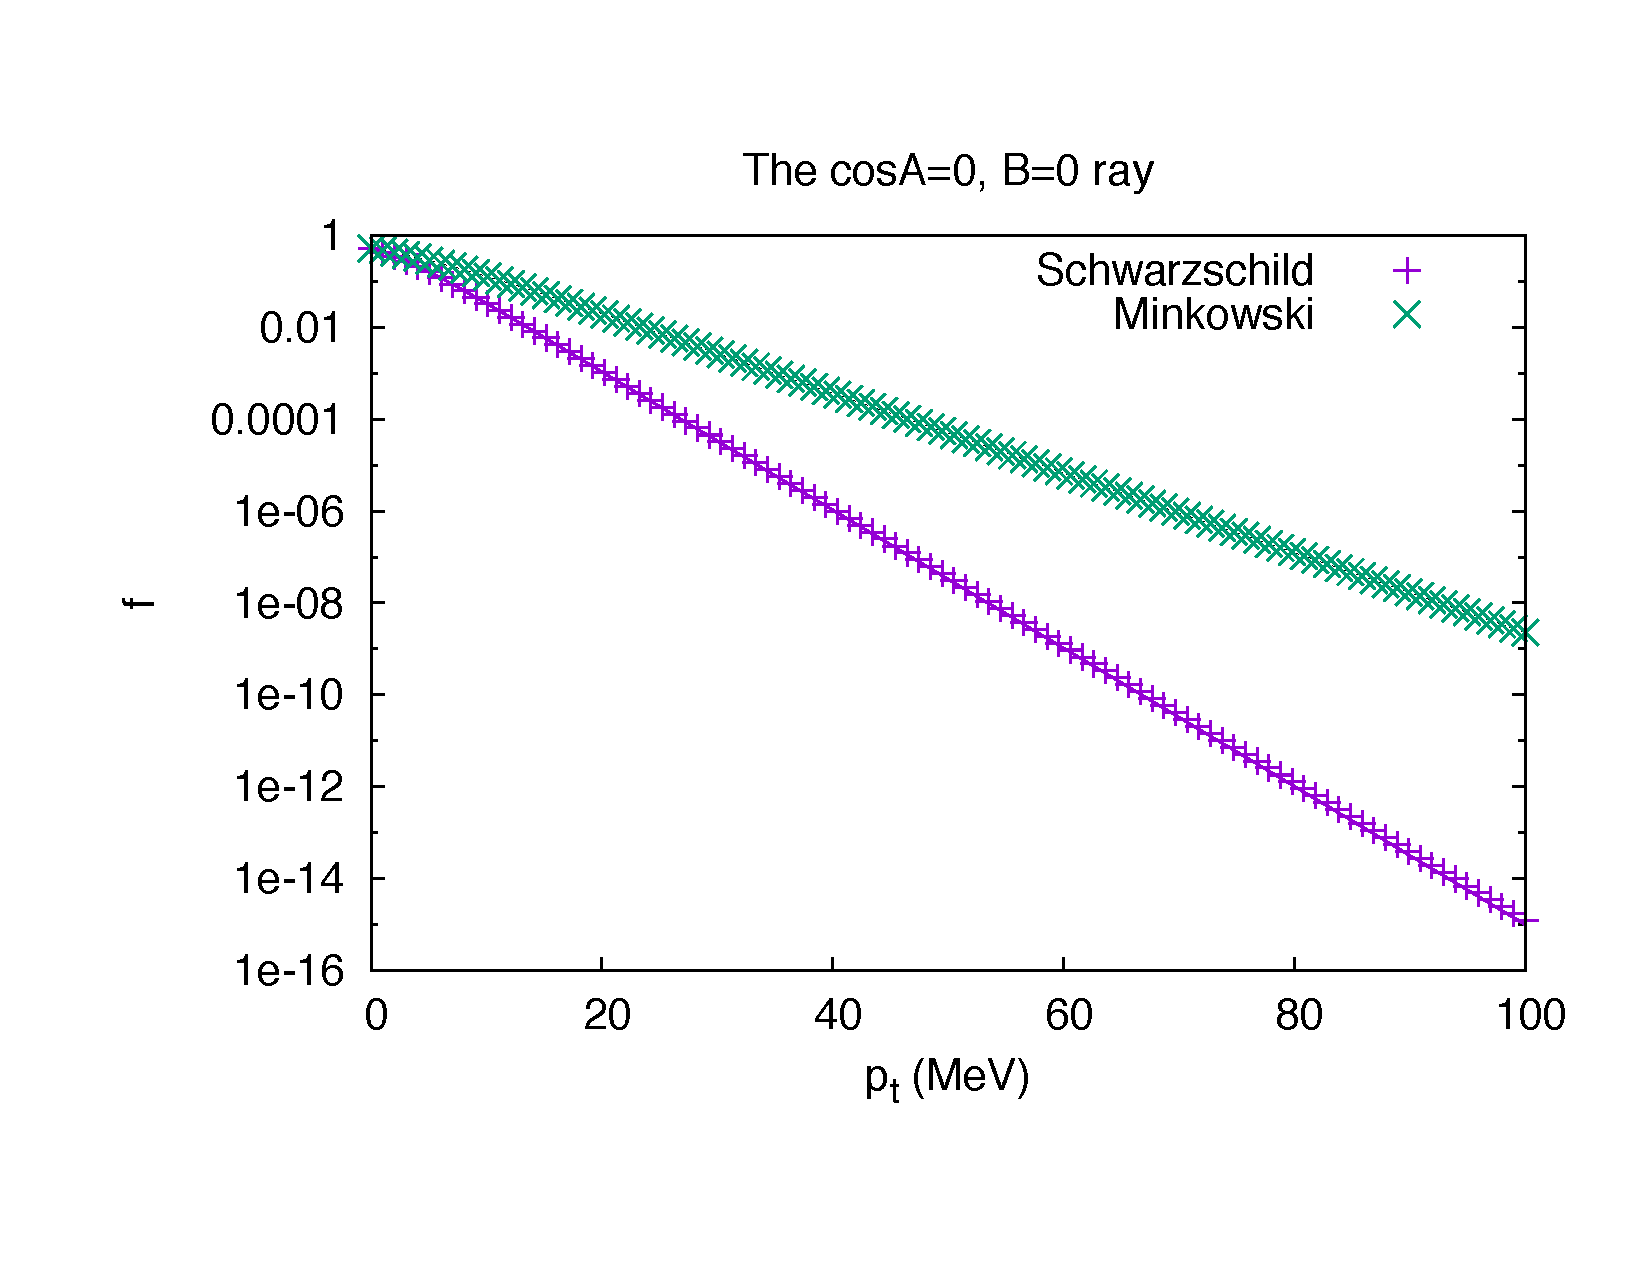
\includegraphics[width=1\linewidth]{Figures/fnue_vs_E-asano_fukuyama}
  \end{subfigure}
  \begin{subfigure}{.7\textwidth}
    \centering
    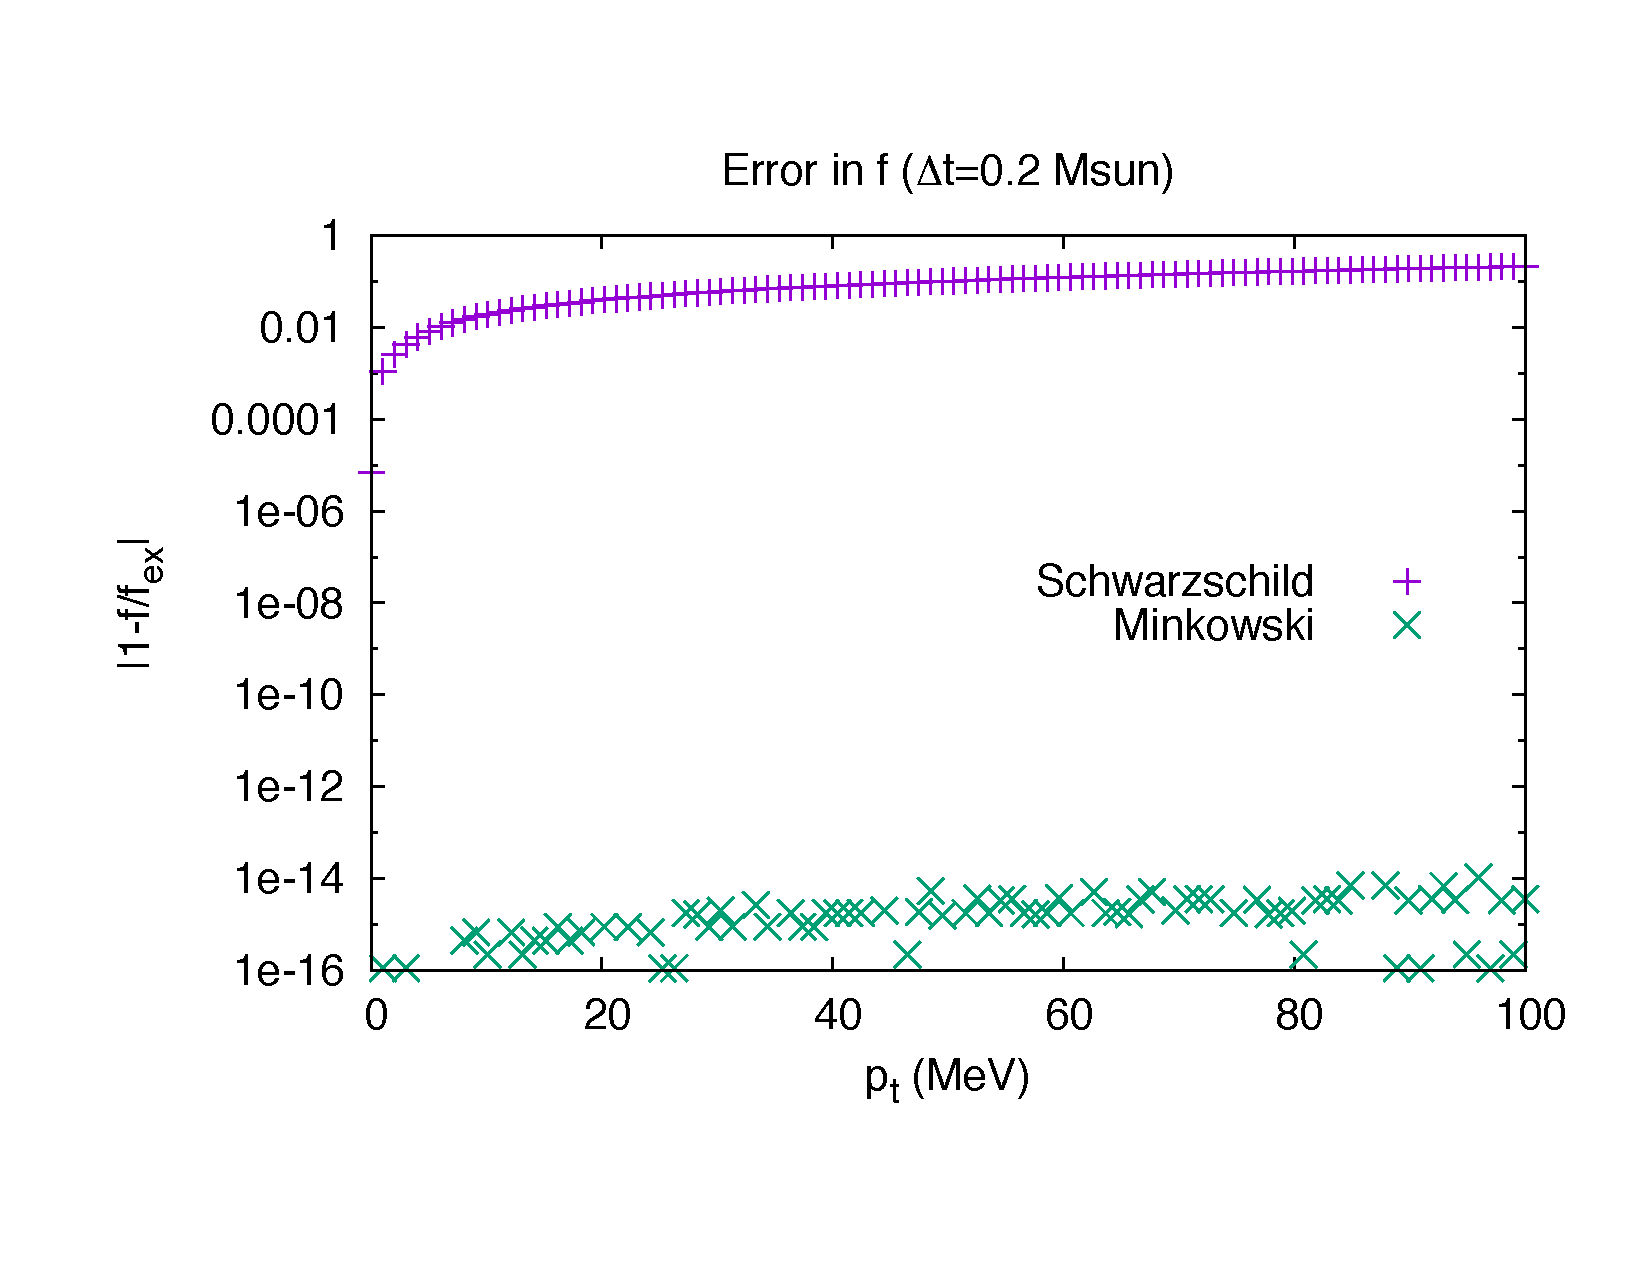
\includegraphics[width=1\linewidth]{Figures/fnueError_vs_E-asano_fukuyama}
  \end{subfigure}
  \caption[$f_\nu$ for a hot compact star: asymptotic energy spectrum]{
    The $p_t$ spectrum of the hot compact star from the same viewing
    position as in Fig.~\ref{fig:f_hot_ns}. These plots show $f_\nu$ sampled by
    the $\cos A=0$, $B=0$ rays.
    \emph{Top Figure}: $f_\nu(p_t)$ in the case of a curved and flat spacetime.
    The exact distribution functions $f_{\nu, \rm ex}(p_t)$ are represented as solid
    lines, which lie directly beneath the data points.
    \emph{Bottom Figure}: The relative error in $f_\nu$ for these two cases.
    For the flat spacetime distribution function, the error bottoms out at
    machine roundoff.
  }
  \label{fig:f_spectrum_hot_ns}
\end{figure}

\section{$f_\nu$ for this Accretion Disk}
\label{sec:f_this_case}

Let us examine the neutrino emission from the post-merger accretion disk model
presented in Chap.~\ref{chap:leakage}. Here we sample $f_\nu$ at two positions,
on the rotation axis and on the equator, about 120~km from the black hole
and at a late time, about 40~ms after merger. At this time the disk has reached
a quasi-equilibrium accretion state, with most of the asymmetry of the merger
having been smeared out by differential rotation, making the model ideal for our
time-independent ray tracing approximation. The disk's luminosity in neutrinos
has decayed to approximately $10^{53}$~erg~s$^{-1}$
(Fig.~\ref{fig:globalevolution}). In this sense, our later calculation of
neutrino-antineutrino annihilation power will provide a lower bound for energy
available to drive a jet.

In fact, 40~ms after a realistic merger with these bulk parameters, we expect
magnetic effects to play a significant role in the accretion dynamics,
\todo{cite someone}
increasing the accretion rate via the magneto-rotational instability, and heating
the disk through a turbulent transport of energy from large scales (bulk kinetic
energy) to small scales (random thermal energy). In this model we neglect this
important physics, and again, in this sense, our later neutrino-antineutrino
annihilation power calculation will provide a lower bound on jet energetics.

\subsubsection{From the Rotation Axis}
\label{sssc:f_this_case_A}

In Figs.~\ref{fig:f_disk_axis_13MeV}~and~\ref{fig:f_disk_axis_34MeV} I display
$f_\nu(\Omega_i)$ over the whole sky, as viewed from the rotation axis, at the
characteristic energies of 13~MeV and 34~MeV. These figures are analagous to
Fig.~\ref{fig:f_hot_ns}. I've sampled $f_\nu$ at these energies because the first is
near the average neutrino energy (see for example
Fig.~\ref{fig:neutrinos_by_species}), and the latter gives us a feel for the
angular distribution of high-energy emission. At lower energies our opaque
disk assumption begins to break down: the disk is transparent to neutrinos at
energies $\lesssim5$~MeV.
\todo{confirm, cite later $\nu\bar{\nu}$ discussion of energy bounds}

All three species of neutrinos represented in the leakage scheme are represented
in these figures: $\nu_e$, $\nu_a \equiv \bar{\nu}_e$, and
$\nu_x \equiv \{\nu_\mu,\bar{\nu}_\mu,\nu_\tau,\bar{\nu}_\tau\}$.

\begin{figure}
  \centering
  \begin{subfigure}{.3\textwidth}
    \centering
    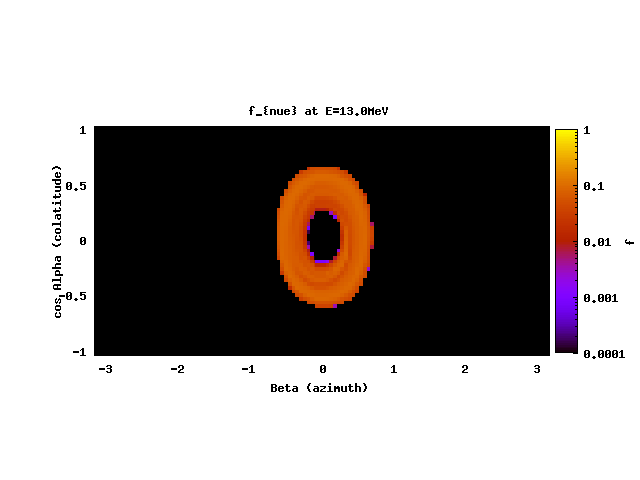
\includegraphics[width=1\linewidth]{Figures/f_nue-A-13MeV}
  \end{subfigure}
  \begin{subfigure}{.3\textwidth}
    \centering
    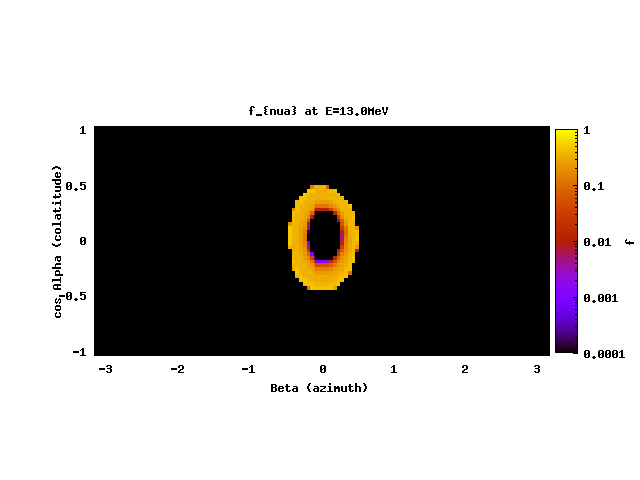
\includegraphics[width=1\linewidth]{Figures/f_nua-A-13MeV}
  \end{subfigure}
  \begin{subfigure}{.3\textwidth}
    \centering
    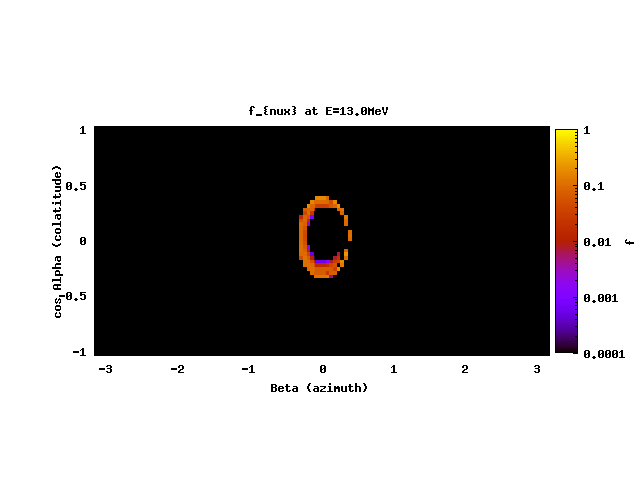
\includegraphics[width=1\linewidth]{Figures/f_nux-A-13MeV}
  \end{subfigure}
  \caption[$f_\nu$ for the disk, from the rotation axis: sky map at average energy]{
    Neutrino distribution functions from the accretion disk over the sky in a
    single energy band, $p_t=13$~MeV. The observer is stationary on the rotation
    axis at coordinate radius 120~km from the black hole. The panels from
    left to right depict $f_{\nu_e}$, $f_{\nu_a}$, $f_{\nu_x}$.
  }
  \label{fig:f_disk_axis_13MeV}
\end{figure}

\begin{figure}
  \centering
  \begin{subfigure}{.3\textwidth}
    \centering
    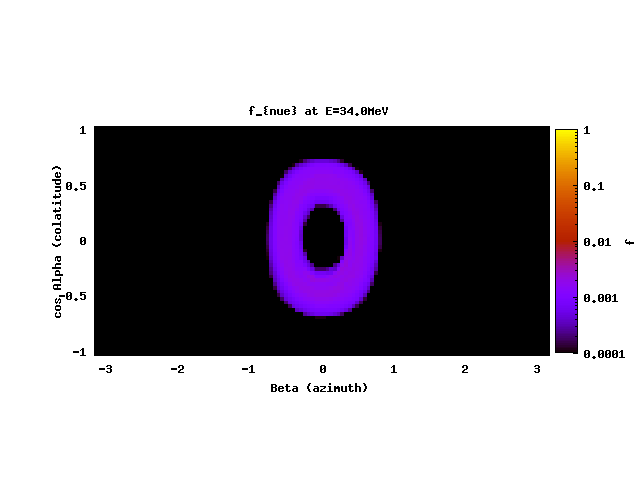
\includegraphics[width=1\linewidth]{Figures/f_nue-A-34MeV}
  \end{subfigure}
  \begin{subfigure}{.3\textwidth}
    \centering
    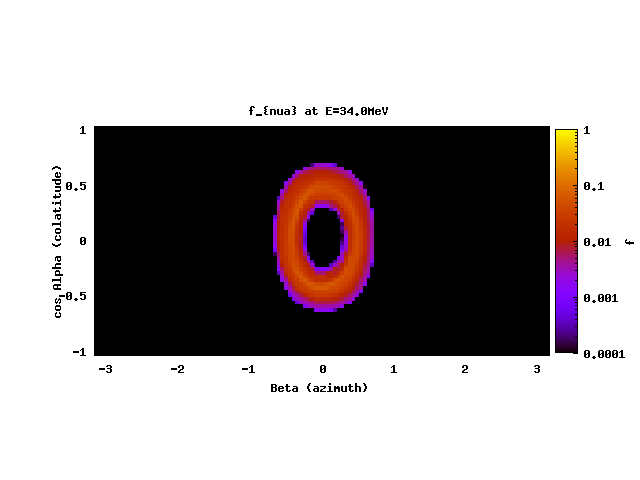
\includegraphics[width=1\linewidth]{Figures/f_nua-A-34MeV}
  \end{subfigure}
  \begin{subfigure}{.3\textwidth}
    \centering
    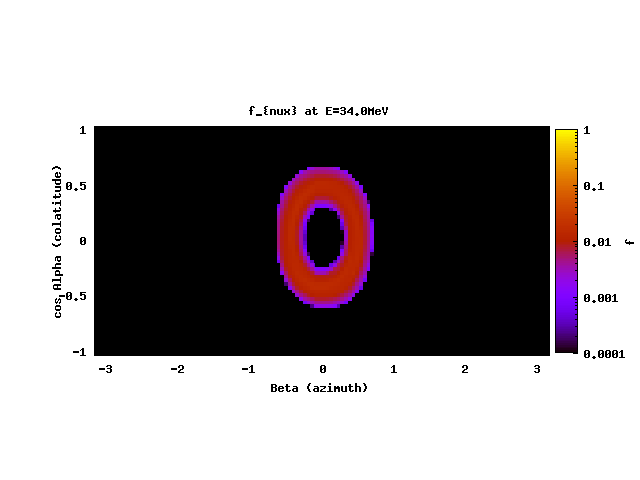
\includegraphics[width=1\linewidth]{Figures/f_nux-A-34MeV}
  \end{subfigure}
  \caption[$f_\nu$ for the disk, from the rotation axis: sky map at high energy]{
    Same as Fig.~\ref{fig:f_disk_axis_13MeV}, but in the energy band $p_t=34$~MeV.
    Left to right, the panels depict $f_{\nu_e}$, $f_{\nu_a}$, and $f_{\nu_x}$.
  }
  \label{fig:f_disk_axis_34MeV}
\end{figure}

Several observations:
\begin{enumerate}
  \item The neutrino surface is larger at higher energy.
    This is because of the opacities' energy dependence,
    $\chi\propto\varepsilon^2$. The higher-energy neutrinosurfaces are further
    away from the black hole, where redshift effects are smaller, than the
    lower-energy neutrinosurfaces. Thus, we may infer that a realistic neutrino
    spectrum is suppressed at low energy compared to that obtained from a
    simple Newtonian calculation.
  \item The brightest ring of emission is not at the extreme inner edge, even
    though the disk temperature is consistently high all the way to the inner
    edge (see for example Fig.~\ref{fig:profiles}). This is a straightforward
    effect of the stronger redshift operating near the black hole.
  \item $f_{\nu_a}$ is brighter than $f_{\nu_e}$
    and emitted from a smaller region.
    \label{item:zeta}
    This is because the disk is less opaque
    to $\bar{\nu}_e$ (see Fig.~\ref{fig:zeta_meridional}). The dominant
    charged-current processes make this clear: in a neutron-rich fluid like that
    of this disk (again see Fig.~\ref{fig:profiles}), $\nu_e$ absorption via
    $\nu_e\,n \rightarrow p\,e^{-}$
    is favored over $\bar{\nu}_e$ absorption via
    $\bar{\nu}_e\,p \rightarrow n\,e^{+}$.
    So the $\bar{\nu}_e$s decouple from the fluid from deeper within the disk,
    at a hotter temperature, and are therefore more luminous.
  \item The $\nu_a$- and $\nu_x$-surfaces are sharp-edged at low energy,
    with little sign of the limb-darkening seen in the $\nu_e$ surfaces.
    \label{item:eta}
    This is perhaps an unrealistic effect of our choice of leakage neutrino
    chemical potentials, described in Sec.~\ref{sec:leakage}.

    In the leakage scheme, $\eta_{\nu_i}$ is calculated using local fluid
    properties and a rough estimate of whether the neutrinos at that location are
    trapped or free: $\langle \tau_{\nu_i} \rangle$, the energy-averaged optical
    depth.
    This skews the ray tracing calculation of $f_\nu$ at energies very different
    than $\langle \varepsilon_{\nu_i} \rangle$.
    %At energies below
    %$\langle \varepsilon_{\nu_i} \rangle$, the neutrinosurface found by ray
    %tracing will be deep in the disk, where the leakage scheme estimated
    %the neutrinos to be trapped. Whether this amplifies or suppresses the
    %emission depends on the local fluid properties at the neutrinosurface.
    Deep in the disk, where $\langle \tau_{\nu_i} \rangle \gtrsim 1$,
    $\eta_{\nu_e}$ and $\eta_{\nu_a}$ are calculated by assuming equilibrium
    of the charged current reactions described in observation~\ref{item:zeta},
    so that $\eta_{\nu_e}=-\eta_{\nu_a}$.
    Also, due to the $n$-richness of the disk, $\eta_{\nu_e}<\eta_{\nu_a}$.
    These two conditions for the neutrino chemical potentials constrain
    $\eta_{\nu_a}>0$ deep in the disk, as can be seen in
    Fig.~\ref{fig:eta_meridional}.
    This amplifies $f_{\nu_a}$ at low energies.

    (Note, because of lower interaction rates for heavy lepton neutrinos,
    $\eta_{\nu_x}$ is set identically to zero in our leakage approximation.)
    \todo{why does this make $f_\nu$ sharp?}
  \item $f_{\nu_a}$ and $f_{\nu_x}$ appear similar at these two energies.
    This may be a special coincidence of this late time, when $\nu_a$ and
    $\nu_x$ opacities are similar (see Fig.~\ref{fig:zeta_meridional}).

    In fact, if these two distribution functions
    are similar across the entire energy spectrum (I have not yet examined this,
    but it's likely since the opacities are smooth fields in the disk),
    the luminosities estimated by ray tracing and leakage would be
    inconsistent (see Fig.~\ref{fig:neutrinos_by_species}).

    %We expect $\nu_x$ to decouple from the fluid deeper in the disk than
    %the $e$-type neutrinos, because the disk is less opaque to the former.
    %The only scattering processes for $\nu_x$ at these energies involve
    %neutral-current weak interactions, to which $e$-type neutrinos are also
    %subject. But the The $e$-type neutrinos additionally have the power to
    %interact with nuclear matter via charged-current processes.
    %Only at unphysically high energies ($m_{\mu}\sim100$~MeV,
    %$m_{\tau}\sim2$~GeV) do the charged current processes become available to
    %the heavy-lepton neutrinos.
    %\todo{is this true?}
    %So the similarity of $f_{\nu_a}$ and $f_{\nu_x}$ raises a suspicion about
    %this calculation.

    However, our use of leakage chemical potentials to construct the neutrino
    distribution functions (as discussed in observation~\ref{item:eta}) may contribute
    to the similarity of these two $f_\nu$s. Even though the $\nu_x$-surface is
    a little deeper in the disk and at a slightly higher temperature than the
    $\nu_a$-surface (effectively boosting $\nu_x$ emission),
    its chemical potential is lower (effectively suppressing $\nu_x$ emission).
    In this case, at this late time, the two effects approximately cancel.

    As this observation highlights, the leakage and ray tracing estimates of
    neutrino luminosity are not self-consistent by construction: they are
    different approximations. The former accounts for local energy losses
    throughout the fluid volume, the latter accounts for energy losses from a
    surface.
\end{enumerate}

\begin{figure}
  \centering
  \begin{subfigure}{.31\textwidth}
    \centering
    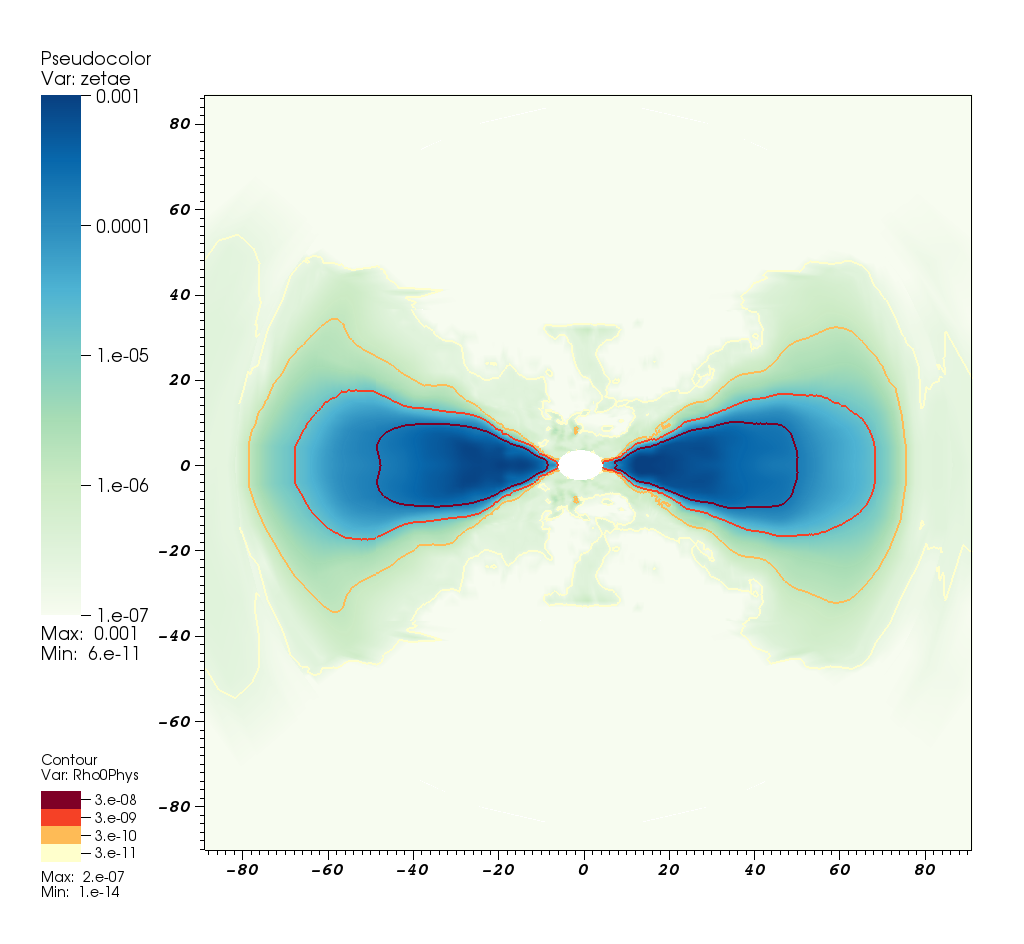
\includegraphics[width=1\linewidth]{Figures/zetae_meridional}
  \end{subfigure}
  \begin{subfigure}{.31\textwidth}
    \centering
    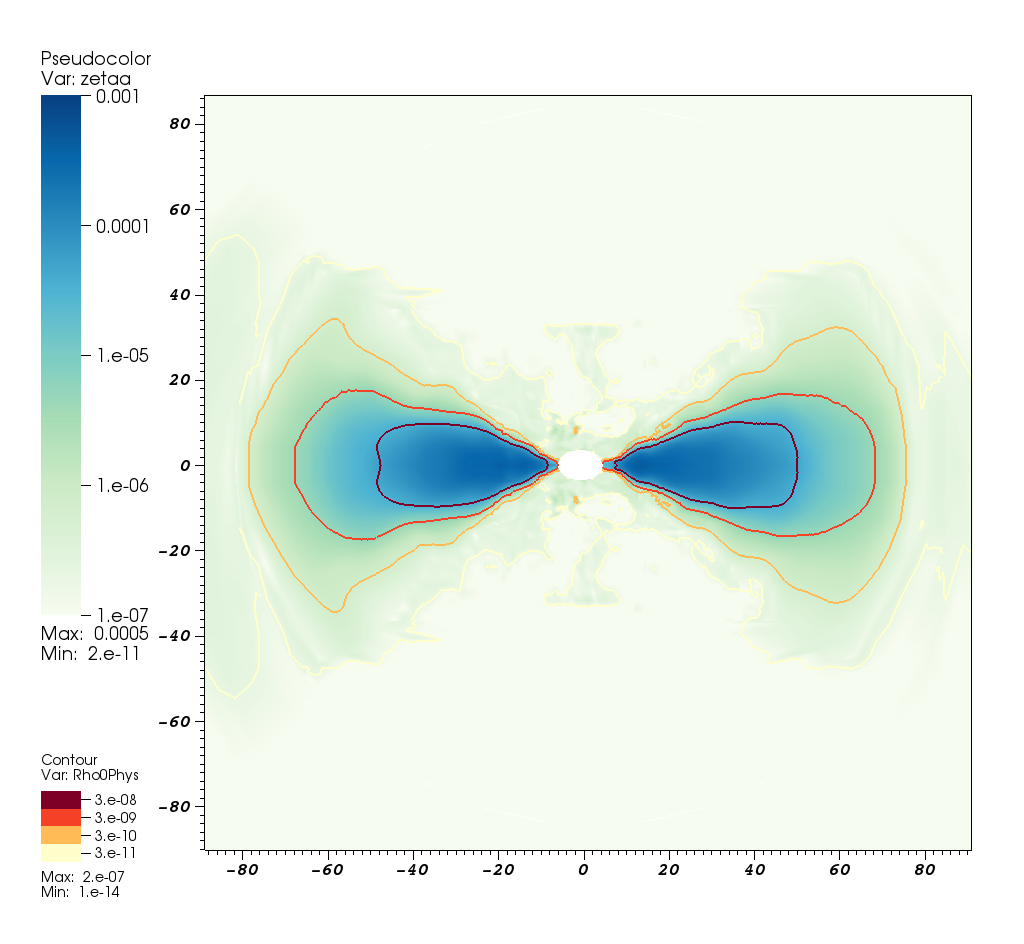
\includegraphics[width=1\linewidth]{Figures/zetaa_meridional}
  \end{subfigure}
  \begin{subfigure}{.31\textwidth}
    \centering
    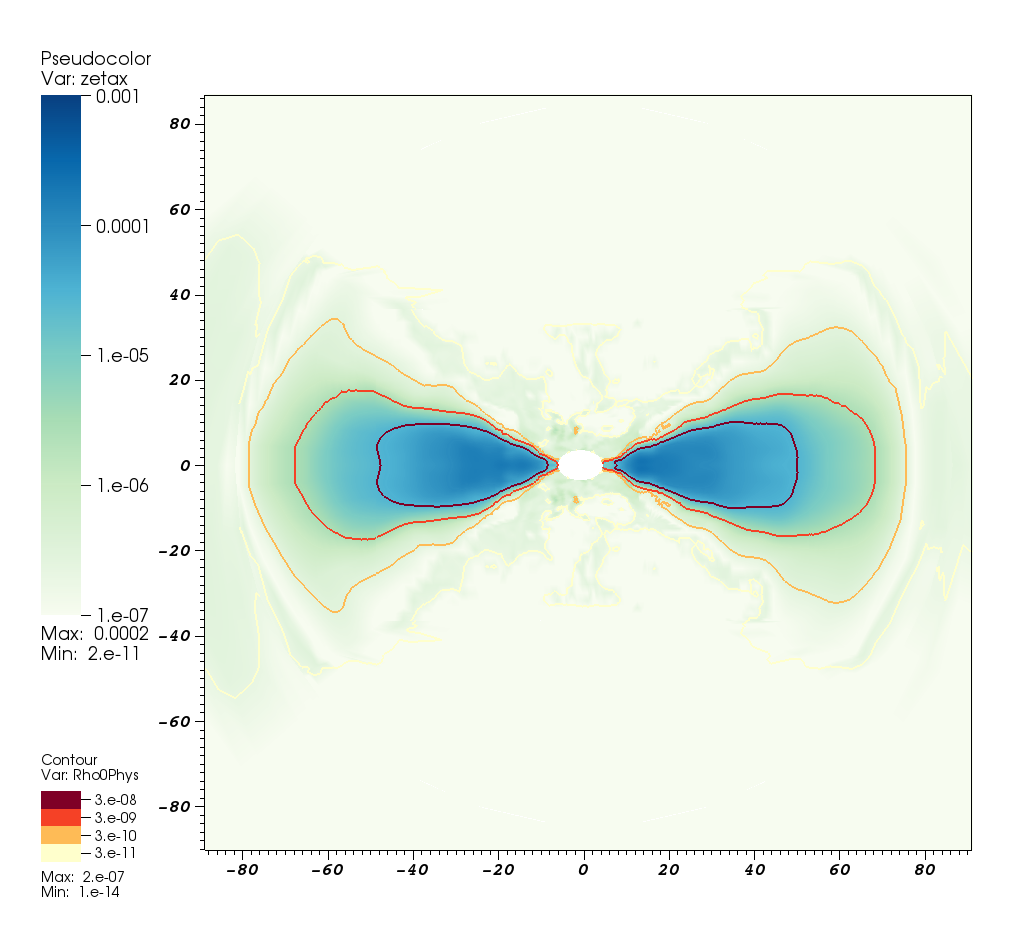
\includegraphics[width=1\linewidth]{Figures/zetax_meridional}
  \end{subfigure}
  \caption[Disk opacities]{
    Meridional slices of disk opacities for each neutrino species,
    $\zeta_{\nu_i}$, in geometrized units of $M_\odot^{-2}$~MeV$^{-1}$.
    The axes are labeled in units of $M_\odot\sim1.5$~km.
    Decadal density contours, in units of $M_\odot^{-2}\sim10^{18}$~g~cm$^{-3}$,
    are provided to give a sense of the matter distribution.
  }
  \label{fig:zeta_meridional}
\end{figure}

\begin{figure}
  \centering
  \begin{subfigure}{.31\textwidth}
    \centering
    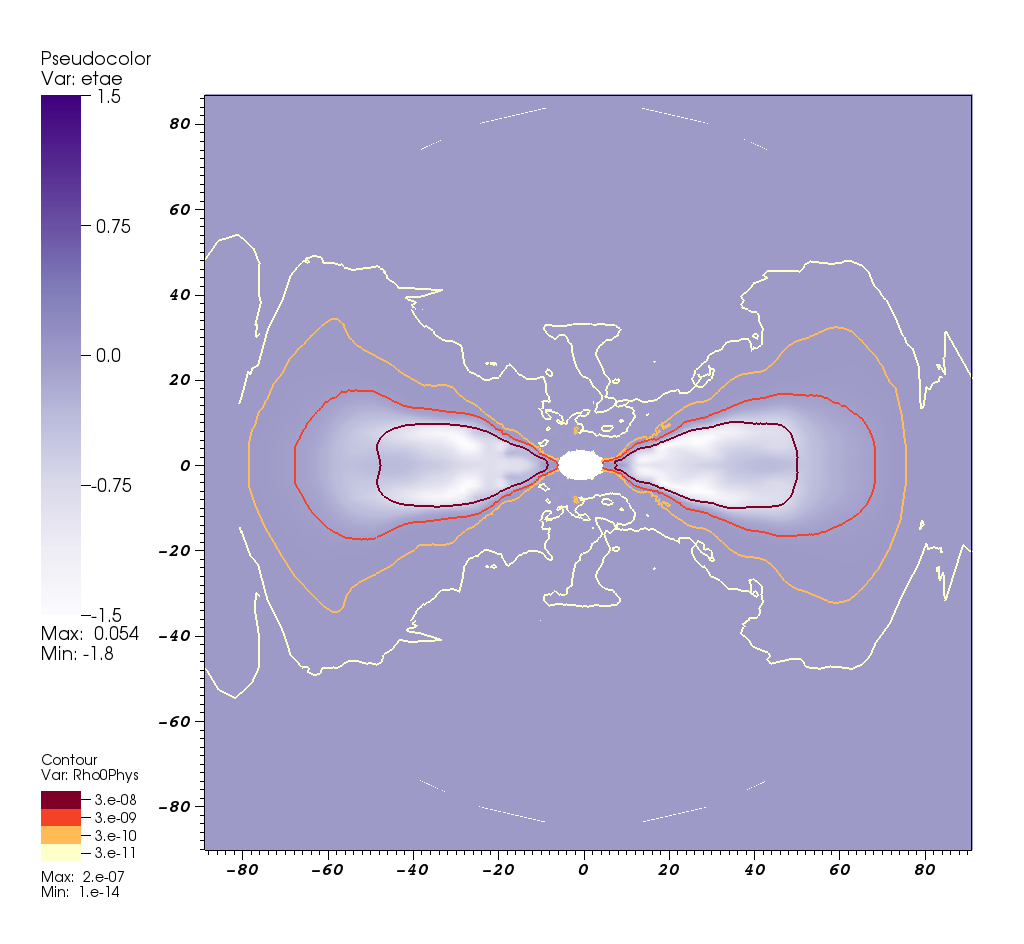
\includegraphics[width=1\linewidth]{Figures/etae_meridional}
  \end{subfigure}
  \begin{subfigure}{.31\textwidth}
    \centering
    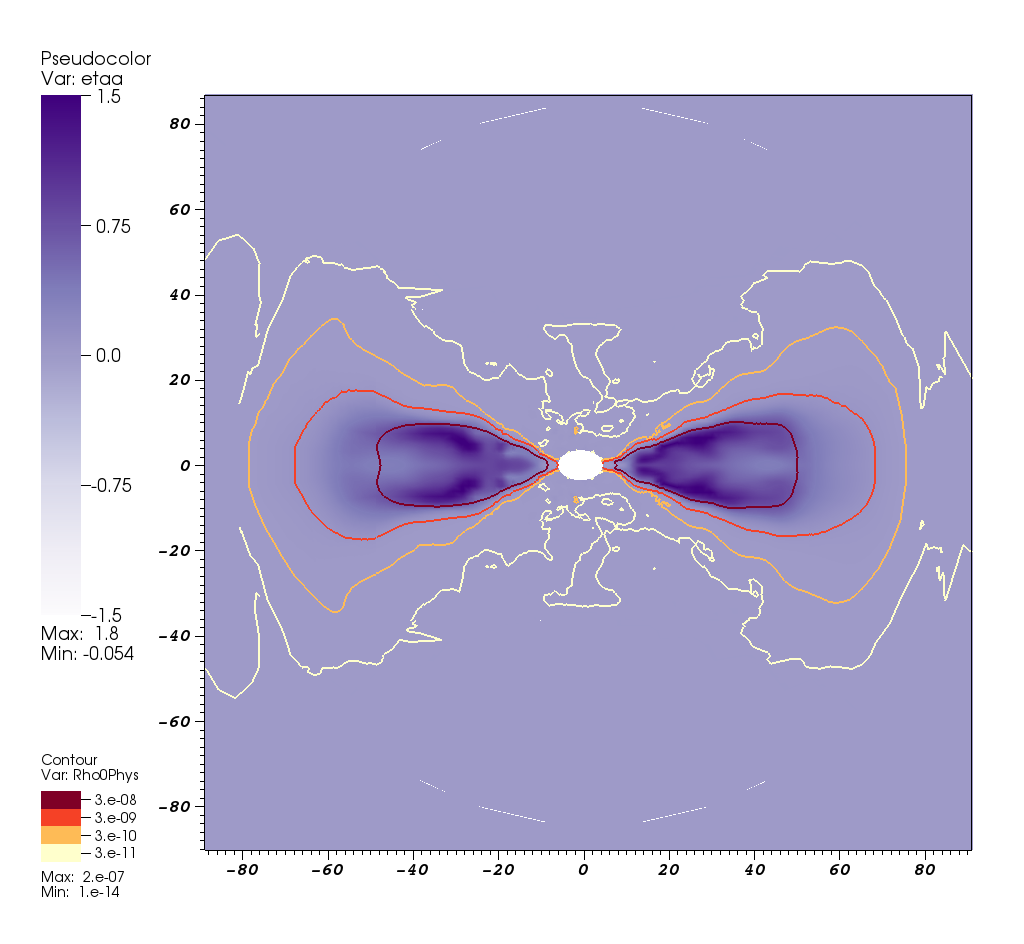
\includegraphics[width=1\linewidth]{Figures/etaa_meridional}
  \end{subfigure}
  \caption[Disk neutrino chemical potentials]{
    Meridional slices of neutrino chemical potentials for $\nu_e$ and
    $\nu_a$. The chemical potential for $\nu_x$ is zero by construction
    in the leakage scheme: the heavy-lepton neutrinos are assumed to
    stream freely.
    The axes are labeled in units of $M_\odot\sim1.5$~km.
    Decadal density contours, in units of $M_\odot^{-2}\sim10^{18}$~g~cm$^{-3}$,
    are provided to give a sense of the matter distribution.
  }
  \label{fig:eta_meridional}
\end{figure}

\subsubsection{From the Equator}
\label{sssc:f_this_case_E}

In Figs.~\ref{fig:f_disk_eq_13MeV}~and~\ref{fig:f_disk_eq_34MeV} I display
$f_\nu(\Omega_i)$ over the whole sky, as viewed from the equator, at the
same characteristic energies as in
Figs.~\ref{fig:f_disk_axis_13MeV}~and~\ref{fig:f_disk_axis_34MeV}.

\begin{figure}
  \centering
  \begin{subfigure}{.3\textwidth}
    \centering
    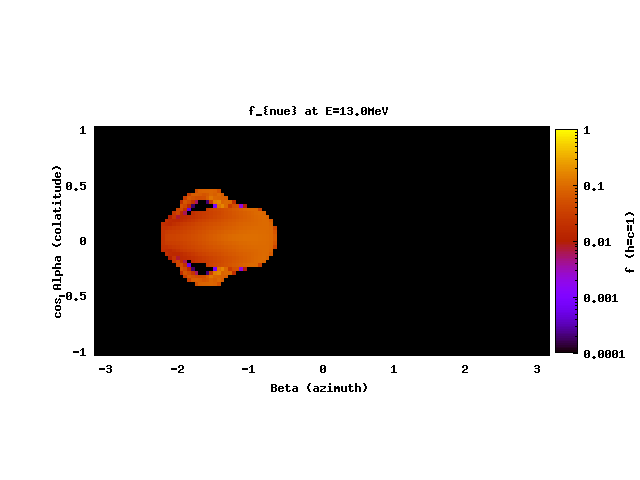
\includegraphics[width=1\linewidth]{Figures/f_nue-E-13MeV}
  \end{subfigure}
  \begin{subfigure}{.3\textwidth}
    \centering
    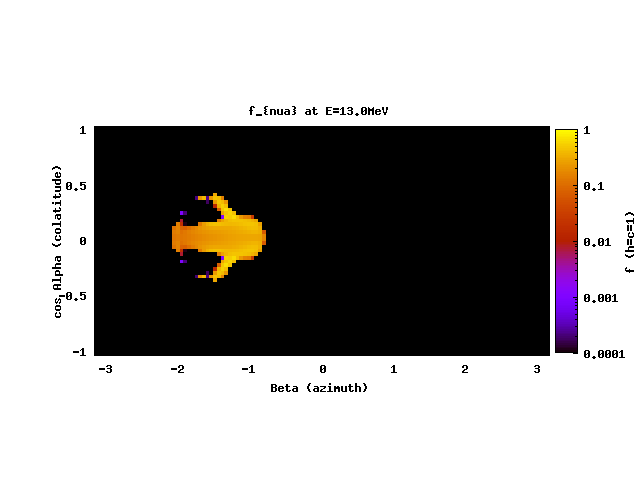
\includegraphics[width=1\linewidth]{Figures/f_nua-E-13MeV}
  \end{subfigure}
  \begin{subfigure}{.3\textwidth}
    \centering
    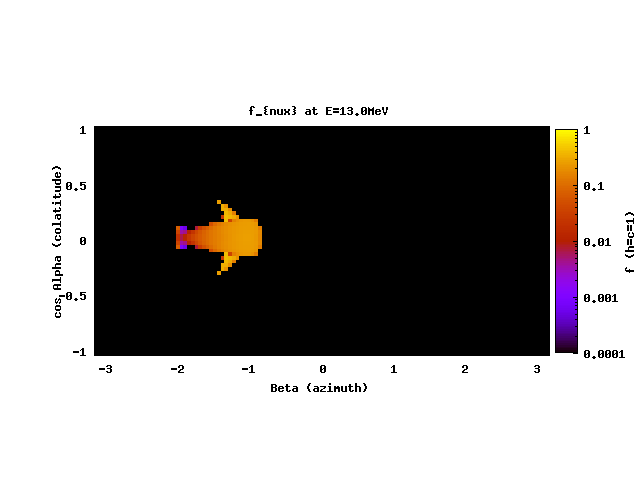
\includegraphics[width=1\linewidth]{Figures/f_nux-E-13MeV}
  \end{subfigure}
  \caption[$f_\nu$ for the disk, from the equatorial plane: sky map at average energy]{
    Neutrino distribution functions from the accretion disk over the sky in a
    single energy band, $p_t=13$~MeV. The observer is stationary in the
    equatorial plane at coordinate radius 120~km from the black hole.
    The panels from left to right depict $f_{\nu_e}$, $f_{\nu_a}$,
    and $f_{\nu_x}$.
  }
  \label{fig:f_disk_eq_13MeV}
\end{figure}

\begin{figure}
  \centering
  \begin{subfigure}{.3\textwidth}
    \centering
    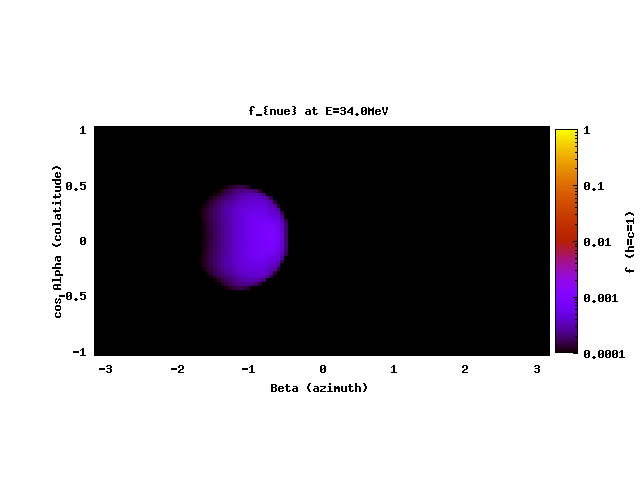
\includegraphics[width=1\linewidth]{Figures/f_nue-E-34MeV}
  \end{subfigure}
  \begin{subfigure}{.3\textwidth}
    \centering
    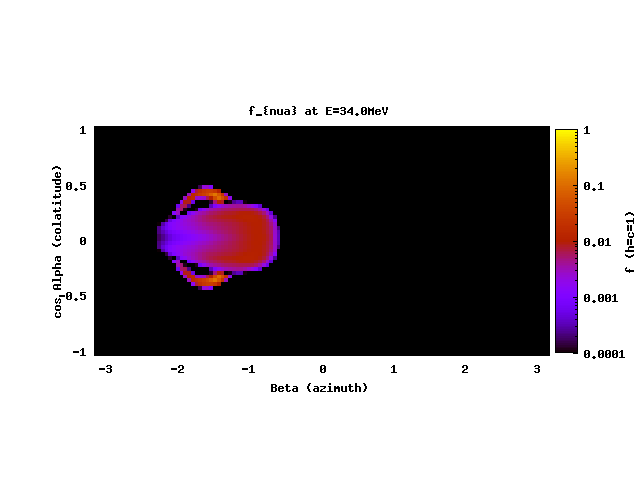
\includegraphics[width=1\linewidth]{Figures/f_nua-E-34MeV}
  \end{subfigure}
  \begin{subfigure}{.3\textwidth}
    \centering
    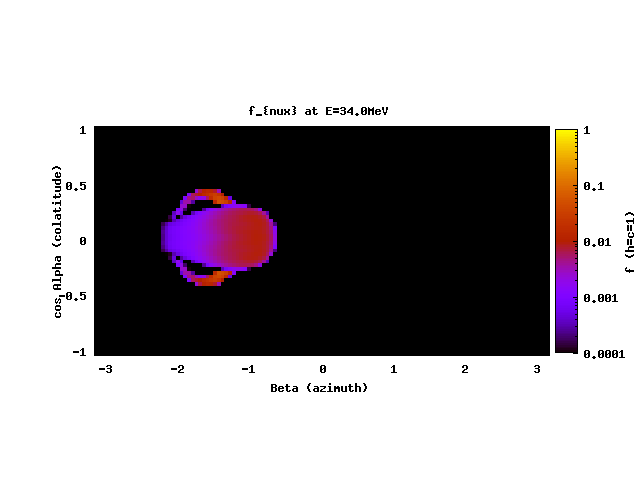
\includegraphics[width=1\linewidth]{Figures/f_nux-E-34MeV}
  \end{subfigure}
  \caption[$f_\nu$ for the disk, from the equatorial plane: sky map at high energy]{
    Same as Fig.~\ref{fig:f_disk_eq_13MeV}, but in the energy band $p_t=34$~MeV.
    Left to right, the panels depict $f_{\nu_e}$, $f_{\nu_a}$, and $f_{\nu_x}$.
  }
  \label{fig:f_disk_eq_34MeV}
\end{figure}

Several observations:
\begin{enumerate}
  \item The back side of the neutrinosurface, behind the black hole, is visible
    as a ring on the top and bottom of the image.
    This is due to the bending of rays by the spacetime curvature of the black
    hole. This has the effect of enlarging the emission surface compared to
    that obtained by a simple Newtonian calculation, an effect seen even in
    the simple case of the hot compact star (Fig.~\ref{fig:f_hot_ns}).
    See Fig.~\ref{fig:schematic_ray_bending} for an explanatory cartoon.
  \item The left side of the neutrinosurface---which is actually the right
    side of the disk in physical space (the image is reflected vertically and
    horizontally, as by a pinhole camera)---is less intense. In the cases of
    $f_{\nu_a}$ and $f_{\nu_x}$, it actually vanishes at low energy.
    This is due to the relativistic fluid velocities: the left side of the disk
    image is moving away from, and the right side toward the viewer.
    See Fig.~\ref{fig:schematic_ray_doppler} for an explanatory cartoon.
    Neutrinos emitted from the left side are doppler shifted to lower energies
    than those from the right side. At these energies,
    $p_t\gtrsim\langle\varepsilon_\nu\rangle$,
    this has the effect of decreasing the intensity, i.e.\ decreasing
    $f_\nu(p_t)$.
    The effect is reversed at energies for which
    $\partial_{p_t}f_\nu(p_t)>0$.
  \item The image of the disk is offset to the left. This is an effect of the
    rotation of the central black hole, which communicates a sympathetic spin
    to the spacetime. This is a well-known and experimentally-verified effect
    \todo{ref theory and GravB}
    called frame dragging, or gravitomagnetism.
    According to a viewer at rest very far away from the disk, neutrinos
    streaming away from its surface follow trajectories curving away from
    the spin of the black hole, forming a whirlpool shape.
    \todo{add cartoon or computed ray trajectories}
\end{enumerate}

\begin{figure}
  \centering
  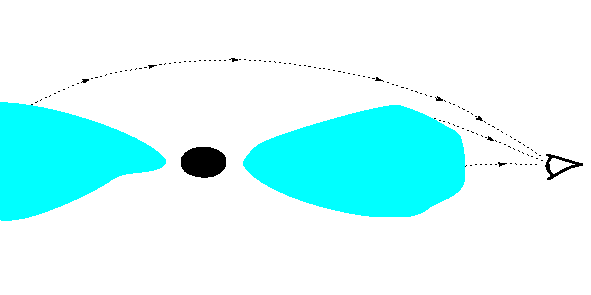
\includegraphics[width=10cm]{Figures/seeing_back_of_disk}
  \caption[Cartoon of neutrino rays bending over the disk]{
    Cartoon showing how a viewer (on the right) can see parts of the
    neutrinosurface that would be obscured in Euclidean geometry.
    This is a meridional slice of the disk. The fluid is shown in blue, the
    black hole is black, and several neutrino trajectories are shown as dashed
    lines.
  }
  \label{fig:schematic_ray_bending}
\end{figure}

\begin{figure}
  \centering
  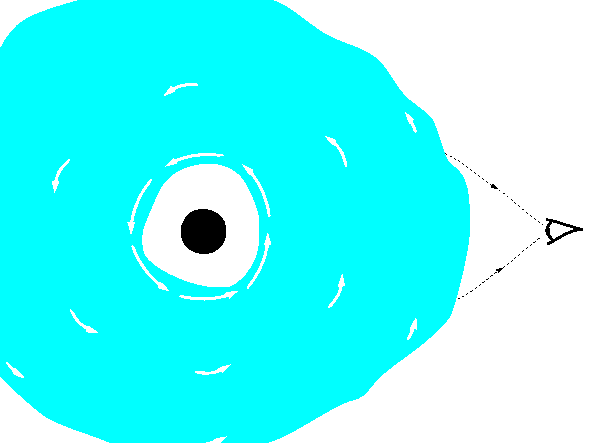
\includegraphics[width=10cm]{Figures/seeing_disk_doppler_shift}
  \caption[Cartoon of the doppler shift due to disk rotation]{
    Cartoon showing how a viewer (on the right) experiences a differential
    doppler shift. This is an equatorial slice of the disk.
    The fluid is shown in blue and its velocity field by white arrows, longer
    representing faster. The black hole is black, and two neutrino trajectories
    are shown as dashed lines. The left side of the disk (downward in the
    cartoon) is moving roughly toward the viewer, boosting its neutrino emission;
    the opposite is true of the right side of the disk.
    Furthermore, the differential rotation of the disk makes this effect more
    pronounced for neutrinosurfaces deeper within the disk.
  }
  \label{fig:schematic_ray_doppler}
\end{figure}

\section{Calculating $q_{\nu \bar{\nu}}$}
\label{sec:q_algorithm}
The standard model for gamma ray bursts consists of an ultrarelativistic jet
driven by rapid accretion onto a stellar-mass black hole. One of the missing
links in this model is the physical mechanism connecting the accretion to the
jet. How does the gravitational energy released by the transport of matter
toward and eventually into the black hole end up powering a highly-collimated
low-density plasma moving away from the black hole with a Lorentz factor of
10s or 100s? The link likely takes the form of one or both of the following
processes:
\begin{itemize}
  \item \emph{Magnetic fields}: If there are strong magnetic fields present, the
    Blandford-Znajek process \citep{blan1977-blandford_znajek} can extract
    rotational energy from the black hole and accelerate plasma out along its
    rotation axis. Additionally, magnetic fields in the accretion disk may
    centrifugally accelerate plasma, tapping the rotational energy of the
    disk itself \citep{blan1982-blandford_payne}.
  \item \emph{Neutrino heating}: Highly energetic neutrino-antineutrino pairs
    can annihilate into into electron-positron pairs
    ($\nu \, \bar{\nu} \rightarrow e^{-} \, e^{+}$)
    with excess energy from the interaction going into the kinetic energy of the
    lepton pair.
    This process is particularly efficient at high neutrino energies and large
    collision angles, conditions found in the funnel of the accretion disk.
    This $e^{-}\,e^{+}$ gas rapidly thermalizes via electromagnetic interactions,
    and the superheated plasma expands away from the disk explosively. The inner
    walls of the funnel may act to confine the plasma, collimating it into a jet.
\end{itemize}

Simulations indicate that the first process is extremely sensitive to the
\todo{ask fatemeh for ref}
initial magnetic field configuration, with no jet structure forming if there is
no initially large-scale poloidal field in the accretion disk.
I won't explore the magnetic processes further here.

The second process is sensitive to the geometry and spectrum of the emission
\todo{cite geneology of $\nu\bar{\nu}$ studies}
and in the context of neutron star--black hole mergers, has only been studied
in highly-idealized models of analytical accretion disks or Newtonian gravity.
\todo{maybe add technical specs of GRBs and nuclear accretion sites}

Let us explore the viability of the neutrino-antineutrino annihilation process
in the case of the accretion disk presented in Chap.~\ref{chap:leakage}.

\subsubsection{Brief History of Neutrino-Antineutrino Annihilation Studies}
\label{sssc:nunubar_review}
In the late 1980s, \cite{good1987-nunubar} and \cite{bere1987-nunubar}
\todo{fix cite}
independently proposed neutrino-antineutrino annihilation as a process that could
transfer a fraction of the neutrino energy released by stellar collapse, as in
Type II supernovae, into an electron-positron pair plasma. Their calculations
were performed assuming Newtonian gravity, but they found efficiencies of a
fraction of a percent of the total neutrino luminosity.
\todo{add paczynski 1990}
\todo{add Meszaros \& Rees 1992}

\cite{salm1999-nunubar} examined the same process in a general relativistic
\todo{fix cite}
formulation and discovered and enhancement of efficiency to a few percent.
They assumed a Schwarzschild geometry, a spherical emitter, and a Fermi-Dirac
\todo{check}
neutrino spectrum.

\cite{asan2000-nunubar} studied the same process in a Schwarzschild geometry,
\todo{fix cite}
examining both a spherical and disk emitter, and considering the
redshift of energy as its carrier travels away from the gravitational source.
They found that gravitational bending of rays enhances, but gravitational
redshift suppresses the efficiency of the process by about the same factor,
bringing efficiencies back down to a fraction of a percent.
\todo{check}

\cite{ruff1999-nsns_i,ruff1999-nsns_ii,ruff1999-nsns_iii} and
\cite{ross2003-nsns_i,ross2003-nsns_ii,ross2003-nsns_iii} innaugurated the
\todo{fix cites}
construction of realistic neutron star--neutron star merger models, using
three-dimensional hydrodynamical simulations.
They used pseudo-Newtonian gravitational potentials and also found a
neutrino-antineutrino annihilation efficiency of fractions of a percent,
insufficient to power all but the least-energetic of the observed
short gamma ray bursts.
\todo{point out approximate calc of $q_{\nu\bar{\nu}}$}

\cite{seti2006-nunubar} used one of the disk models computed in
\cite{ruff1999-nsns_i}
\todo{fix cites}
as the initial configuration for pseudo-Newtonian simulations of the
accretion disk's evolution, varying phenomenological parameters like inner disk
radius (as a proxy for black hole spin) and viscosity (related to the
accretion rate). Only in their most optimistic cases (high spin, high
accretion rate) did they find annihilation
efficiencies that could release GRB-equivalent energies.

\cite{birk2007-nunubar} examined the process for four different phenomenological
\todo{fix cite}
emission geometries, embedded in a Kerr spacetime, varying the spin of the
central black hole. They found that spin effects could enhance the annihilation
efficiency by a factor of 2, and cautiously concluded that from their most
optimistic models, neutrino-antineutrino annihilation alone could account for
even the most distant GRBs.
\todo{isn't it least energetic GRBs?}

\cite{hari2010-nunubar} examined this process in the context of collapsars,
\todo{fix cite}
the leading model for long gamma ray bursts. They developed a ray tracing code,
solving the Boltzmann equation around an accretion disk formed in a massive
stellar collapse. Their results, however, were relevant to energy deposition
in the star, to drive the explosion, not to jet energetics.

\cite{zala2011-nunubar} used ray tracing in analytical disk models, assuming
\todo{fix cite}
all neutrinos were emitted from a single neutrinosurface, and no scattering
occured after emission. They derived a scaling between annihilation deposition
energy, black hole spin, and accretion rate for their models. For nearly
extremal spins and large accretion rates, they estimated this process was
sufficient to generate GRBs with the observed energies.

\subsection{Neutrino-Antineutrino Annihilation Equations}
\label{ssec:nunubar_integral}
Our goal is to calculate the total heating rate, $Q_{\nu \bar{\nu}}$ (erg~s$^{-1}$)
due to $\nu\,\bar{\nu} \rightarrow e^{-}\,e^{+}$ by summing up the contributions
of the deposition rate per volume for this process,
$q_{\nu \bar{\nu}}(x^\alpha)$:
\begin{equation}
  \label{eqn:Q_vol}
  Q_{\nu \bar{\nu}} \equiv \int \diff^3 x\,q_{\nu \bar{\nu}}(x^\alpha)
\end{equation}
$q_{\nu \bar{\nu}}(x^\alpha)$ is an inherently frame-dependent quantity but is
\todo{add redshift factor for time}
analogous to the frame-independent annihilation rate per volume,
$n_{\nu \bar{\nu}}(x^\alpha)$:
\begin{equation}
  n_{\nu \bar{\nu}}(x^\alpha) \equiv
  \frac{\diff N}{\diff \bar{t} \, \diff \bar{V}} =
  c \frac{\diff N}{\sqrt{-\psi}\,\diff^4 x}
\end{equation}
where $\psi$ is the determinant of the 4-metric, and we have defined
$n_{\nu \bar{\nu}}$ in the first expression in an orthonormal tetrad erected at
$x^\alpha$. In the second expression we have written it in general curvilinear
coordinates, emphasizing its Lorentz invariance: it is composed of scalars
particle number and proper volume. $\diff^4 x$ are the contravariant components
of the spacetime volume, in cartesian coordinates
$\diff t \, \diff x \, \diff y \, \diff z$.

The annihilation rate is written in a tetrad as \cite{goodman87}:
\todo{fix cite}
\begin{align}
  \label{eqn:qdot_orig}
  n_{\nu \bar{\nu}}(x^\alpha)
  &= \int \diff^3p_{\nu} \diff^3p_{\bar{\nu}} \,\,
  f_{\nu}(x^j;p_{\nu k})
  f_{\bar{\nu}}(x^j;p_{\bar{\nu} k})
  \sigma |v_\nu-v_{\bar{\nu}}| \nonumber \\
  &= \int \diff^3p_\nu \diff^3p_{\bar{\nu}} \,\,
  f_{\nu}(x^j;p_{\nu k})
  f_{\bar{\nu}}(x^j;p_{\bar{\nu} k})
  \frac{\sigma c}{p_{\nu}^t p_{\bar{\nu}}^t} (p_{\nu \alpha}  p_{\bar{\nu}}^\alpha) \nonumber \\
  &= \int \diff^3p_{\nu} \diff^3p_{\bar{\nu}} \,\,
  f_{\nu}(x^j;p_{\nu k})
  f_{\bar{\nu}}(x^j;p_{\bar{\nu} k})
  \frac{2 c^3 K G_F^2}{p_{\nu}^t p_{\bar{\nu}}^t}
  (p_{\nu \alpha} p_{\bar{\nu}}^\alpha)^2
\end{align}
\todo{clean up/simplify}
where $\diff^3p$ are the covariant components of the spatial momentum volume,
$\diff p_x \diff p_y \diff p_z$.
Eqn.~\ref{eqn:qdot_orig} is covariant since all of its constituents are
invariants: $f_\nu$, $\diff^3p/p^t$, and $(p_{\nu \alpha} p_{\bar{\nu}}^\alpha)$.
\todo{ref Chap.~\ref{chap:intro}}

$K$ is given in the Standard Model as:
\begin{equation}
  K \left\{{e \atop \mu \, \tau}\right\} = \frac{1}{6\pi}
  (1 \, \left\{{+ \atop -}\right\}
  \, 4 \sin^2 \theta_w + 8 \sin^4 \theta_w) \nonumber
\end{equation}
where the upper (lower) sign is used for light (heavy) lepton neutrinos,
the difference arising because only $e$-type neutrinos can interact with
matter via the charged-current at energies less than $m_\mu\sim100$~MeV
and $m_\tau\sim2000$~MeV.
\todo{is this right?}
The Fermi constant is $G_F^2 = 5.29 \times 10^{-44} \text{cm}^2 \text{MeV}^{-2}$,
and the Weinberg angle is $\sin^2 \theta = 0.23$.
\todo{cite constants}

To calculate $q_{\nu \bar{\nu}}(x^\alpha)$ we weight the kernel in
Eqn.~\ref{eqn:qdot_orig} by the total energy of the neutrinos
$\varepsilon_{\nu} + \varepsilon_{\bar{\nu}}$ \cite{asano00, salmonson99}.
\todo{fix cites}
Since the energy is only one component of a proper 4-vector, this becomes an
inherently frame-dependent calculation.
(Alternatively we could weight the kernel by the total 4-momentum of the
neutrinos, but that would increase our computational work by a factor of 4.)

So which observer makes sense for this calculation? That depends. Since we are
asking how much energy is available to power a relativistic jet which eventually
shocks into the interstellar medium far away from the gravitational
neighborhood of the emitter, we want to account for
the redshift losses to the energy. So we weight our kernel by
$\varepsilon=-p_t c$, the energy redshifted to infinity, because the metric in
our numerical coordinates is stationary and asymptotically flat.
If, however, we were asking how much energy to add as a source term in the
hydrodynamic equations, to compute the evolution of the shock, we would weight
our kernel by a local energy $\varepsilon=-p_\alpha u^\alpha$, the energy
measured in the fluid rest frame. For notational simplicity, we use
$\varepsilon$ to represent the first choice in the following calculations.

So the heating rate at $x^\alpha$ measured by an observer at infinite distance is
\begin{equation}
  \label{eqn:qdot}
  q_{\nu \bar{\nu}}(x^\alpha)
  = A \int \diff^3p_{\nu} \diff^3p_{\bar{\nu}} \,\,
  f_{\nu}(x^j;p_{\nu k})
  f_{\bar{\nu}}(x^j;p_{\bar{\nu} k})
  \frac{  \varepsilon_{\nu}+\varepsilon_{\bar{\nu}}}{p_{\nu}^t p_{\bar{\nu}}^t}
  (p_{\nu \alpha} p_{\bar{\nu}}^\alpha)^2
\end{equation}
where we have defined $A \equiv 2 c^3 K G_F^2$ and $\varepsilon$ as described above.

To compute the integral in general curvilinear coordinates we first write the
momenta in Eqn.~\ref{eqn:qdot} in spherical polar components
$\{p_t,p_r,p_{\theta},p_{\phi}\}$ (see Fig.~\ref{fig:p_conventions}).
The volume element in momentum space is
$\diff^3p\equiv\diff p_x\wedge\diff p_y\wedge\diff p_z=\left|\frac{\partial(p_r,p_\theta,p_\phi)}{\partial(p_x,p_y,p_z)}\right|\diff p_r\wedge\diff p_{\theta}\wedge\diff p_{\phi}$.
\todo{clarify}

Eqn.~\ref{eqn:qdot} becomes
\begin{align}
  \label{eqn:qdot_general_orig}
  q_{\nu \bar{\nu}}(x^\alpha)
  &= A \int \diff p_{\nu r} \diff p_{\bar{\nu} r} \,\,
  p_{\nu r}^2 \diff\Omega_{\nu} p_{\bar{\nu} r}^2 \diff\Omega_{\bar{\nu}} \,\,
  f_{\nu}(x^j;p_{\nu k}) f_{\bar{\nu}}(x^j;p_{\bar{\nu} k})
  \frac{\varepsilon_{\nu} + \varepsilon_{\bar{\nu}}}{p_{\nu}^t p_{\bar{\nu}}^t}
  (p_{\nu \alpha} p_{\bar{\nu}}^\alpha)^2
\end{align}

Furthermore, employing the momentum relations from Sec.~\ref{ssec:p_conventions}
we can write Eqn.~\ref{eqn:qdot_general_orig} explicitly in terms of energy
scale and direction:
\begin{equation}
  \begin{split}
    \label{eqn:qdot_general}
    q_{\nu \bar{\nu}}(x^\alpha)
    &= A \int \diff p_{\nu t} \diff p_{\bar{\nu} t} \,\,
    \diff (\cos \alpha_{\nu}) \diff (\cos \alpha_{\bar{\nu}}) \,\, \diff \beta_{\nu} \diff \beta_{\bar{\nu}} \\
    & \qquad \qquad \qquad
    \times f_{\nu}(x^j;p_{\nu t},\Omega_{\nu})
    f_{\bar{\nu}}(x^j;p_{\bar{\nu} t},\Omega_{\bar{\nu}}) \\
    & \qquad \qquad \qquad
    \times \frac{(\varepsilon_{\nu} + \varepsilon_{\bar{\nu}})(p_{\nu t} p_{\bar{\nu} t})^2}
           {p_{\nu}^t p_{\bar{\nu}}^t} \\
           & \qquad \qquad \qquad
           \times \frac {(p_{\nu \alpha} p_{\bar{\nu}}^\alpha)^2}
                  {(C(\Omega_{\nu k})C(\Omega_{\bar{\nu} k}))^3}
  \end{split}
\end{equation}

The only terms not chosen explicitly, $p_{\nu \alpha} p_{\bar{\nu}}^\alpha$
and $p^t$, are calculated with the help of the metric.

To sum this integral at a single point $x^\alpha$,
we sample the integrand in the 6-dimensional space:
$p_{\nu t}$,
$p_{\bar{\nu} t}$,
$\cos \alpha_{\nu}$,
$\cos \alpha_{\bar{\nu}}$,
$\beta_{\nu}$,
$\beta_{\bar{\nu}}$.
We integrate over $\cos \alpha$ in order to distribute rays isotropically over
the sky.

\subsection{Monte Carlo Integration of $q_{\nu\bar{\nu}}$}
\label{ssec:monte_carlo}
The numerical solution to Eqn.~\ref{eqn:qdot_general} is a sum over
six dimensions, a steep computational challenge.
A straightforward trapezoidal integration with a grid of only 10
points along each dimension requires $10^6$ samples of $f_\nu$ and
$f_{\bar{\nu}}$, each requiring a separate geodesic integration possibly
requiring as much as $\sym0.1$~s;
on one processor this would take a day of walltime.
Additionally, a resolution of only 10 points per dimension introduces large
errors to our estimate; but doubling our resolution increases the wall time
by a factor of $2^6$, to several months.
Furthermore, we aim to repeat this calcultion at many points throughout the
spatial volume to compute $Q_{\nu\bar{\nu}}$ (Eqn.~\ref{eqn:Q_vol}).

One solution is to parallelize over rays, but before we follow that lead, we
can formulate the integration more efficiently.
One guiding clue to overcoming the challenge is that most of these $N$
samples would contribute very little or nothing to the total integral.
An adaptive Monte Carlo integration technique is ideal for such problems.
We employ the Vegas algorithm
(described in detail in \citealt[Sec.~7.9]{pres2007-nr_3rd_ed}),
which specifies a procedure to randomly sample the integration space:
homogeneously at first, then in iterated stages preferring more and more
heavily those regions that contribute most to the integral.
In tests with analytic integrands mimicking the expected distribution functions,
I found the numerical estimate to converge to the true integral faster than
$N^{1/2}$, as expected for a statistical estimate. These tests required
$N\sim10^4$ for 10\% accuracy.

The range of the energy integration must capture the major contributions to the
integral, and not be so large that the adaptive algorithm has difficulty
finding the important range at an early stage.
\todo{add notes on energy bounds from equations.tex}

\subsection{Code Tests of $q_{\nu\bar{\nu}}$}
\label{ssec:q_tests}
I implemented the Monte Carlo integration of $q_{\nu\bar{\nu}}$ as a driver
around the matter ray tracing code described in Sec.~\ref{sec:f_algorithm},
using code freely available in the open source GNU Scientific
Libary\footnote{\url{http://www.gnu.org/software/gsl/}}.
Rather than compute the integral with a pre-specified number of samples, $N$,
the algorithm proceeds iteratively until its error estimate falls below
a pre-specified accuracy threshold.
The error is estimated, in the Vegas framework, from the variance in the
samples of the integrand. 

To test the integration let us revisit the toy models from
Sec.~\ref{ssec:f_tests}.

\subsubsection{Homogeneous Minkowski}
\label{sssc:q_homo_mink}
We may analytically compute $q_{\nu\bar{\nu}}$ in the homogeneous emitting
medium in flat spactime presented in Sec.~\ref{sssc:f_homo_mink}.
\todo{add notes from *.nb}

\begin{figure}
  \centering
  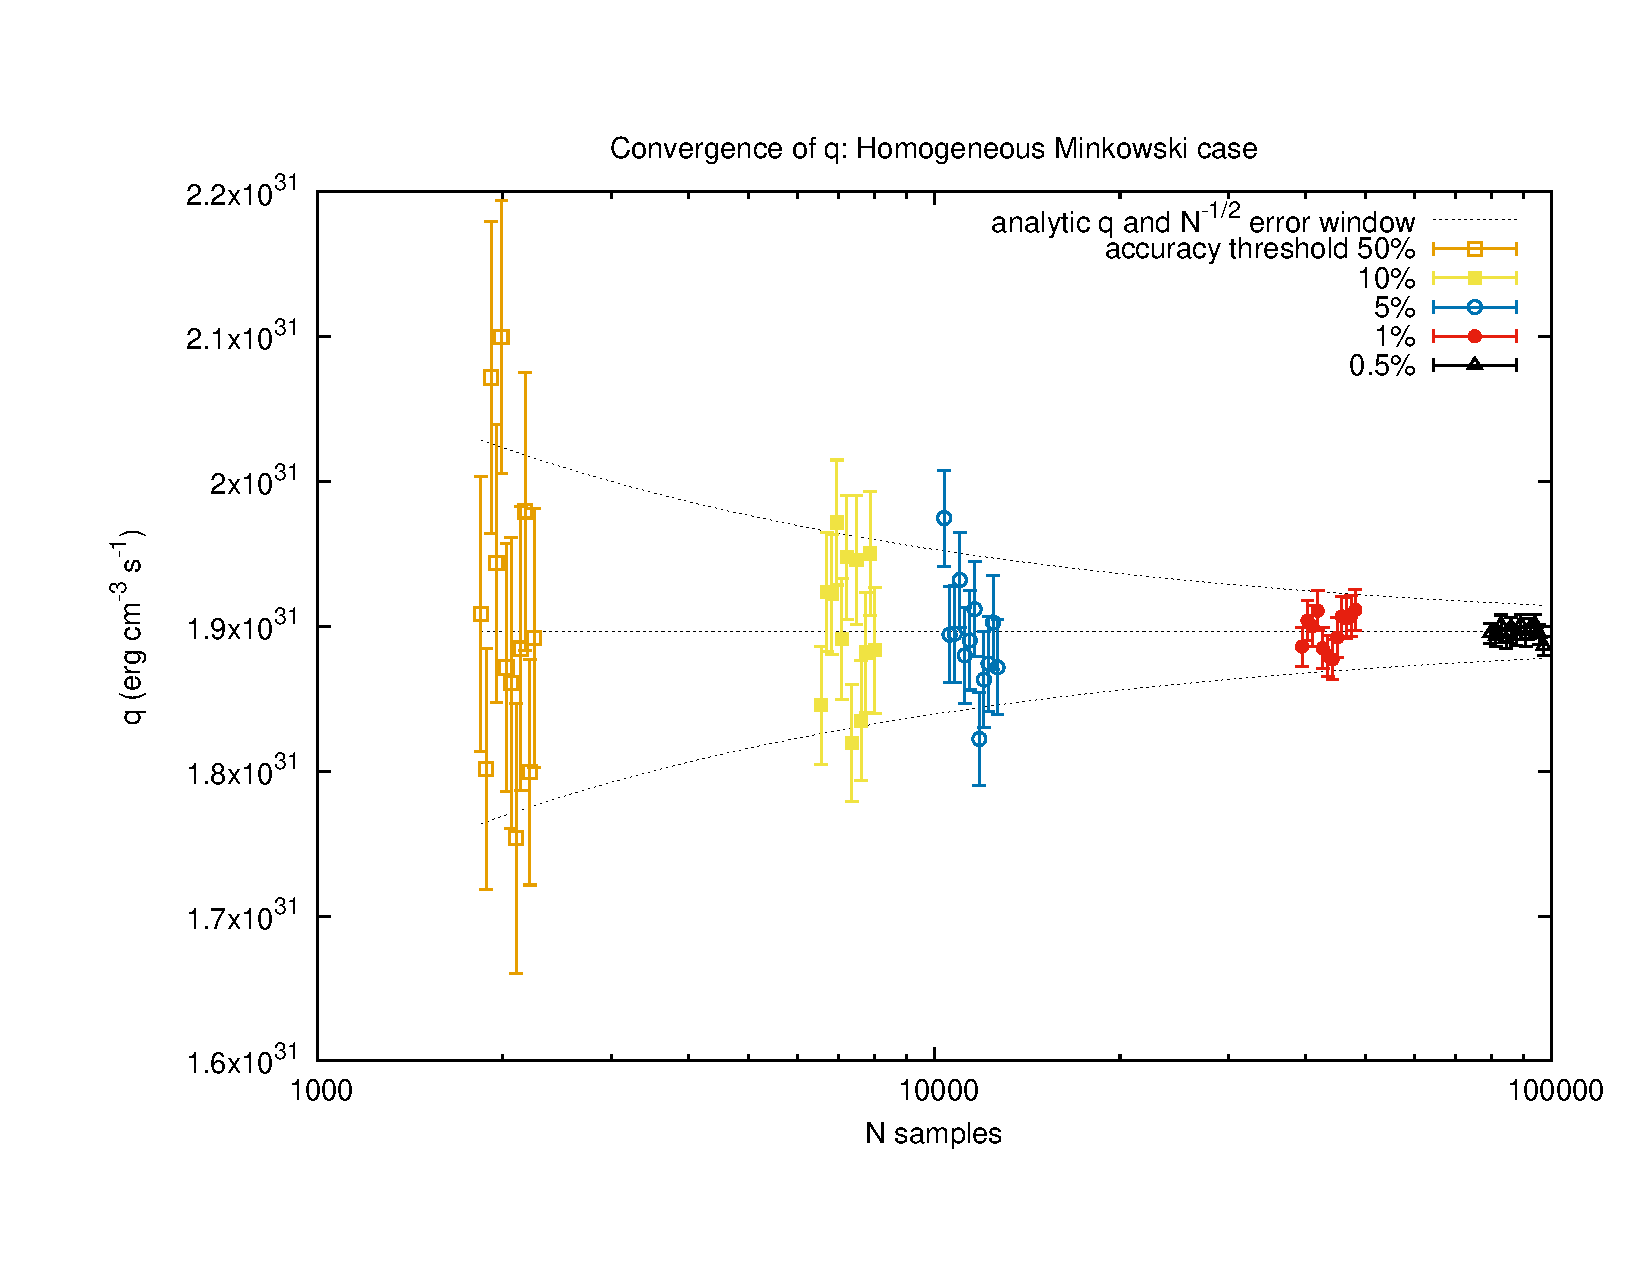
\includegraphics[width=16cm]{Figures/convergence_homogeneous_minkowski}
  \caption[Convergence of $q_{\nu\bar{\nu}}$ in the homogeneous Minkowski case]{
    Convergence of the integration estimating $q_{\nu\bar{\nu}}$ in the
    homogeneous Minkowski case.
    The horizontal axis is the number of samples of the integrand, $N$;
    the number of unique rays traced, therefore, is $2N$.
    At four different accuracy thresholds (the four clusters), I have computed
    the integral 12 times, to display the statistical scatter.
    The Vegas estimates of the error are given as as error bars.
    The legend labels each group of points by the accuracy threshold; but note,
    at low accuracy, the algorithm is bad at guessing how many samples it needs,
    so the threshold and the final error estimate disagree at low-$N$.
    The 12 points in each cluster are plotted with a small, false scatter in $N$
    to make them visually distinct.
    The dashed lines show the correct value of $q_{\nu\bar{\nu}}$ and an
    $N^{1/2}$-envelope (with an arbitrary vertical scaling to bound the points
    at the highest resolutions).
  }
  \label{fig:convergence_homo_mink}
\end{figure}

Fig.~\ref{fig:convergence_homo_mink} shows the results of a suite of
computations at increasing accuracy thresholds.
The numerical estimate of $q_{\nu\bar{\nu}}$ converges to the analytical result
faster than $N^{1/2}$ (the dotted envelope in the figure).
For an accuracy of 10\% (in this simple case) we need to compute
$\sym3\times10^3$ samples of the integrand.

\subsubsection{Hot Compact Star}
\label{sssc:q_af_sphere}
We may also analytically compute $q_{\nu\bar{\nu}}$ outside the hot compact
star presented in Sec.~\ref{sssc:f_af_sphere}.
\todo{add notes from *.nb}
In that Section, we identified a spurious
variation in $f_\nu$ across the neutrinosurface (seen in
Fig.~\ref{fig:f_hot_ns}), due to the combination of a discrete jump in opacity
at the surface, and the finite time steps used to integrate the rays
(discussed in Sec.~\ref{ssec:timestepping}).
In the integral of $q_{\nu\bar{\nu}}$ presented here, our standard settings
for the Dormand-Prince time stepping (throttling $\Delta t\leq1.5\,M_\odot$)
introduce a systematic error of 10--20\% in the integral which does not converge
away with $N$, the number of rays traced.
In order to push this systematic error in $f_\nu$ low enough to examine the
error in our Monte Carlo algorithm for $q_{\nu\bar{\nu}}$,
we have throttled the time stepping to $\Delta t \leq0.1\,M_\odot$.
At the standard timestep settings, sampling the integrand $6\times10^4$ times
takes 10~min; at this high resolution, it takes 5~hrs.

\begin{figure}
  \centering
  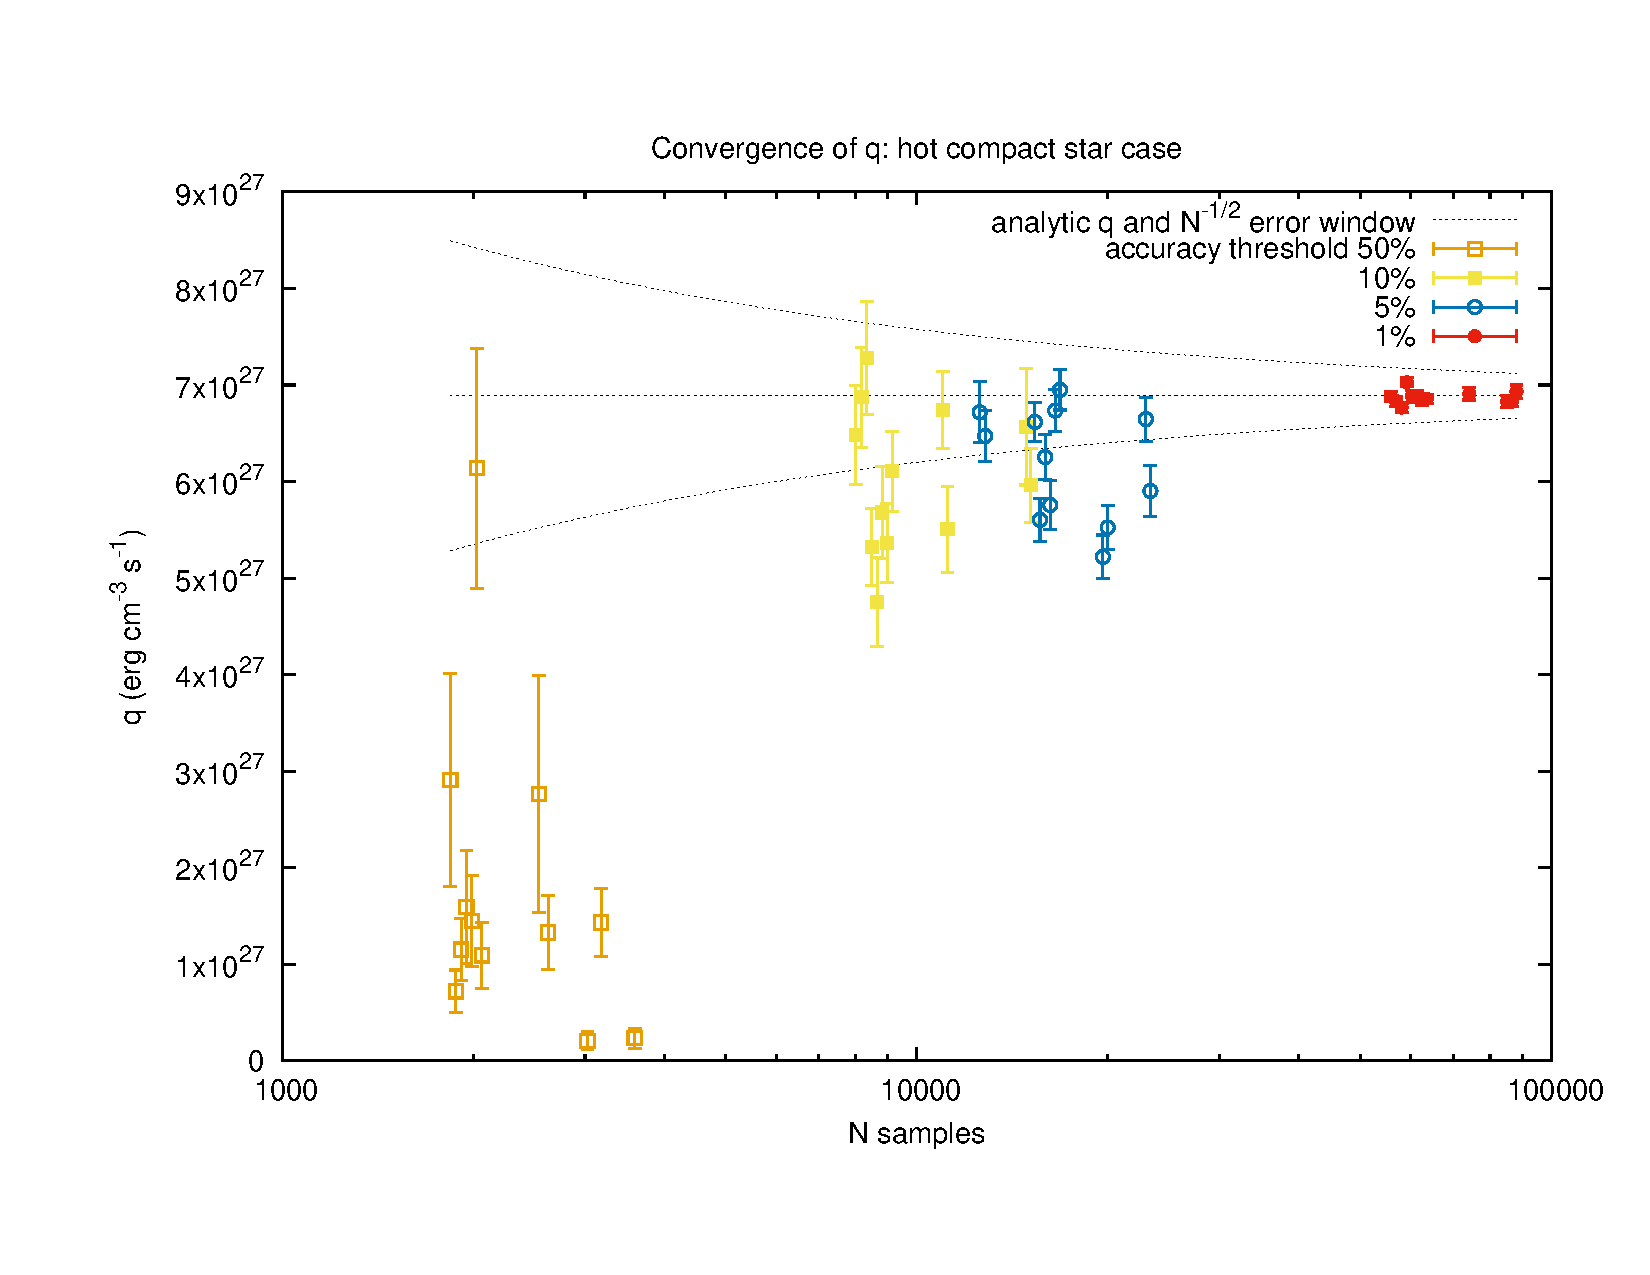
\includegraphics[width=16cm]{Figures/convergence_asano_fukuyama}
  \caption[Convergence of $q_{\nu\bar{\nu}}$ in the hot compact star case]{
    Convergence of the integration estimating $q_{\nu\bar{\nu}}$ in the
    hot compact star case.
    See caption for Fig.~\ref{fig:convergence_homo_mink} for description.
    (Note, the relative vertical range in this figure is signicantly larger
    than the range in Fig.~\ref{fig:convergence_homo_mink}.)
  }
  \label{fig:convergence_af_sphere}
\end{figure}

Fig.~\ref{fig:convergence_af_sphere} shows the results of a suite of
computations at increasing accuracy thresholds.
Unlike the homogeneous Minkowski case, here the Vegas algorithm
systematically underestimates $q_{\nu\bar{\nu}}$ at low resolutions.
For an accuracy of 10\% in this more realistic case, we need to compute
$\sym3\times10^4$ samples of the integrand.
\todo{catalog other sources for error in this case}

\section{$q_{\nu \bar{\nu}}$ for this Accretion Disk}
\label{sec:q_this_case}
We calculate $q_{\nu\bar{\nu}}$ above the accretion disk, on a unigrid, to make
an estimate of $Q_{\nu\bar{\nu}}$ (Eqn.~\ref{eqn:Q_vol}):
the power at infinite separation from the source, available to drive a jet.
In cartesian coordinates, the volume integration is decomposed
$\diff^3 x=\sqrt{-g}\, \diff x\,\diff y\,\diff z$.
\todo{add redshift factor for time}
Because of the approximate axial- and reflection-symmetry of the disk, we only
calculate $q_{\nu\bar{\nu}}$ over one octant and multiply $Q_{\nu\bar{\nu}}$ by
eight.
\todo{explain treatment of on-axis points}
The octant is shown in a meridional slice in Fig.~\ref{fig:q_grid}.
Because of the steep dependence of the annihilation rate on the relative angles
between incoming neutrino trajectories, $q_{\nu\bar{\nu}}$ falls off steeply
with distance from the bright inner region of the funnel: the rate decreases with
$r^{-8}$ at large enough distances that the source is approximately spherical
\citep{seti2006-nunubar}.
\todo{fix cite}
Thus, the annihilation rate at points outside the integration grid is negligible.
In fact, the computed local annihilation rate, shown in
Fig.~\ref{fig:q_rate_meridional},
confirms that $q_{\nu\bar{\nu}}$ falls off by many orders of magnitude at the
edges of this grid.
\todo{how large $N$?}

\begin{figure}
  \centering
  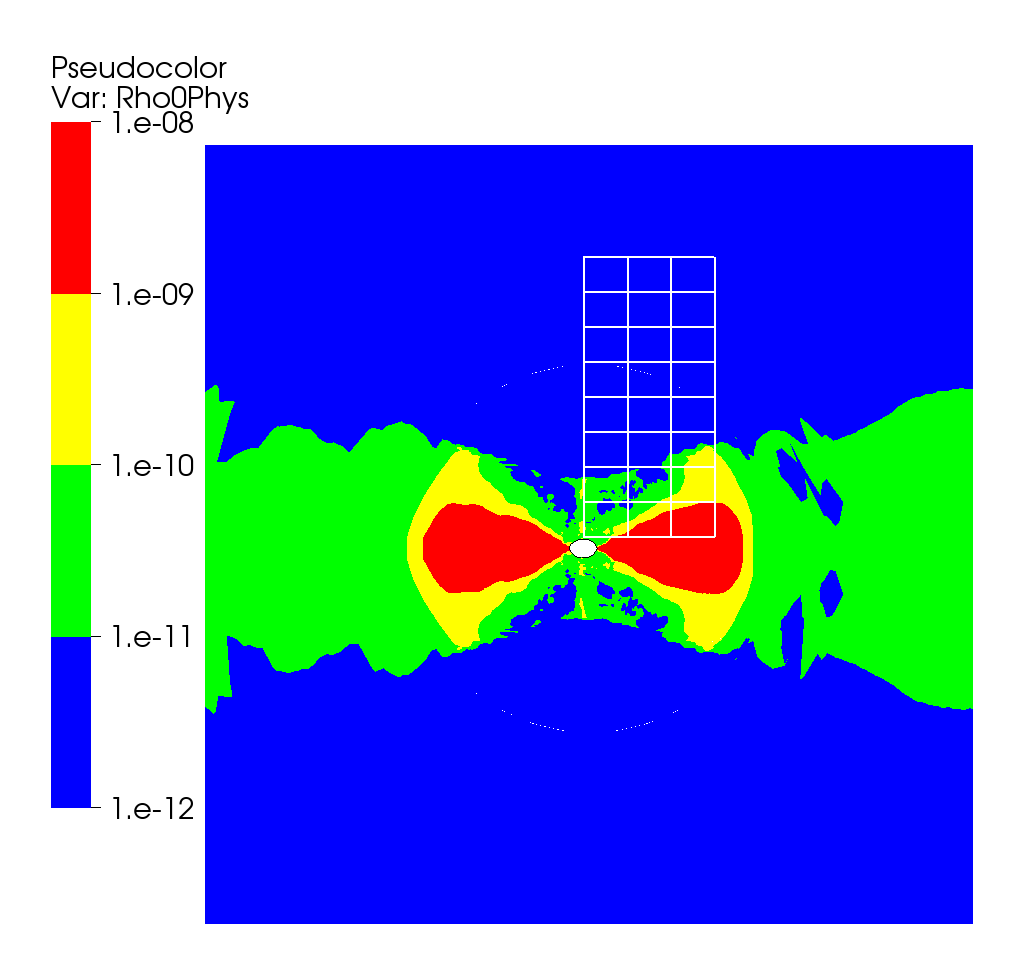
\includegraphics[width=10cm]{Figures/annihilation-slice}
  \caption[Grid used for the volume integral of $q_{\nu\bar{\nu}}$]{
    Meridional slice of the grid used to compute the spatial volume
    integral $Q_{\nu\bar{\nu}}=\int\diff^3 x\,q_{\nu\bar{\nu}}$ over one octant
    of the disk. The grid is composed of $4\times4\times9=144$~points,
    and extends 90~km, 90~km, and 192~km in the x-, y-, and z-directions,
    respectively.
    Decades of fluid rest density are plotted in units of
    $M_\odot^{-2}\sim10^{18}$~g~cm$^{-3}$.
  }
  \label{fig:q_grid}
\end{figure}

\begin{figure}
  \centering
  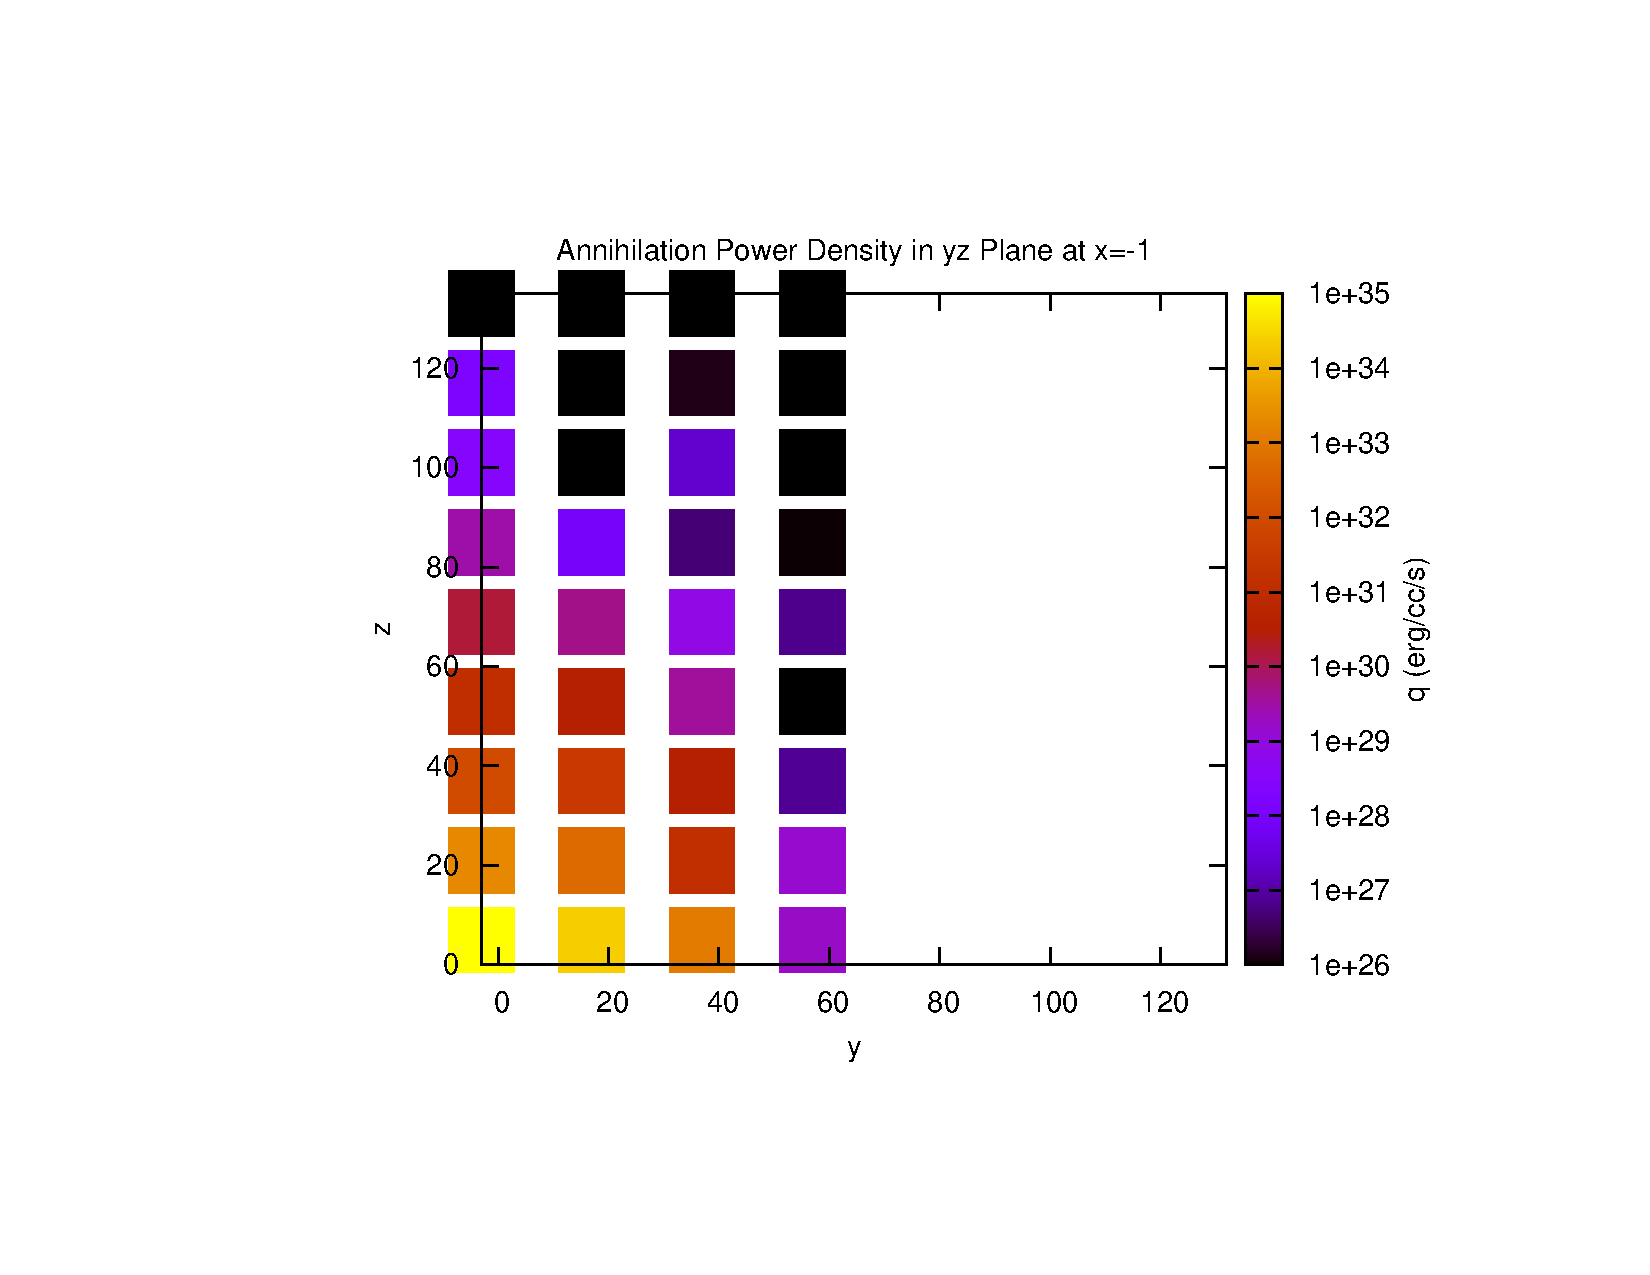
\includegraphics[width=13cm]{Figures/annihilation_rate_x-1}
  \caption[$q_{\nu\bar{\nu}}$ at the grid points]{
    Meridional slice of the annihilation rate in the y-z plane of the grid
    depicted in Fig.~\ref{fig:q_grid}. The axes are labeled in units of
    $M_\odot\sim1.5$~km.
  }
  \label{fig:q_rate_meridional}
\end{figure}

\subsection{Excluding Some Points from the Integral}
\label{ssec:excluding_pts}

The goal of our calculation is to estimate the free energy available to drive
a jet---energy carried by a superheated electron-positron pair plasma expanding
primarily away from the disk. But the simple volume integral of the points in
Fig.~\ref{fig:q_rate_meridional} includes the thermal energy of some plasma
that is headed for the black hole, and some plasma that that will be re-absorbed
by the nuclear fluid via the $\beta$-capture reactions,
$e^{-}\,p \rightarrow \nu_e\,n$ and
$e^{+}\,n \rightarrow \bar{\nu}_e\,p$.
We account for both of these losses in an approximate way by discarding points
from the volume integral at which these processes happen faster than the
explosion.

We can compare the timescales of these processes to the explosion timescale,
%which is a local estimate for how rapidly the plasma evacuates its place of
%origin, $x^j$:
%\begin{equation}
%  T_{\rm exp}(x^j) \sim \frac{q_{\nu\bar{\nu}}}{\rho}
%\end{equation}
%where $\rho$ is the rest density, which we can estimate from
%Fig.~\ref{fig:q_grid} as $\sym10^{-11}\,M_\odot^{-2}$ in the funnel region.
%\todo{untrustworthy; that's atmosphere}
which is a global estimate for how rapidly the plasma evacuates the funnel:
\begin{equation}
  T_{\rm exp} \sim \frac{L}{c_s}
\end{equation}
where $L\sim100\,M_\odot\sim0.5$~ms is the characteristic size of the funnel, and
$c_s\sim1$ is the sound speed, which is very high at these densities and
temperatures;
\todo{check $c_s$}
thus we estimate $T_{\rm exp} \sim 1$~ms.
Energy transfer processes occuring on a timescale shorter than this will quench
the explosion. We examine the processes of accretion and $\beta$-capture below.

\subsubsection{Accretion}
\label{sssc:accretion_timescale}
Very near the black hole, accretion dominates the energy transfer processes:
radiative and kinematic processes can't compete.
Energy deposited by neutrino-antineutrino annihilation in these regions
disappears into the black hole. Fig.~\ref{fig:timescales} shows the
advection timescale:
\begin{equation}
  T_{\rm adv} \sim \frac{r}{v^r}
\end{equation}
where $r$ is the radial distance from the black hole, and $v^r$ the radial
component of the fluid velocity.
Only within $r<30$~km does this process compete with the explosion.
However, this is a very rough estimate. The noise visible in the funnel region
of Fig.~\ref{fig:timescales} is due to the low densities there, where we cannot
accurately evolve the hydrodynamics equations, and where at some points,
we impose a slow-moving, low-density atmosphere, as described in
Sec.~\ref{sec:Methods}.

\begin{figure}
  \centering
  \begin{subfigure}{.45\textwidth}
    \centering
    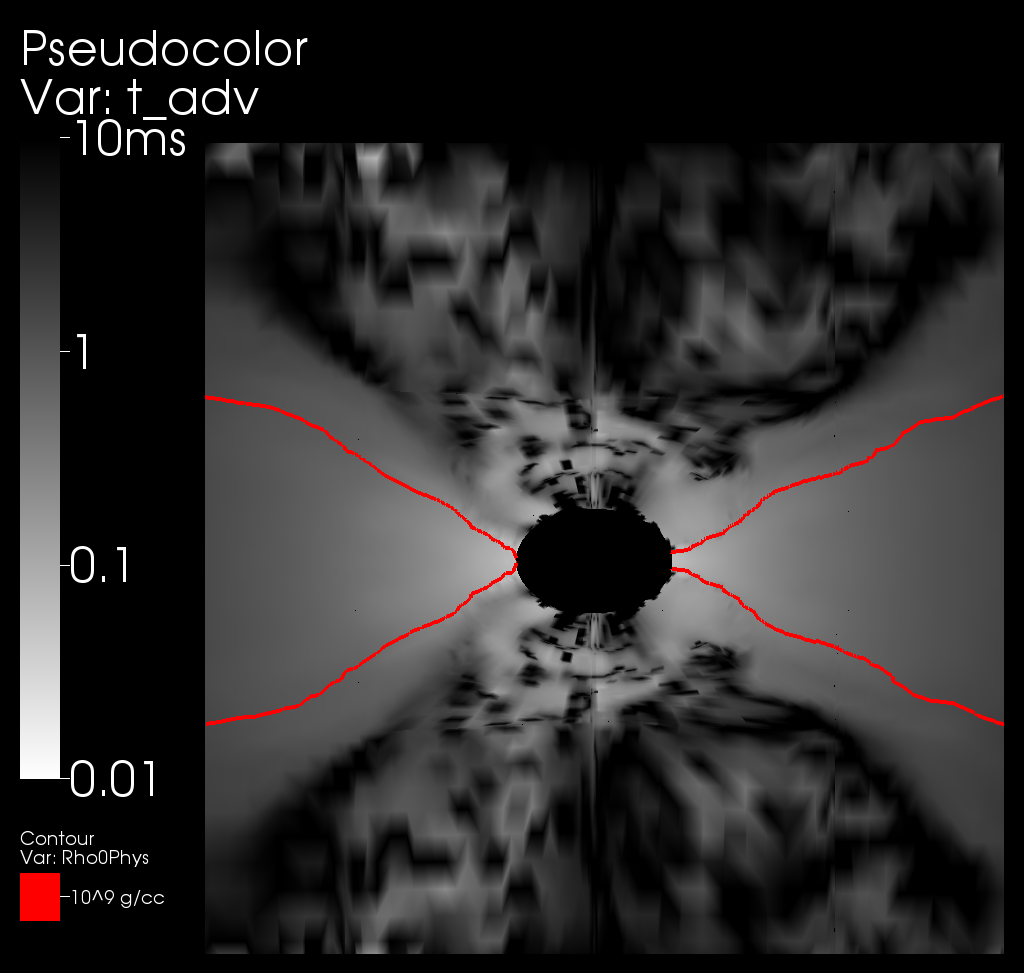
\includegraphics[width=1\linewidth]{Figures/timescales-slice-tadv}
  \end{subfigure}
  \begin{subfigure}{.45\textwidth}
    \centering
    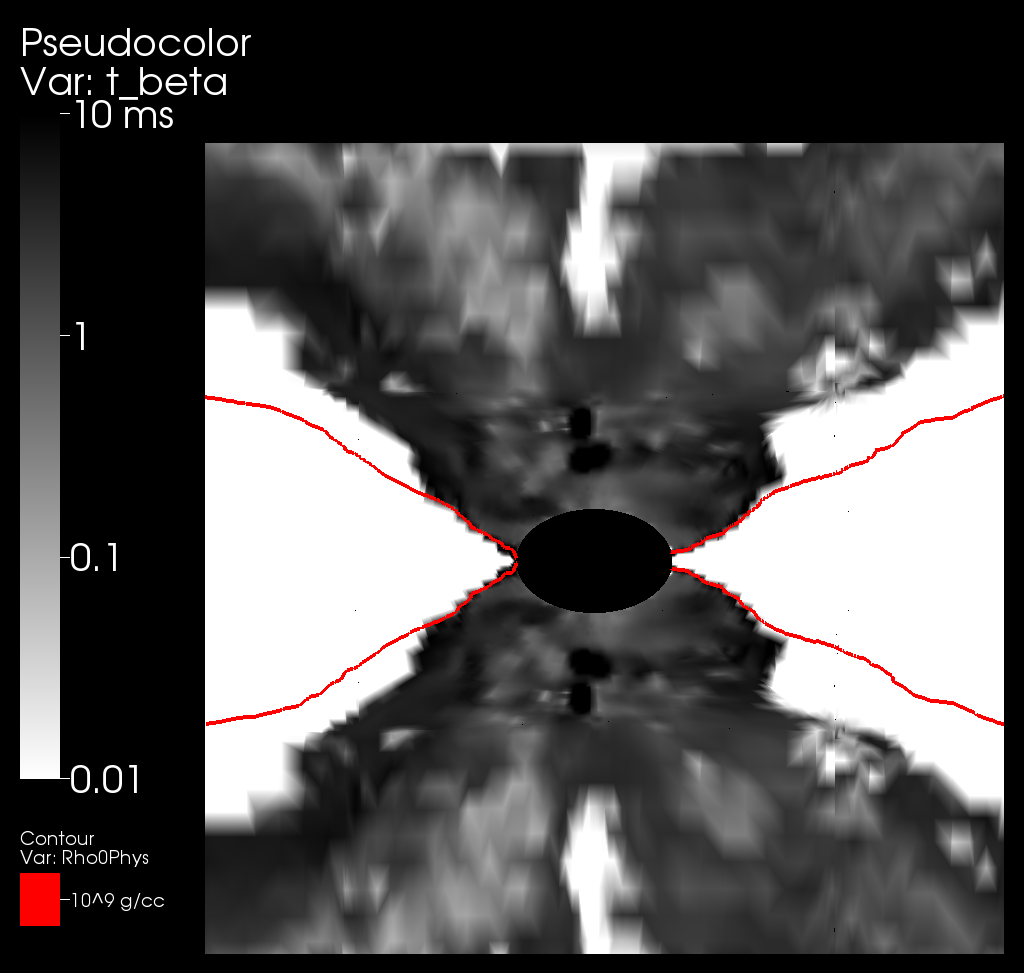
\includegraphics[width=1\linewidth]{Figures/timescales-slice-tbeta}
  \end{subfigure}
  \caption[Colormaps of explosion-quenching timescales]{
    Meridional slices of the timescales of two explosion-quenching processes,
    zoomed-in on the region $r\lesssim40$~km.
    The red density contour is drawn at $10^9\,{\rm g\,cm^{-3}}$.
    The oval in the center is the black hole horizon.
    Where $T\lesssim1$~ms, that process quenches the explosion.
    \emph{Left panel}: $T_{\rm adv}$ is noisy, and we can't really trust it in the
    funnel region, where we impose a false atmosphere at some points (described in
    Sec.~\ref{sec:Methods}).
    But I estimate that it is less than 1~ms within
    approximately three horizon-radii of the center.
    \emph{Right panel}: $T_\beta$ is clearly less than 1~ms only within the
    bulk of the disk.
  }
  \label{fig:timescales}
\end{figure}

\subsubsection{$\beta$-Capture}
\label{sssc:accretion_beta}
Deep inside the disk, the electron-positron pair plasma created by the
neutrino-antineutrino annihilation gets recaptured by nucleons, transferring
energy away from the plasma.

Fig.~\ref{fig:timescales} shows the $\beta$-capture timescale:
\begin{equation}
  T_\beta \sim \frac{n_b}{R_{\nu_e}+R_{\bar{\nu}_e}}
\end{equation}
where $n_b$ is the baryon number density, and $R_{\nu_e}$ and $R_{\bar{\nu}_e}$
are the local leakage lepton-number emission rates, a rough estimate for the
\todo{how good?}
rates of the $\beta$-capture reactions (see Sec.~\ref{sec:leakage}).
This timescale is much larger than 1~ms inside the funnel, where it may be
neglected, and much less than 1~ms inside the disk, where it quenches the
explosion.

\subsection{Back-of-the-Envelope Estimate of $Q_{\nu\bar{\nu}}$}
\label{ssec:back_of_envelope_Q}
Excluding points affected by these explosion-quenching processes, we can make an
estimate of the power at infinite separation:
\begin{equation}
  Q_{\nu\bar{\nu}} \approx 4 \pm 0.5 \times 10^{52}\, {\rm erg\,s^{-1}}\nonumber,
\end{equation}
where I have summed $q_{\nu\bar{\nu}}$ using a simple midpoint-rule
\todo{include $\pm$ order-of-mag for numer res}
\todo{add/explain redshift term}
numerical integration,
\todo{estimate midpoint err, goes as $q_{\nu\bar{\nu}}''$}
and the uncertainty is the volume integral of the uncertainties estimated by the
Monte Carlo algorithm, which we guess to be an underestimate, from the results
of the hot, compact star test in Sec.~\ref{sssc:q_af_sphere}.

To order-of-magnitude, this power is maintained for the lifetime of the disk,
$T_{\rm dep}\sim200$~ms (see Sec.~\ref{sec:scales}). Thus
\begin{equation}
  E_{\rm jet} \approx 10^{52} \, {\rm erg} \nonumber,
\end{equation}
which is comparable to the brightest luminosities and durations observed for
shoft duration gamma ray bursts:
\todo{cite Nakar 2007}
\begin{eqnarray}
  L &\sim& 10^{50\text{--}52} \, {\rm erg s^{-1}} \nonumber\\
  \langle T_{90} \rangle &\sim& 100 \,{\rm ms}. \nonumber
\end{eqnarray}
\todo{actually, $E_{\rm jet}$ is larger by factor of 10}
We conclude that in this case of a high-spin black hole and massive accretion
disk, neutrino-antineutrino annihilation is a viable candidate alone to power a
gamma ray burst.

The two serious limitations of this back-of-the-envelope calculation,
however, is 1) the error in the numerical integration over the spatial volume,
which we could improve with a Monte Carlo integration over that volume,
and 2) the numerical noise and lack of information about the state of the matter
in the funnel.
\todo{also related to lack of info about baryon loading}



% Conclusion
\chapter{Conclusion}
\label{chap:conc}

\section{What are the Major Effects of Neutrinos in this Case?}

\section{How Relevant is this to All Classes of Mergers?}

\section{What Remains to be Done?}

\newpage

% Appendix
%\begin{appendix}
%  \chapter{Things You Should Already Know}
%  \input{50-appendix}
%\end{appendix}

\bibliography{references}

\end{document}
